\documentclass[english, LaM, oneside]{sapthesis}%remove "english" for a thesis written in Italian
%Bachelor's (laurea triennale) thesis : Lau 
%Master's (laurea specialistica) thesis: LaM 
%PhD's thesis: PhD 
\usepackage[utf8]{inputenx}
\usepackage{indentfirst}
\usepackage{microtype}
\usepackage{pdfpages}
\usepackage{graphicx}
\usepackage{lettrine}
\linespread{2}
\usepackage[nottoc, notlof, notlot]{tocbibind}
\usepackage{hyperref}
\usepackage{booktabs}
\usepackage{adjustbox}
\usepackage{float}
\usepackage{xurl}
\hbadness=99999

\hypersetup{
			colorlinks=true,
			linkcolor=red,
                        linktoc=page,
			anchorcolor=black,
			citecolor=red,
			urlcolor=blue,
			pdftitle={Design and reference implementation of a standard for rent and layaway of non-fungible tokens in EVM-compatible blockchains},
			pdfauthor={Palermo Andrea},
			pdfkeywords={thesis, sapienza, roma, university}
 }

\title{Design and reference implementation of a standard for rent and layaway of non-fungible tokens in EVM-compatible blockchains}
\author{Andrea Palermo}
\IDnumber{1810218}
\course[]{Computer Science}
\courseorganizer{Facolt\`a di Ingegneria dell'informazione, informatica e statistica}
\submitdate{2021/2022}
\copyyear{2023}
\advisor{Prof. Claudio Di Ciccio}
\authoremail{palermo.1810218@studenti.uniroma1.it}
%\examdate{X March 2023}
%\examiner{Prof. ...} \examiner{Prof. ...} \examiner{Prof. ...}  \examiner{Prof. ...}  \examiner{Prof. ...} \examiner{Prof. ...}  \examiner{Prof. ...} 

%we refer to http://ctan.mirrorcatalogs.com/macros/latex/contrib/sapthesis/sapthesis-doc.pdf for an exhaustive description of the sapthesis documentclass.


\begin{document}

\frontmatter
\maketitle
\begin{abstract}
\label{chap:abs}
Non-Fungible Tokens (NFTs)\cite{ref:nfts} are digital assets that represent ownership or proof of authenticity of a unique item or piece of content, such as a piece of art, music, or a real world good. Unlike fungible tokens (cryptocurrencies), each NFT is unique and cannot be split in sub-units or exchanged on a one-to-one basis with another token. NFTs use blockchain technology to verify ownership and authenticity, making them highly secure and resistant to counterfeiting. The popularity of NFTs has grown in recent years, leading to the creation of NFT marketplaces and the rise of NFT-based collectibles, digital art, and other types of assets (in the form of both physical and digital objects). However, one of the main challenges faced by NFT owners is the lack of liquidity. While NFTs are valuable, they cannot be easily converted into money, which limits their use and potential value.\newline 
This limitation, together with the fact that assets represented as NFTs are intrinsically well suited to be rented and layawayed, led rental and layaway services to become very important sectors within the Non-Fungible Token ecosystem. These concepts allow for NFT owners to layaway or rent out their assets to others, offering a new level of liquidity and monetization capabilities for NFT holders and creating new opportunities for NFT enthusiasts to gain access to unique and valuable NFTs without having to purchase them outright.\newline 
The aim of this work will therefore be the analysis of the existing approaches to NFT rental and layaway, the identification of their limitations and the proposal of a novel solution which tries to mitigate them.
\end{abstract}

\tableofcontents

\mainmatter
\chapter{Introduction}
\lettrine[lines=2, findent=3pt, nindent=0pt]{N}{}on-fungible tokens represent ownership of unique physical or digital assets, such as artworks or music, or even a real apartment. They are stored on a blockchain, which provides a secure and transparent record of ownership, and their usage has enabled the creation of new marketplaces and revenue streams. As the popularity of NFTs has grown, so too has the interest in alternative ways to acquire them. Two such methods are NFT rental and NFT layaway.
NFT rental is a concept similar to traditional rental arrangements, such as renting a car or a vacation home. With NFT rental, users can enjoy the benefits of owning an NFT for a limited time, without needing to make a large upfront payment or take on the long-term responsibilities of ownership.
This concept allows for NFT owners to rent out their assets for a specified period of time, during which the renter can use the NFT for their own purposes. This can include displaying the NFT in a virtual gallery, using it in a video game or gaining access to the usage of a physical asset. The renter pays a fee for the privilege of using the NFT, and the owner earns passive income from the rental.\newline
NFT layaway, on the other hand, is a payment plan that allows individuals to acquire a NFT over time. Similarly to traditional layaway plans, individuals make a series of smaller payments over a set period, after which they keep ownership of the NFT. This allows individuals to spread the cost of acquiring an NFT over a longer period, making it more accessible to those who may not have the funds to purchase it outright. In fact, it is very similar to a bank loan, with which customers can buy a good and pay for it over a certain amount time, but without needing a centralized intermediary (the bank) who loans money to the buyer. This is possible because when the layawayed asset is an NFT, the layaway can be managed by a decentralized intermediary, namely a smart contract, which has the capability of foreclosing the token from the layaway receiver if they fail to pay for it on time: this will ensure that the person who sold the token will either get all installments payments or the token back, therefore eliminating the need of a third entity which loans money to the buyer.\newline
Currently, the state-of-the-art token standard mainly used for building NFT collections on Ethereum blockchain is the ERC-721 standard\cite{ref:EIP721} (an interface which defines the basic functionalities of a NFT). This works focuses on Ethereum as it is the blockchain on which most of the existing NFTs are built. Ethereum standards and smart contracts are written in Solidity, the most common Ethereum programming language. Moreover, there exist a lot of other blockchains which can run the same smart contracts that run on Ethereum: this is possible thanks to the Ethereum Virtual Machine\cite{ref:EVM}, which allows Solidity smart contracts bytecode to be executed on any type of machine (similarly to what JVM does for JAVA). This led many other blockchains to make use of the EVM: these chains are referred to as \textit{EVM-compatible chains}; some of the most known ones are Polygon, Optimism, Arbitrum, Binance Smart Chain and Avalanche. Therefore, almost every NFT currently existing on EVM-compatible chains implements the ERC721 standard.
Whereas this standard has no problems in dealing with all basic NFT operations, it doesn't define primitives to allow the temporary usage grant of tokens (namely, rental and layaway).\newline
Thus, the aim of this work consists in designing and developing a NFT standard which extends ERC721 adding token rental and layaway capabilities. Being ERC721 standard common to all EVM-compatible blockchains, also the new proposed standard will be usable on any of these chains.\newline
For the sake of readability, this document will focus on a concrete application scenario which is currently gaining much traction, namely the fractionalization of apartments in the form of NFTs. These tokens can represent portions of an apartment and be managed each by their potentially different owner, and represent a perfect example of how rental and layaway capabilities can improve the usage of NFTs. All the features and benefits of NFT real estate and apartment fractionalization, together with other interesting potential NFTs applications, are scrupulously analyzed in \cite{ref:NFT applications}.
From now on, we will assume for simplicity that each room of the apartment is bound to a different NFT; the access to a particular room will be granted only to the owner of the token bound to the room. This can be enforced by a simple system installed on doors that retrieves the owner of the room token on-chain and then verifies that the signature of the person trying to access matches the retrieved owner; if the verification succeeds, the door will then unlock itself. Using this approach, room token owners can access in a simple and direct way to the corresponding rooms, even during a rental or a layaway.

\section{Advantages over collateral lending}
Even if there exist a lot of NFT lending services out there, the concept of on-chain lending requires the borrower to deposit a collateral, whose value is often greater than the borrowed token value, in order to be able to reimburse the lender if the borrower doesn't return the token. This is a major limitation: NFT users are not able to gain usage rights of the token without having to deposit its entire value immediately. Moreover, the borrower has to constantly monitor the value of its collateral: if it becomes less than the borrowed value, the borrower gets liquidated, incurring in a so called liquidation fee; the liquidation consists in the borrowed token being returned to the lender, and the collateral (minus the liquidation fee) being returned to the borrower. The liquidation fee is needed to pay for bots who monitor and execute liquidations and sometimes also to sustain the lending protocol. A more in depth analysis of liquidations mechanisms can be found in \cite{ref:liquidation}.\newline
These limitations make rental and layaway much preferrable to lending with collateral, as they can grant NFT usage rights without an entire upfront payment and do not suffer liquidations risks. 

\bigskip
\bigskip
\bigskip
\bigskip
In \hyperref[chap:1]{Chapter~\ref*{chap:1}} we briefly describe the current state of the art in the fields of NFT layaway and rental and its limitations.

\bigskip
In \hyperref[chap:2]{Chapter~\ref*{chap:2}} we show our proposed solution, summarizing its advantages over the state of the art and describing its structure and architecture in depth.

\bigskip
In \hyperref[chap:3]{Chapter~\ref*{chap:3}} we evaluate the proposed solution's reference implementation, also showcasing the performed unit tests.

\chapter{State of the art}
\label{chap:1}
In this chapter we will showcase some of the existing implementations of rental and layaway services in the Ethereum and EVM-compatible chains ecosystem. Most of these solutions do not use a common standard, although there exists a standard approved by the Ethereum community for NFT rental, which we will discuss. For NFT layayway, on the other hand, there is no such standard, as far as the author knows.\newline
Concluding the chapter, we will also examine the potential limitations of the mentioned existing approaches.

\section{Rental}
For what concerns rental, as mentioned above, the Ethereum community has approved a token standard, named ERC4907\cite{ref:EIP4907}. This standard, as all Ethereum protocol changes or improvements, was approved in the form of an Ethereum Improvement Proposal (EIP). EIPs are submitted to the community by their authors, and get reviewed and possibly approved by an elected team of \textit{Ethereum editors}.\newline
This standard extends the ERC721 standard, the approved standard for non-fungible tokens on Ethereum ecosystem; however, ERC721 tokens lack of both rental and layaway capabilities, as they were not intended to be used as such.
As we said, ERC4907 standard extends ERC721, with the aim of making these tokens also rentable.\newline
In order to understand how the EIP4907 authors meant to do so, we must first dive a little in the features of ERC721 NFTs. First of all, a ERC721 token has an owner, who is able to transfer the token to other accounts; the owner can also give their approval to a specific account in order to also allow it to transfer the token. ERC721 tokens are organized in so called collections: a single ERC721 contract can emit (\textit{"mint"}) various tokens, which will be part of a collection. Implementing rental services only using ERC721 capabilities is not possible, mainly because when an account owns a token they can always transfer it or change the address approved for transfers as they will, and this is not suitable for rental: there is no way to make sure that an account who temporarily owns a rented token will transfer it back at the end of the rental period. Even if an intermediary smart contract manages the rental making sure that the rental receiver approves the rented token's transfer rights to its contract's address, there is no guarantee that the receiver will not change their approval or transfer the token in a second moment during the rental period, causing the contract not to be able to transfer the token anymore.\newline
Of course, any smart contract programmer could come up with their own implementation of rentable NFTs which extends ERC721 standard overcoming these issues, but these solutions would not conform to a common standard, which would make the usage of these tokens much more complex and disorganized.\newline
EIP4907 is in fact a tentative of creating such a standard: the authors manage to do so by adding an additional role other than the token owner, called \textit{user}. The user represents the receiver of a rental, and when the rental period ends, the user gets deleted. However, this solution has some important limitations, which will be discussed at the end of the chapter.\newline
Other tentatives have been made within EVM-compatible chains in order to implement ERC721 NFTs rental without creating a new token standard. These approaches overcome the issue of the missing capabilities of ERC721 tokens mentioned above by creating a so called \textit{wrapped} version of the tokens using an escrow contract: when some account A wants to rent a token to another account B, the escrow contract holds the real ERC721 token for the whole rental period, giving to account B a wrapped version of the token; owning this wrapped token implies being the receiver of the rental, hence it should allow usage the token. However, this last implication is not directly guaranteed by the smart contracts, as the tokens are often used off-chain: this is the major limitation of these type of solutions, which again will be discussed at the end of the chapter.
Two of the most known examples of this approach are ReNFT\cite{ref:renft} and Vera Finance\cite{ref:vera}, which offer rental and \textit{rent-to-buy} services on different EVM-compatible blockchains.


\section{Layaway}
NFT layaway, on the other hand, is a sector that has not currently been investigated as much as rental, and in fact lacks a standard approved in the form of an EIP. As far as the author knows, there is no proposed EIP of this kind that has not been approved yet.\newline
Also for layaway, a similar issue to the one discussed above regarding rental still holds: if a token is transfered to the layaway receiver, there is no guarantee that they will pay all the agreed installments on time, and if they do not there is no way of foreclosing the token from them to return it to the original owner just using ERC721 functionalities.\newline
However, there are some solutions which overcome this difficulties, again using a method similar to the one seen for the rental, namely holding NFTs in an escrow account.\newline 
One example of this approach is represented by Supermojo\cite{ref:supermojo}, which implements a very simple simple model: the token under layaway is put in an escrow contract until all installment have been paid; after payments are completed, layaway receiver will be able to take the token out of the escrow account.\newline
Another somehow different example is Teller Finance\cite{ref:teller}, which proposes a  particular layaway model. This is how their scheme works: after putting down a down payment of up to 50 percent of the token value, users who want to receive the layaway would be matched with a lender who can meet the other half.
The NFT would then be placed in the escrow account until the layaway receiver makes all their installment payments on time. Only when these payments have been completed, the user can receive the true ERC721 token.\newline
Again, the limitations of these types of approaches will be examined in the last section of the chapter.

\section{State of the art solutions' limitations}
In this section we will showcase the limitations of the solutions described above.\newline
For what concerns rental, we first examine ReNFT and Vera Financial's approach (which from now on we will denote as \textit{escrow-wrap} model). The greatest limitation of this type of solution, as hinted above, is the fact that owning the wrapped version of a NFT does not automatically guarantee its usage rights. To be more specific, concrete usage of assets bound to NFTs happens off-chain: in our apartment fractionalization setting, for instance, the rooms are obviously physical assets whose usage right is granted by granting access to them; access has to be granted by an off-chain system like the one we described, simply because a smart contract will never be able to directly act on physical or off-chain objects. This entails that the off chain usage rights granting system of assets bound to NFTs can be programmed arbitrarily by its developer: this is the reason why we can state that being the owner of a token does not \textit{automatically} grant its usage rights. Of course, what usually happens is that the off-chain platforms where the NFT assets can be used will grant usage rights to the owner of the token (as it is the role defined in ERC721 standard as the proprietor of the token). However, as we explained, this is not automatic and cannot be enforced on-chain.
Another example can be done for NFTs representing in-game assets: the videogame will allow usage of a token only to its owner.\newline
As we can easily imagine, this is an important limitation for the \textit{escrow-wrap} model, as the wrapped tokens are managed by a separate contract (different from the contract who manages the original token), so it is not likely that off-chain usage rights granting systems will take into account this different contract address in order to fetch the owner of the NFT. A possible solution would be modifying these systems in order to also check the new wrapper contracts' addresses, but it would not be very suitable and straightforward, as it would have to be done for each token collection and wrapper contract separately: if an off-chain system is in charge to grant usage rights of many different ERC721 token collections, it would have to try to fetch the owner of a token from its collection's contract and each possible wrapper contract. Moreover, the list of all these wrapper contracts would not be well-defined, as any developer can come up with its own new wrapper contract at any moment. Additionally, as stated before, these type of contracts do not necessarily extend a common standard, which makes their usage quite inconvenient, as there is no standard way to use their functionalities. \newline
Other than this, there exist also other less impactful limitations of the \textit{escrow-wrap} model: the wrapper and escrow contracts constitute an additional potential point of failure other than the ERC721 contract which mints tokens; this implies that these additional contracts must gain the trust of NFT users.\newline
Moving on to the other discussed rental approach, namely EIP4907, we can examine its own limitations compared to the previously discussed ones. First of all, ERC4907 suffers a limitation similar to the one discussed for the \textit{escrow-wrap} model. In particular, the addition of the user role causes some ambiguity and retro-compatibility issues: as seen before, when there exist more roles other than the token owner, the off-chain platform where the NFT assets are used can arbitrarily assign usage rights to any of them. Having the additional user role, the choice of whom should be granted usage rights is left to the off-chain platform. This can create ambiguities and also retro-compatibility issues, as before the creation of ERC4907 standard only the owner role existed, hence many of the existing platforms will grant usage rights to the owner, having no notion of the user.\newline
Additionally, the reference implementation provided with EIP4907 suffers some problematic implications: as it is written, it seems to let the owner of a rented token change the rental user and deadline at any time, and also transfer the token during the rental period, deleting the user (therefore stopping the rental). This is not suited if we want the rental service to be trustless, in the sense that rental provider and receiver can use the service without having to trust each other. Using ERC4907 reference implementation, the receiver has to trust the provider, as they will be able to end the rental whenever they like. This is not quite appropriate, as blockchains and tokens living on them are mostly meant to be used in a trustless way (without having to trust a centralized entity).
The EIP authors have also built a working ERC4907 renting application, named Double Protocol\cite{ref:double}, but it is not clear from the project's documentation how they tried to overcome this limitation. \newline
For what concerns layaway, on the other hand, we have seen that the most known existing solutions again use a \textit{escrow-wrap} model. Hence, the limitations of these approaches are analogue to the ones described for \textit{escrow-wrap} rental: again, the platform which grants tokens' usage rights should check the tokens' ownership on all potential wrapper contracts, not necessarily in a standard way.


\chapter{Proposed solution}
\label{chap:2}
In this chapter we will showcase our proposed solution, describing all of its features and how it can improve the current NFT rental and layaway state of the art. \newline
The main idea upon which this solution is based consists in avoiding the creation of new roles (as seen for the user role in ERC4907 standard) and also shifting from the \textit{escrow-wrap} model, as we have discussed the limitations that these approaches imply. \newline
In particular, rental and layaway receivers will be set as owners of the rented or layawayed tokens, as the owner role is the only role natively supported by ERC721 standard. At this point, it becomes more clear why we need to extend the ERC721 features by creating the ERCX standard: the added functionalities will allow rented tokens to be returned to the rental provider when rental expires, and layawayed tokens to be foreclosed and returned to layaway provider if the agreed installments are not paid. The new standard will also make sure that rental and layaway receivers will not be able to arbitrarily transfer the the received tokens token during rental or layaway period, which would make impossible to return the tokens to the providers. \newline
Rental and layaway methodologies will be discussed more in depth in the following sections.

\section{Rental}
An ERCX token rental can be started in two different modalities, depending on whether rental provider and receiver trust each other.\newline If they do trust each other, they can simply find an agreement on the rental price and duration; at this point the provider will start the rental, and the receiver will have to pay the agreed price. The receiver is not forced to make the payment, and this is why the provider must trust them: if the receiver doesn't pay the agreed price, they will still be the owner of the rented token for the whole agreed period, and there is nothing the provider can do to claim the token back. If, contrarily, the receiver pays the provider before they start the rental, the receiver is not guaranteed that the provider will actually start the rental. These implications will probably cause this type of approach to be very seldom used, as public blockchains and NFTs are mainly meant to be used in a trustless manner.\newline
The second modality would instead enable a completely trustless rental agreement, hence it will be probably the most used one. This other procedure involves a rental intermediary, which could potentially be any blockchain account: there exist two type of blockchain accounts, namely Externally Owned Accounts (EOAs, which are owned by people and have non-deterministic behaviour) and contract accounts (smart contracts, with deterministic behaviour). This intermediary is nominated by the rental provider before the rental starts. An EOA can be chosen if both the provider and the receiver trust its owner: in this case they will all agree on a rental price and duration, and the intermediary will be trusted to start the rental only after the receiver's payment of the agreed price to the provider. Again, this solution is not ideal as it is not a trustless procedure. If, on the other hand, a smart contract is chosen as intermediary, the same procedure can be completed without the users needing to trust anybody, as the above mentioned operations would be immutably coded in the contract. A reference implementation of such an intermediary contract is contained in the GitHub repository of the project. This implementation lets the token owner make a rental proposal, specifying a duration and a price; eventually, a user interested in renting the proposed token will be able to accept the proposal paying the specified price, allowing the contract to start the rental. After a rental is started, any account will be able to terminate it and return the rented token to the provider, as long as the rental period is expired. \newline
Once a token is rented, ERCX standard provides many additional functionalities for the rental provider and receiver. First, a rented token can be subrented, if the account that rented it in the first place decides to allow it; the procedure used for subrenting is analogous to the one described for normal rental. \newline
Moreover, agreed rental period can be later extended, again using an intermediary which can be a contract or an EOA. Still, the procedure used to find an agreement on the extension period and price is very similar to the one seen for rental and subrental agreements, and is supported by the provided intermediary contract reference implementation. \newline
Other than this, the rental receiver can transfer the rented token to another account, while the provider can transfer his "rental ownership", in both cases without interrupting the rental; transferring rental ownership means that the provider of the rental will change and the new provider will get the token back at the end of the rental (and also further rental extension payments, if any). Both these transfer operations can be allowed or forbidden by the account that rents the token in the first place; if token is also subrented, these transfers can happen only at the last subrental level (the most recent one). \newline
Finally, a rented token can also be redeemed by the receiver, if they want to convert their rental in a definitive purchase. The agreement between provider and receiver will be reached once again using an intermediary, with the modality discussed above. \newline
All the discussed features will be described more in depth in the following diagrams sections.

\section{Layaway}
For what concerns layaway, we will see that many of the core functionalities work similarly to the ones discussed for rental. \newline
The first main difference is the fact that layaway must be started using an intermediary. The use of an intermediary is mandatory because it will be the entity entitled to terminate the layaway in the correct way: if all installments have been paid, the layawayed token will be kept by the layaway receiver; otherwise it will be foreclosed and returned to the provider. This intermediary can once again be an EOA or a contract account, and a reference implementation of a layaway intermediary contract is provided in the GitHub repository of the project. This contract works similarly to the one described for rental, as it lets token owners propose layaways specifying the number of installments, their amount and their frequency; an interested user will then have to pay the first installment to start the layaway, and keep paying the next ones if they don't want their token to be foreclosed. The layaway can be then terminated in two ways: before all installments have been paid, any account can request the intermediary to end the layaway and return the token to the provider, if the receiver is late on some installment payment; if, on the other hand, the receiver has yet made all payments on time, any account can request the intermediary to terminate the layaway, letting the receiver keep the token. \newline
Once more, ERCX standard provides some additional functionalities other than the simple layaway: the layaway receiver can transfer their token to another account, while the provider can transfer his "layaway ownership", in both cases without interrupting the layaway; transferring layaway ownership means that the provider of the layaway will change and the new provider will receive all further installments payments, and also get the token back if the receiver stops paying. transferring the token means instead that the receiver of the layaway will be changed, and the new receiver will have to pay further installments in order to keep the token at the end of the layaway. As expected, the transfer agreement will be reached using an intermediary; the provided intermediary contract reference implementation offers this capability. \newline
Also for layaway, all these functionalities will be showcased more in depth in the diagrams sections.

\section{Advantages over state of the art}
Having discussed the limitations of the existing implementations, we will now investigate how our solution will try to mitigate and solve them. \newline
With respect to the \textit{escrow-wrap} model, we have yet discussed how its usage entails having to rework the applications where rented or layawayed NFTs are used; with ERCX standard, this additional effort is not needed as the receiver account is set as token owner, that is the role to which every existing NFT application assigns usage rights, being it the only role defined in ERC721 token standard. Hence, the ERCX approach solves retro-compatibility issues, and also avoids creating ambiguities on where to check token ownership (whether on the ERC721 contract or the wrapped token contract).\newline
Moving on to the advantages over ERC4907 approach, we can first of all underline that ERCX tokens don't define any new role other than the token owner, whereas ERC4907 tokens define the above mentioned user role. This new role again causes retro-compatibility and ambiguity issues; the retro-compatibility is not guaranteed because, as stated above, existing ERC721 off-chain applications assign usage rights to the token owner. The ambiguity is instead created by the fact that only ERC4907 NFTs would have their user role defined, while normal ERC721 tokens wouldn't: this causes the off-chain systems to not exactly know who it should assign usage rights to. Again, with ERCX standard introduction all these issues would be solved, as it only relies on the owner role.

\section{Structural and behavioral diagrams}
%\label{sec:moons}
We can now proceed to analyze the diagrams describing the proposed solution, in order to understand precisely how each of the mentioned functionalities works.

\subsection{Storyboards}
The first diagrams to be presented are the storyboards; even if these type of diagrams are not conform to any UML diagram specification, they can be useful to understand how users will interact with rental and layaway services and which advantages will be granted by the usage of ERCX standard. As usual, storyboards have been made for each possible user scenario. They show how each scenario would take place with and without the usage of ERCX standard, in order to better understand the solution's advantages. The comparison has been made with \textit{escrow-wrap} solutions, as they are currently the most used out there, without considering ERC4907 standard solutions, as they are not much used and suffer of the discussed important limitations.\newline
As anticipated, the storyboards will specifically focus on NFT apartments rental application. For simplicity, here we will consider each NFT representing an entire apartment (not a portion of it). Each particular storyboard will now be commented in its own subsection.

\subsubsection{Rental}
This first storyboard (Fig.~\ref{fig:Rental SB}) shows how users are able to rent NFTs using existing state of the art solutions or ERCX standard. As discussed in the state of the art limitations section, the main advantage of introducing ERCX standard lies in the fact that the existing \textit{escrow-wrap} solutions must be integrated with the off-chain application where the rented NFTs are used, in order to grant usage rights to wrapped tokens owners. This requires an effort and possibly an investment by the managers of the mentioned application.

\begin{figure}
    \centering
        \begin{adjustbox}{width=1\textwidth}
            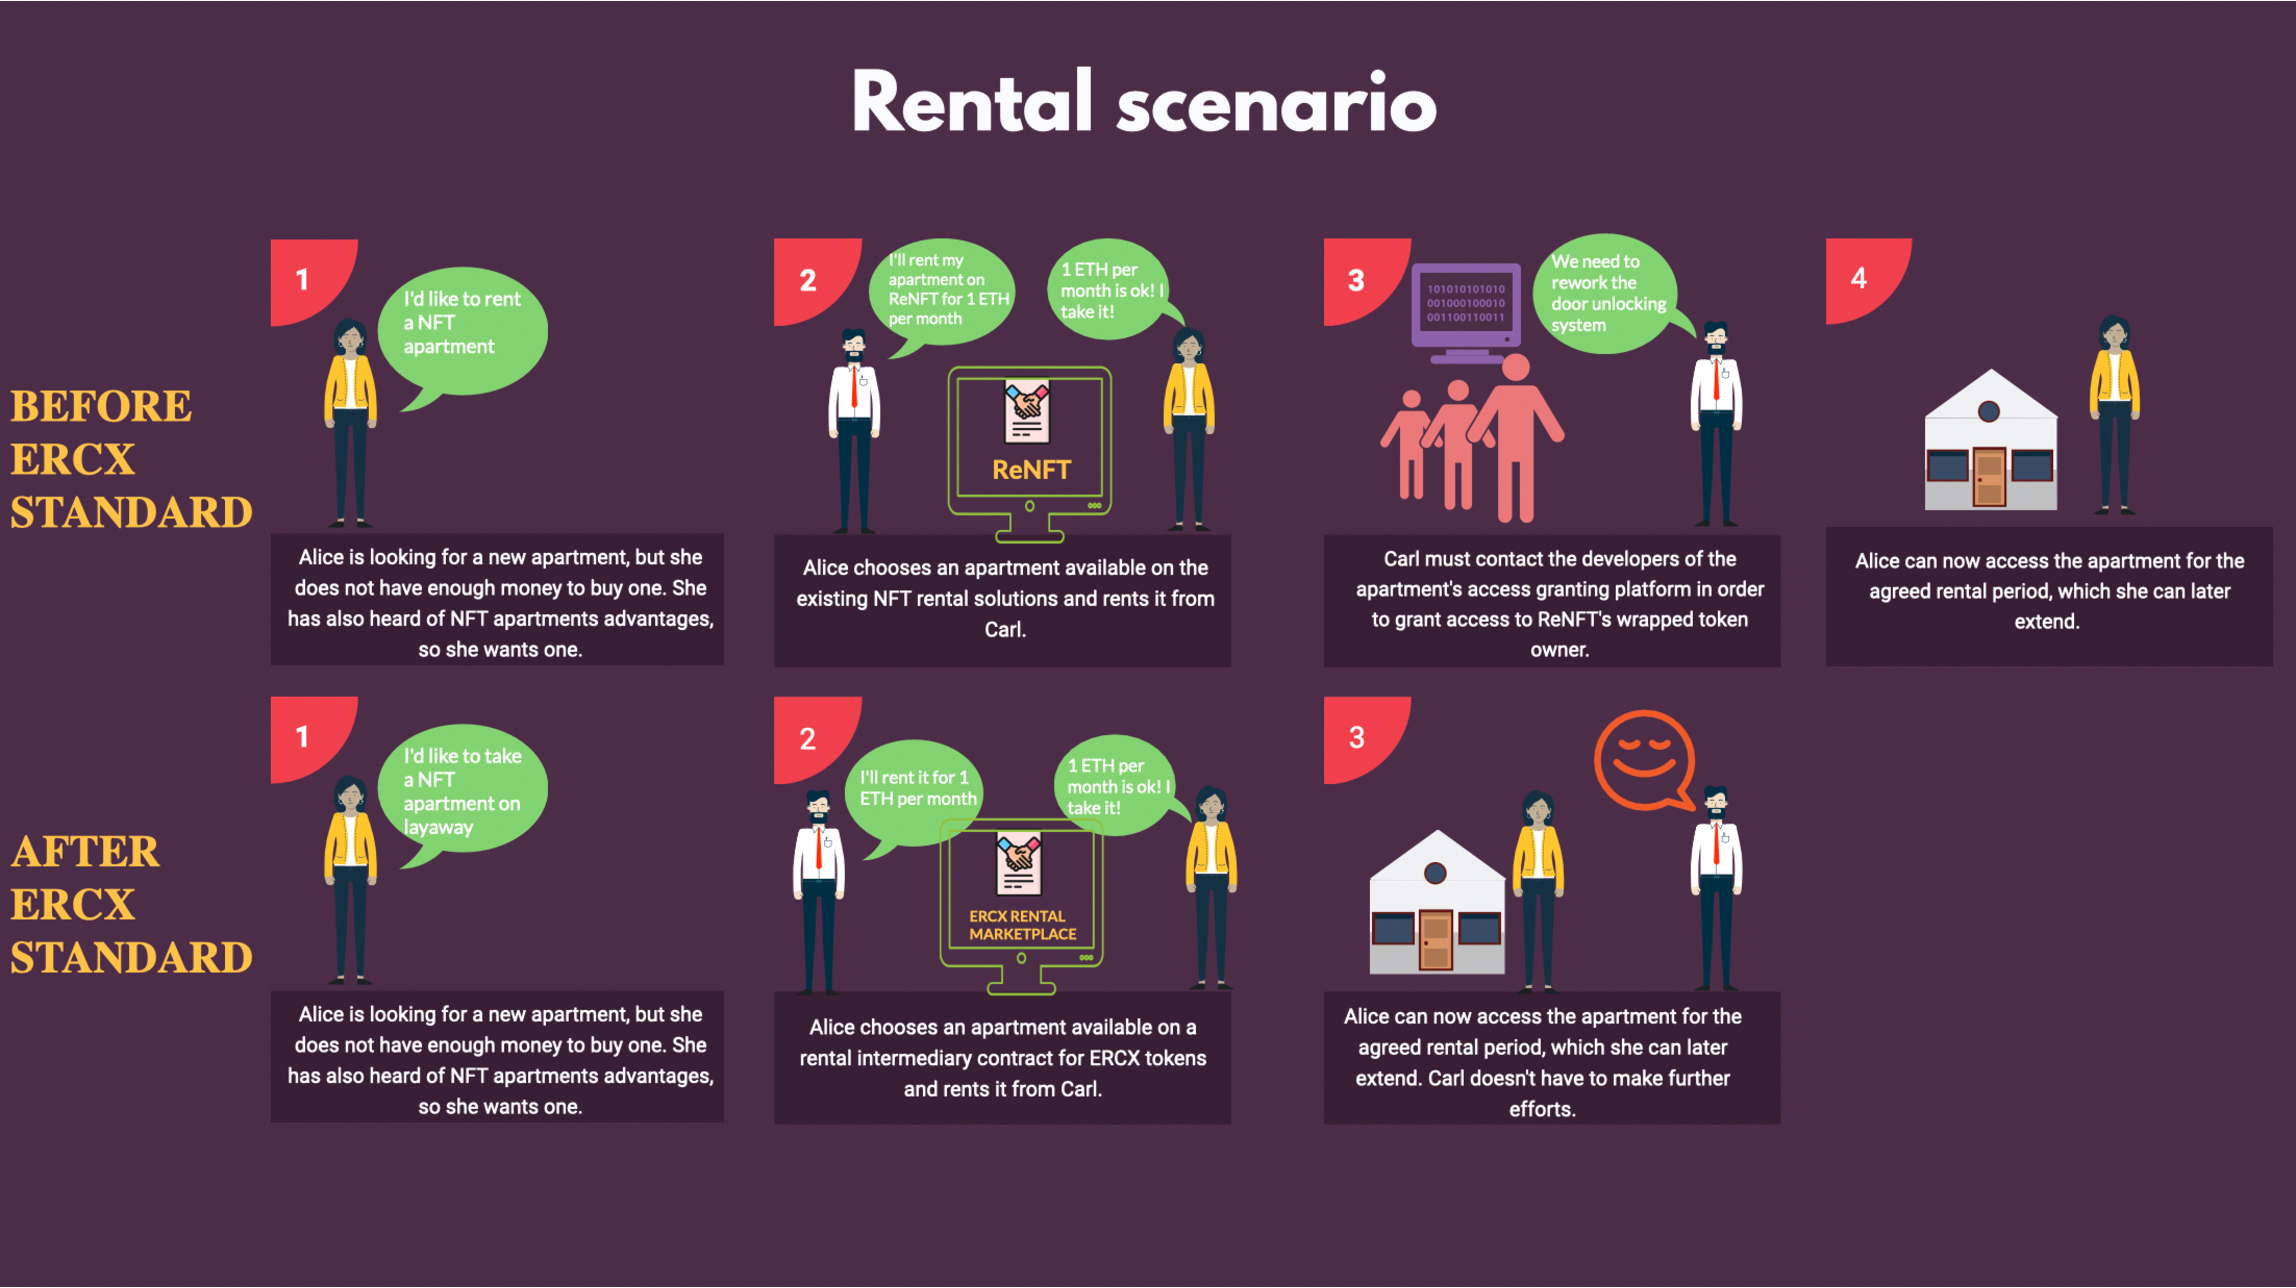
\includegraphics{storyboards/rental.pdf}
        \end{adjustbox}
    \caption{Rental storyboard}
    \label{fig:Rental SB}
\end{figure}

\subsubsection{Subrental}
The storyboard illustrated in Fig.~\ref{fig:Subrental SB} shows how the \textit{escrow-wrap} model does not allow subrental, while the introduction of ERCX standard would enable it. As seen, subrenting capabilities are not always desirable for any type of assets, hence the user who rents a token in the first place will be able to decide to allow of forbid subrental.

\begin{figure}
    \centering
        \begin{adjustbox}{width=1\textwidth}
            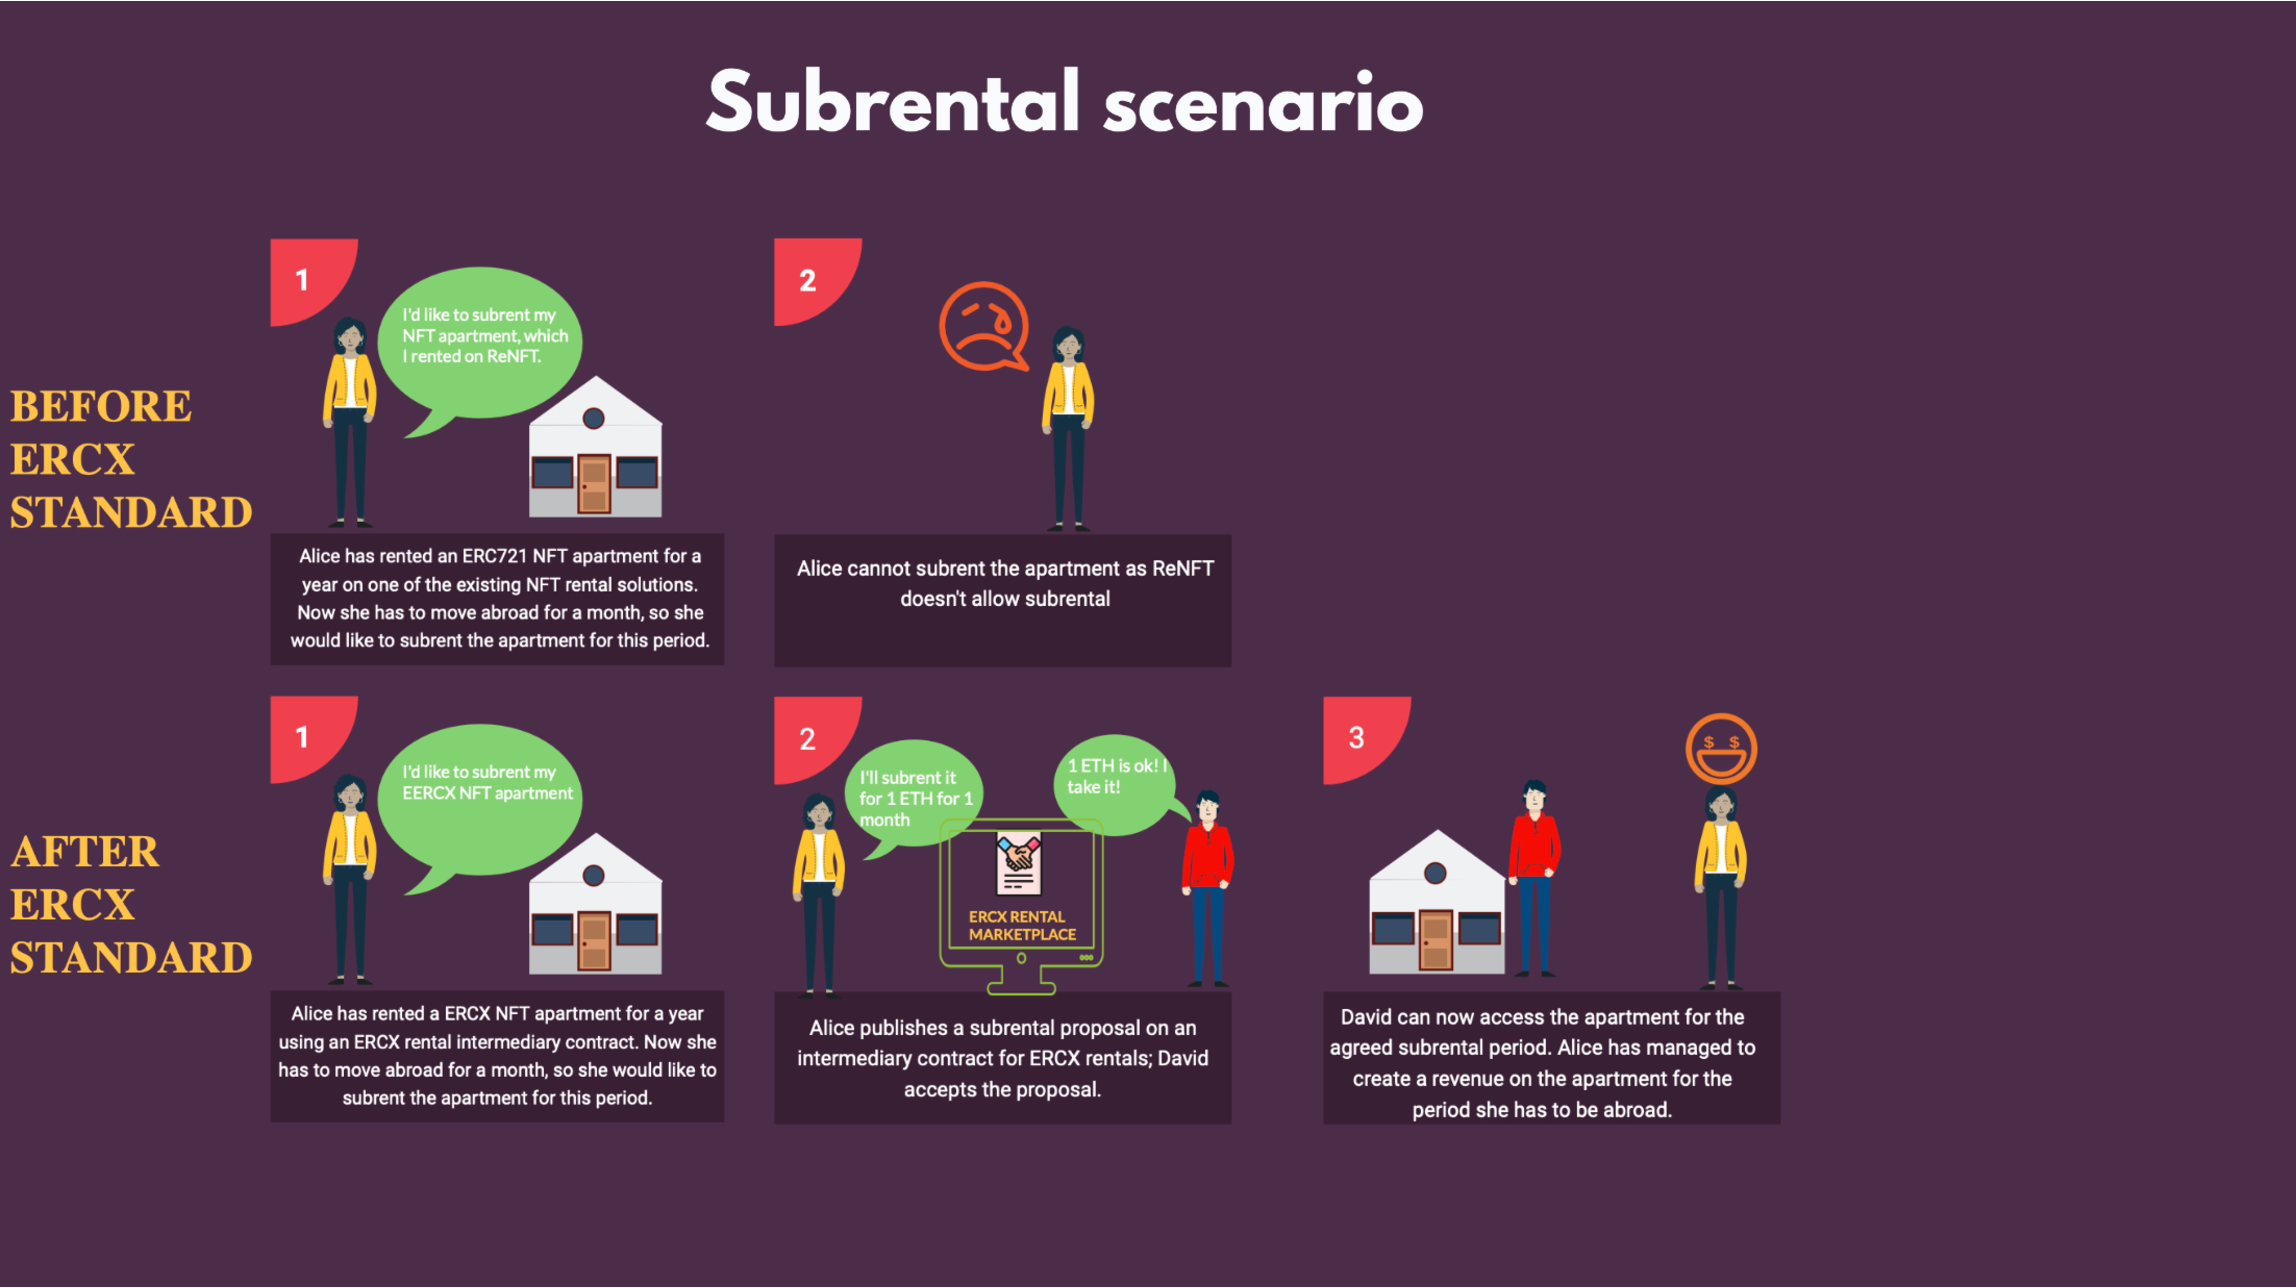
\includegraphics{storyboards/subrental.pdf}
        \end{adjustbox}
    \caption{Subrental storyboard}
    \label{fig:Subrental SB}
\end{figure}

\subsubsection{Rented token transfer}
Moving on to the next storyboard, shown in Fig~\ref{fig:RentedTokenTransfer SB}, we can see how the ability of transferring a rented token can benefit rental receivers, if they don't need or are not able to use the rented token for the whole paid period. In this case, ERCX standard does not introduce this functionality, as it was yet possible to sell wrapped rented tokens, given the existence of a marketplace that supports them. With our proposed solution, on the other hand, this transfer capability is built-in the token architecture, and the provided rental intermediary marketplace reference implementation lets users find a trustless agreement on the transfer price. \newline
In this scenario, we haven't considered the additional burden of adapting the off-chain application to wrapped tokens, as Alice had previously rented the NFT and we assume the adaptation had yet been performed.

\begin{figure}
    \centering
        \begin{adjustbox}{width=1\textwidth}
            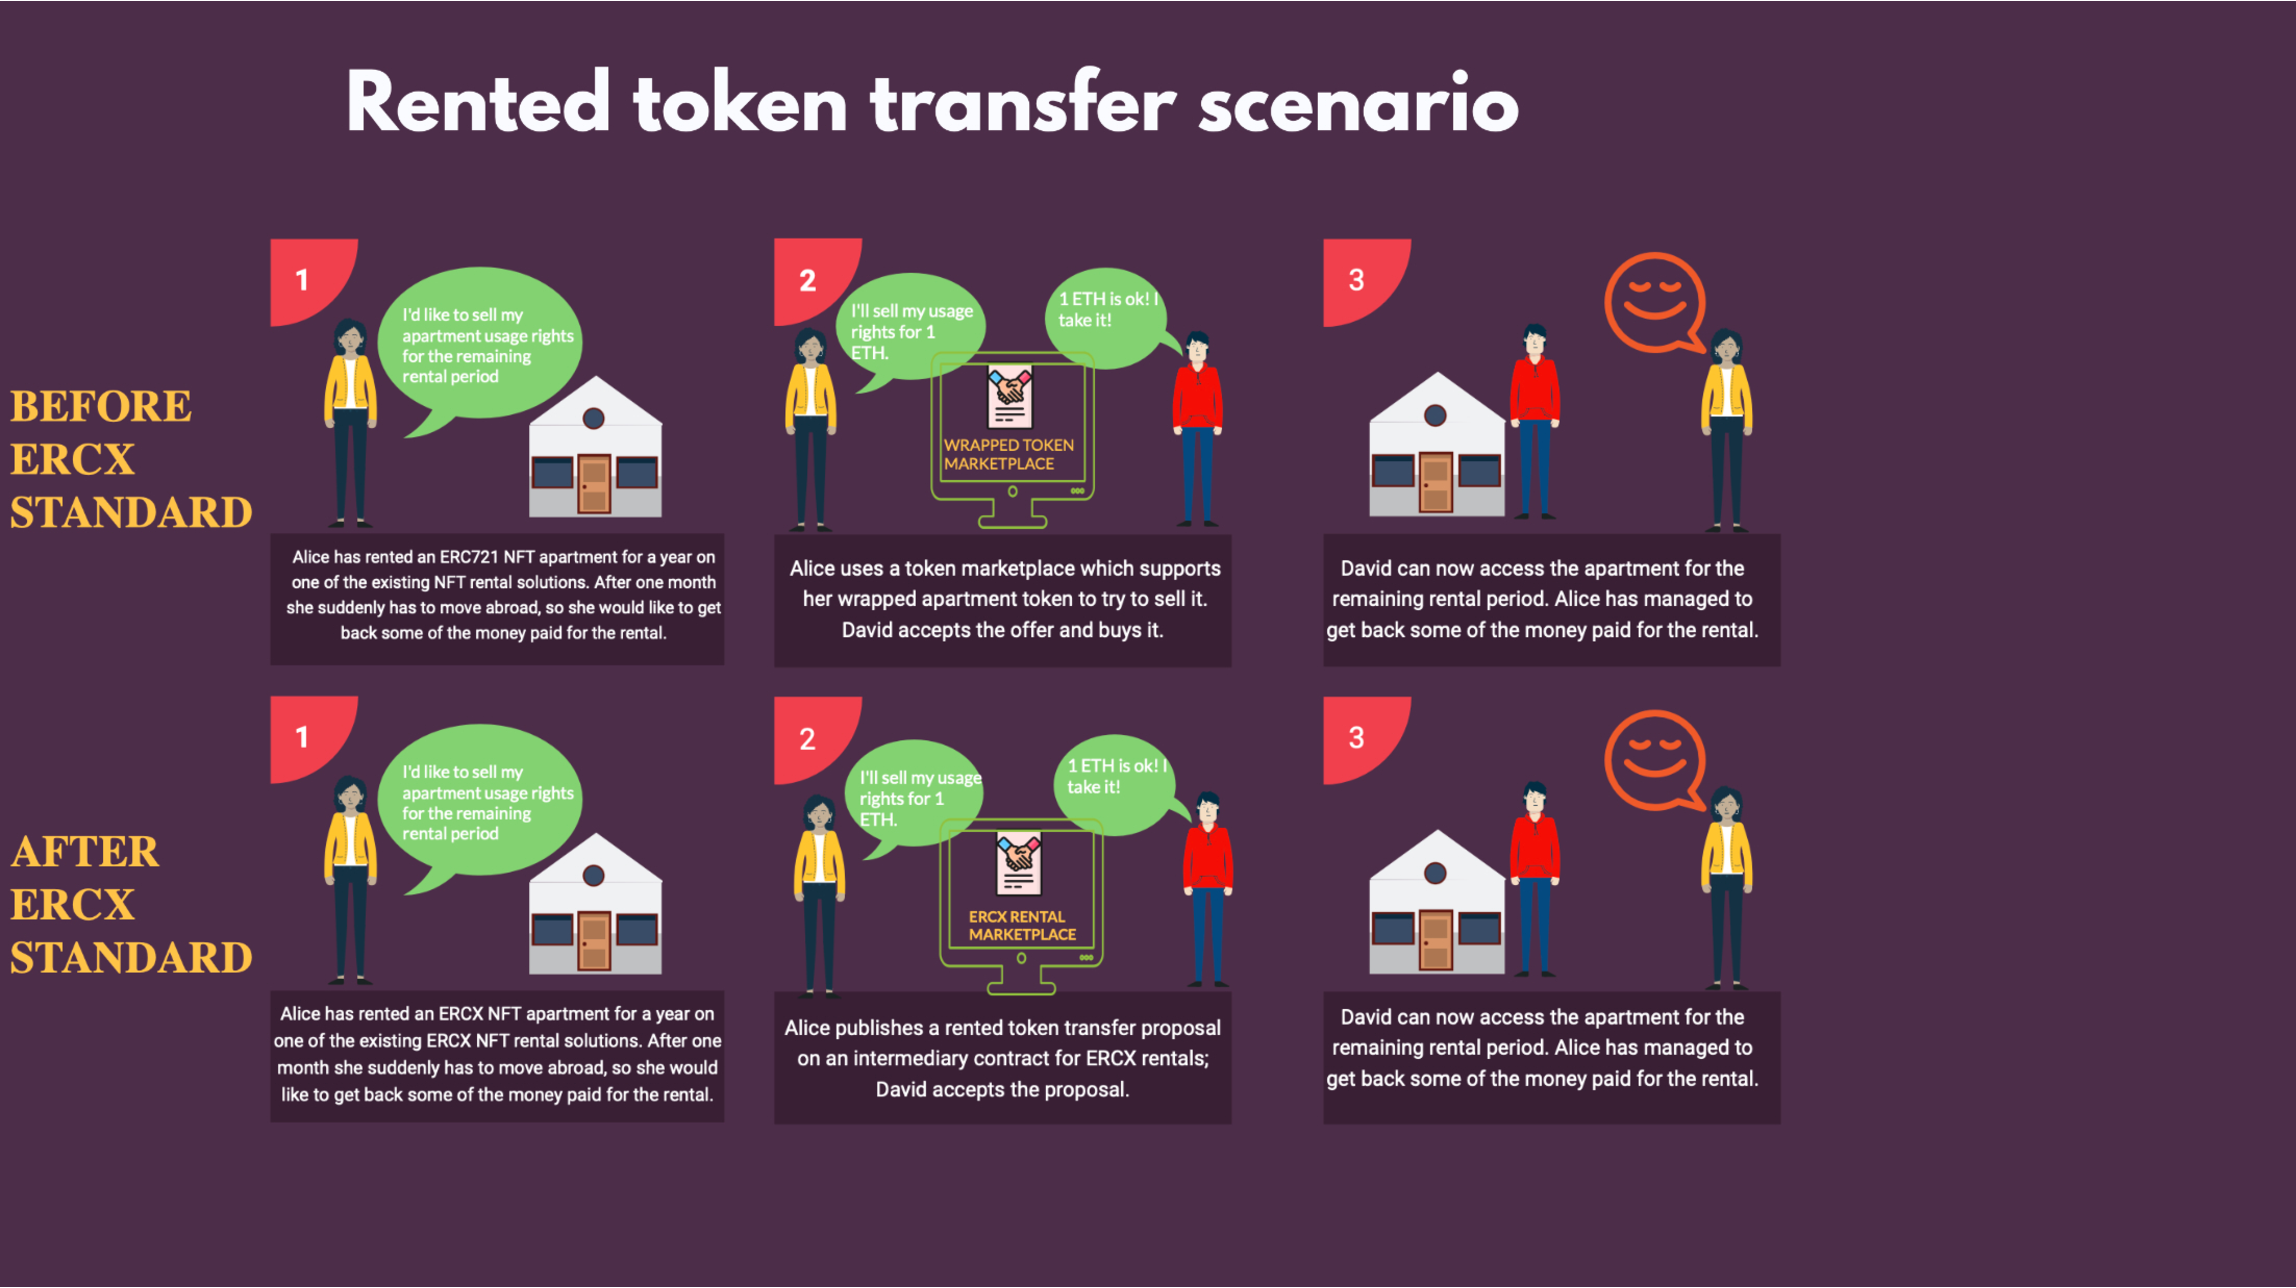
\includegraphics{storyboards/rentedTokenTransfer.pdf}
        \end{adjustbox}
    \caption{Rented token transfer storyboard}
    \label{fig:RentedTokenTransfer SB}
\end{figure}

\subsubsection{Rental ownership transfer}
As introduced before, transfer of rental ownership is the process with which the provider of a rental renounces to the rented token and nominates a new provider; the new provider will get the token back at the end of the rental, and also further rental extension payments, if any. As all the others, this operation can be performed using the provided ERCX intermediary rental marketplace. \newline
As shown in the Fig.~\ref{fig:RentalOwnershipTransfer SB}, this feature can be useful when a rental provider suddenly needs some liquidity, enabling them to sell the rented token even if rental period is not expired.\newline
This functionality was not available with \textit{escrow-wrap} rental.

\begin{figure}
    \centering
        \begin{adjustbox}{width=1\textwidth}
            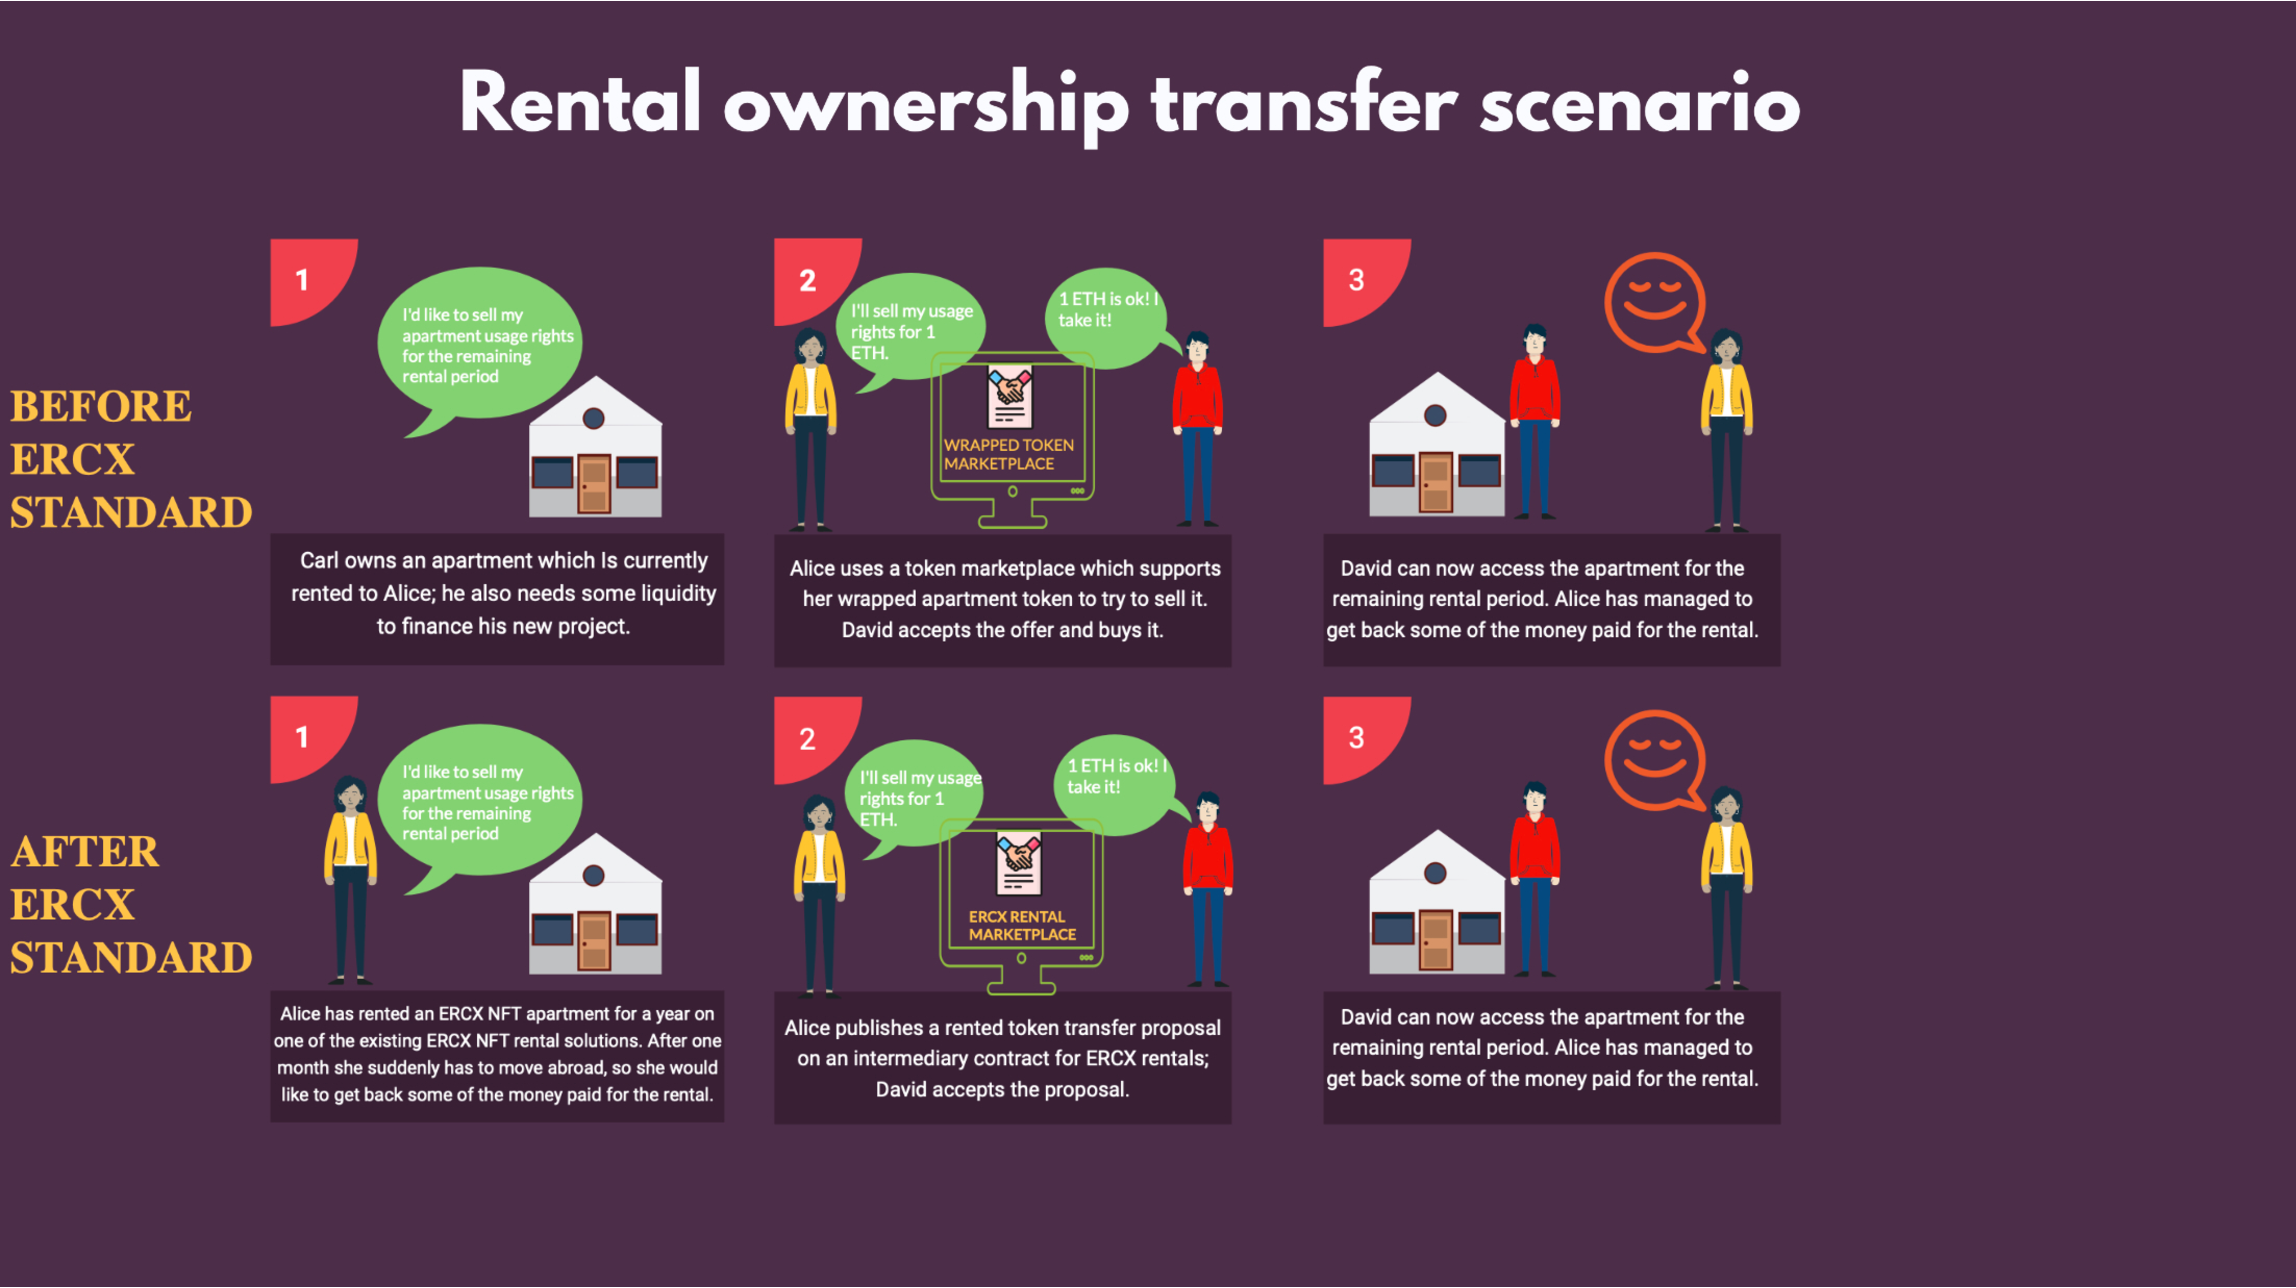
\includegraphics{storyboards/rentalTransfer.pdf}
        \end{adjustbox}
    \caption{Rental ownership transfer storyboard}
    \label{fig:RentalOwnershipTransfer SB}
\end{figure}

\subsubsection{Rented token redemption}
\begin{figure}[H]
    \centering
        \begin{adjustbox}{width=1\textwidth}
            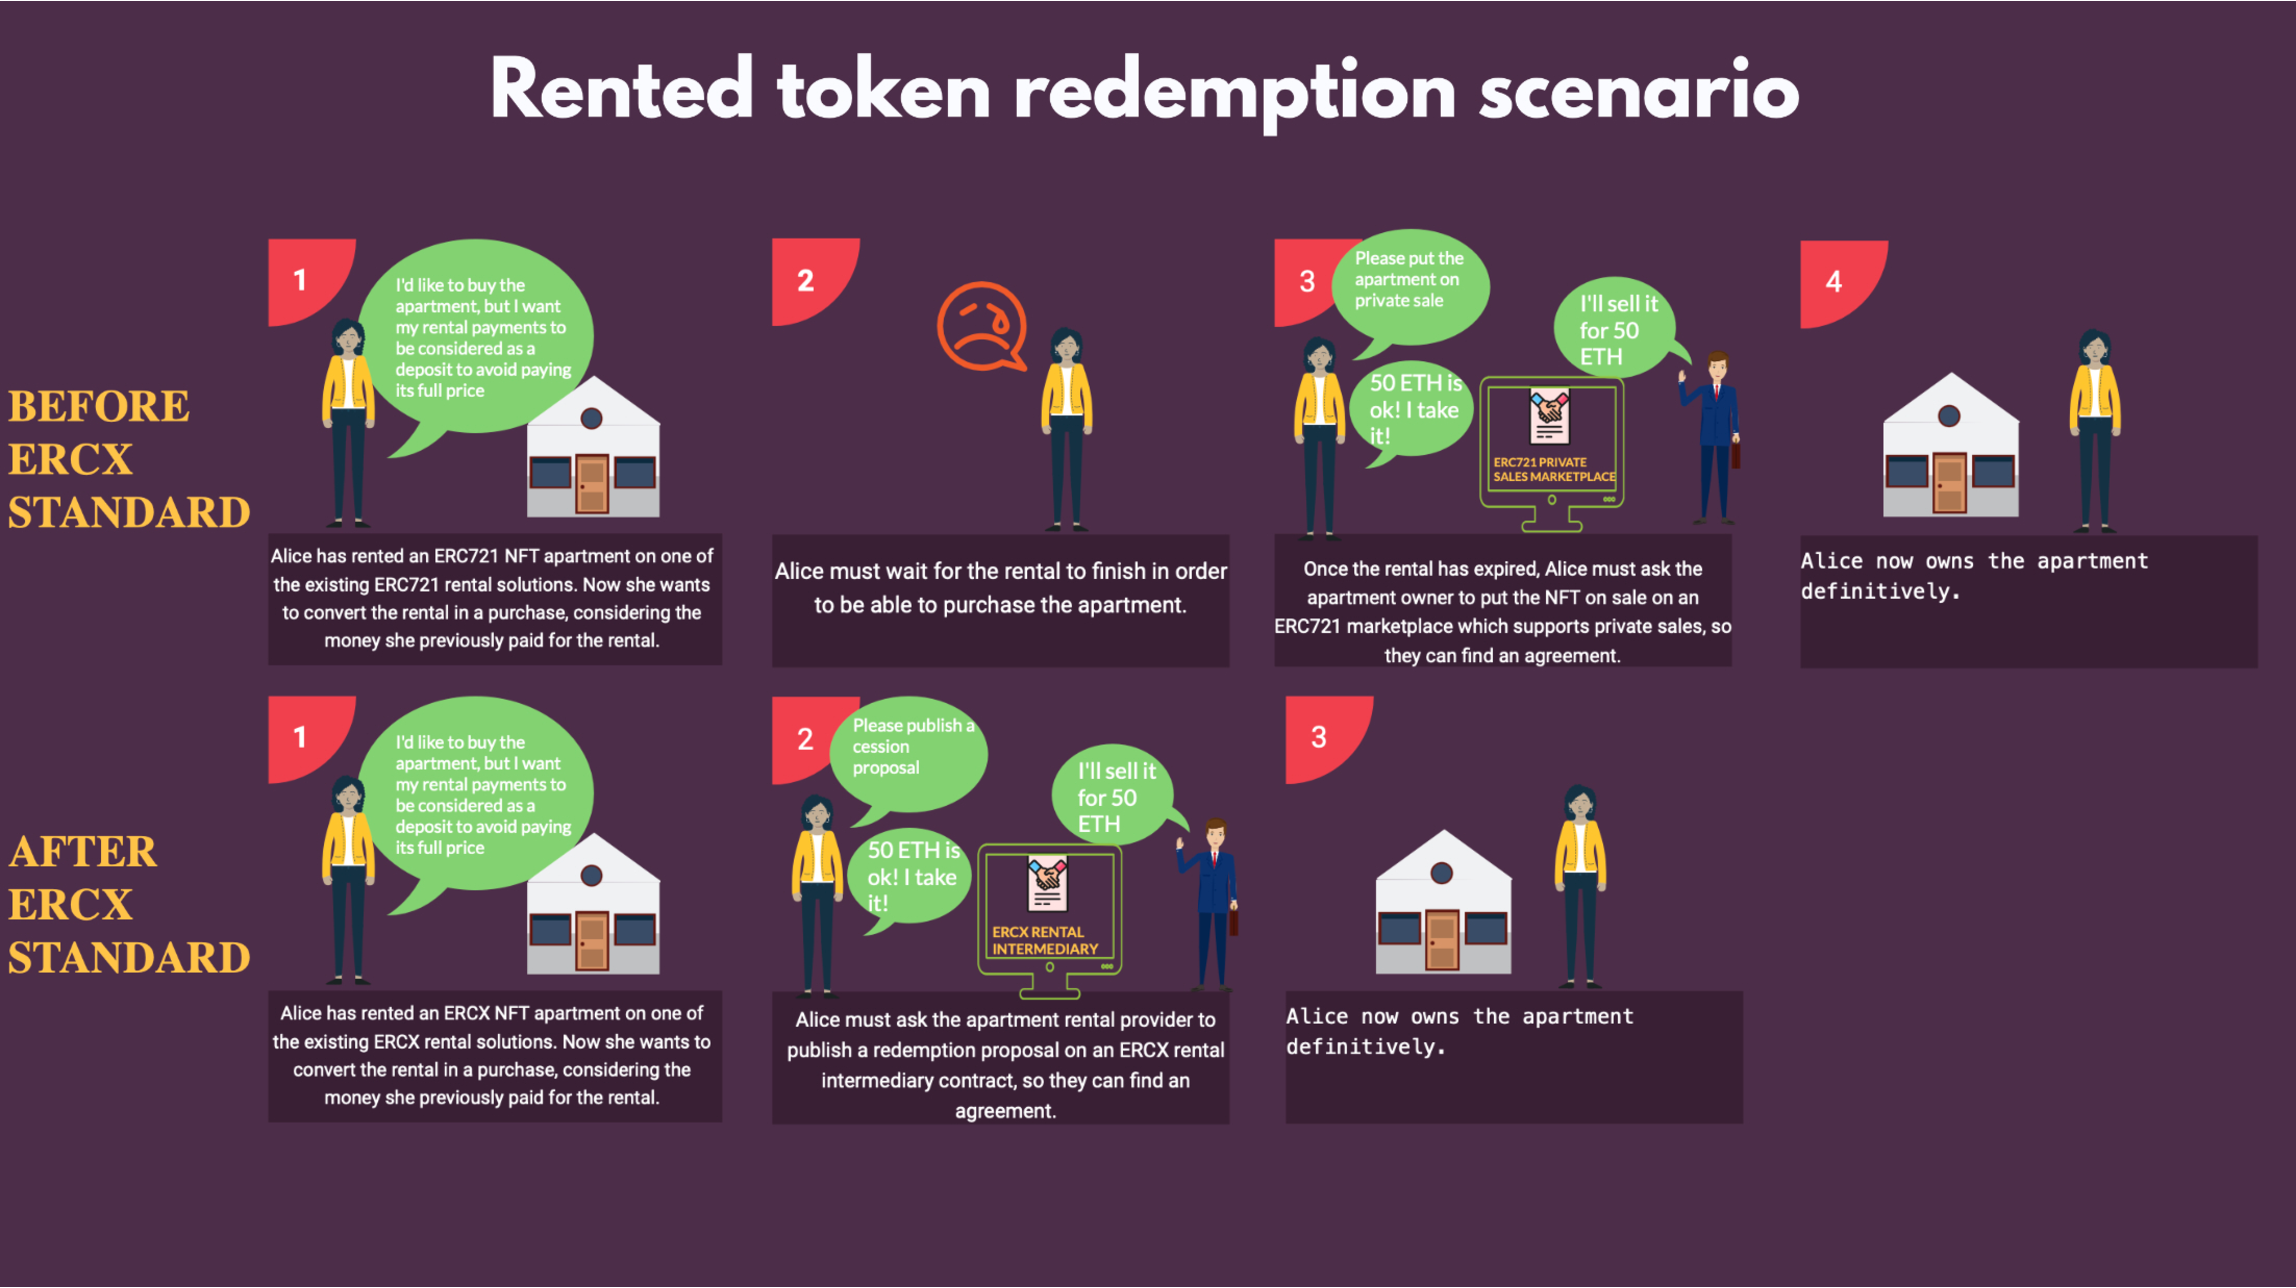
\includegraphics{storyboards/rentedTokenRedemption.pdf}
        \end{adjustbox}
    \caption{Rented token redemption storyboard}
    \label{fig:RentedTokenRedemption SB}
\end{figure}

Another functionality introduced by ERCX tokens is the redemption of a rented token by the rental receiver during the rental period. 
This feature is very often used in the real world; as Fig.~\ref{fig:RentedTokenRedemption SB} depicts, if the rental receiver wants to definitively purchase the asset he is renting, they can find an agreement with the provider for a redemption price, which will probably take past rental payments into account.
This agreement can be again reached using the provided rental intermediary marketplace reference implementation.


\subsubsection{Layaway}

Moving on to layaway, as depicted by Fig.~\ref{fig:Layaway SB}, the advantages introduced by ERCX tokens usage are quite similar to the ones discussed for rental. Again, renting an ERC721 token using the \textit{escrow-wrap} approach implies having to adapt the off-chain system that assigns tokens' usage rights to also check the wrapped token's ownership.

\begin{figure}[H]
    \centering
        \begin{adjustbox}{width=1\textwidth}
            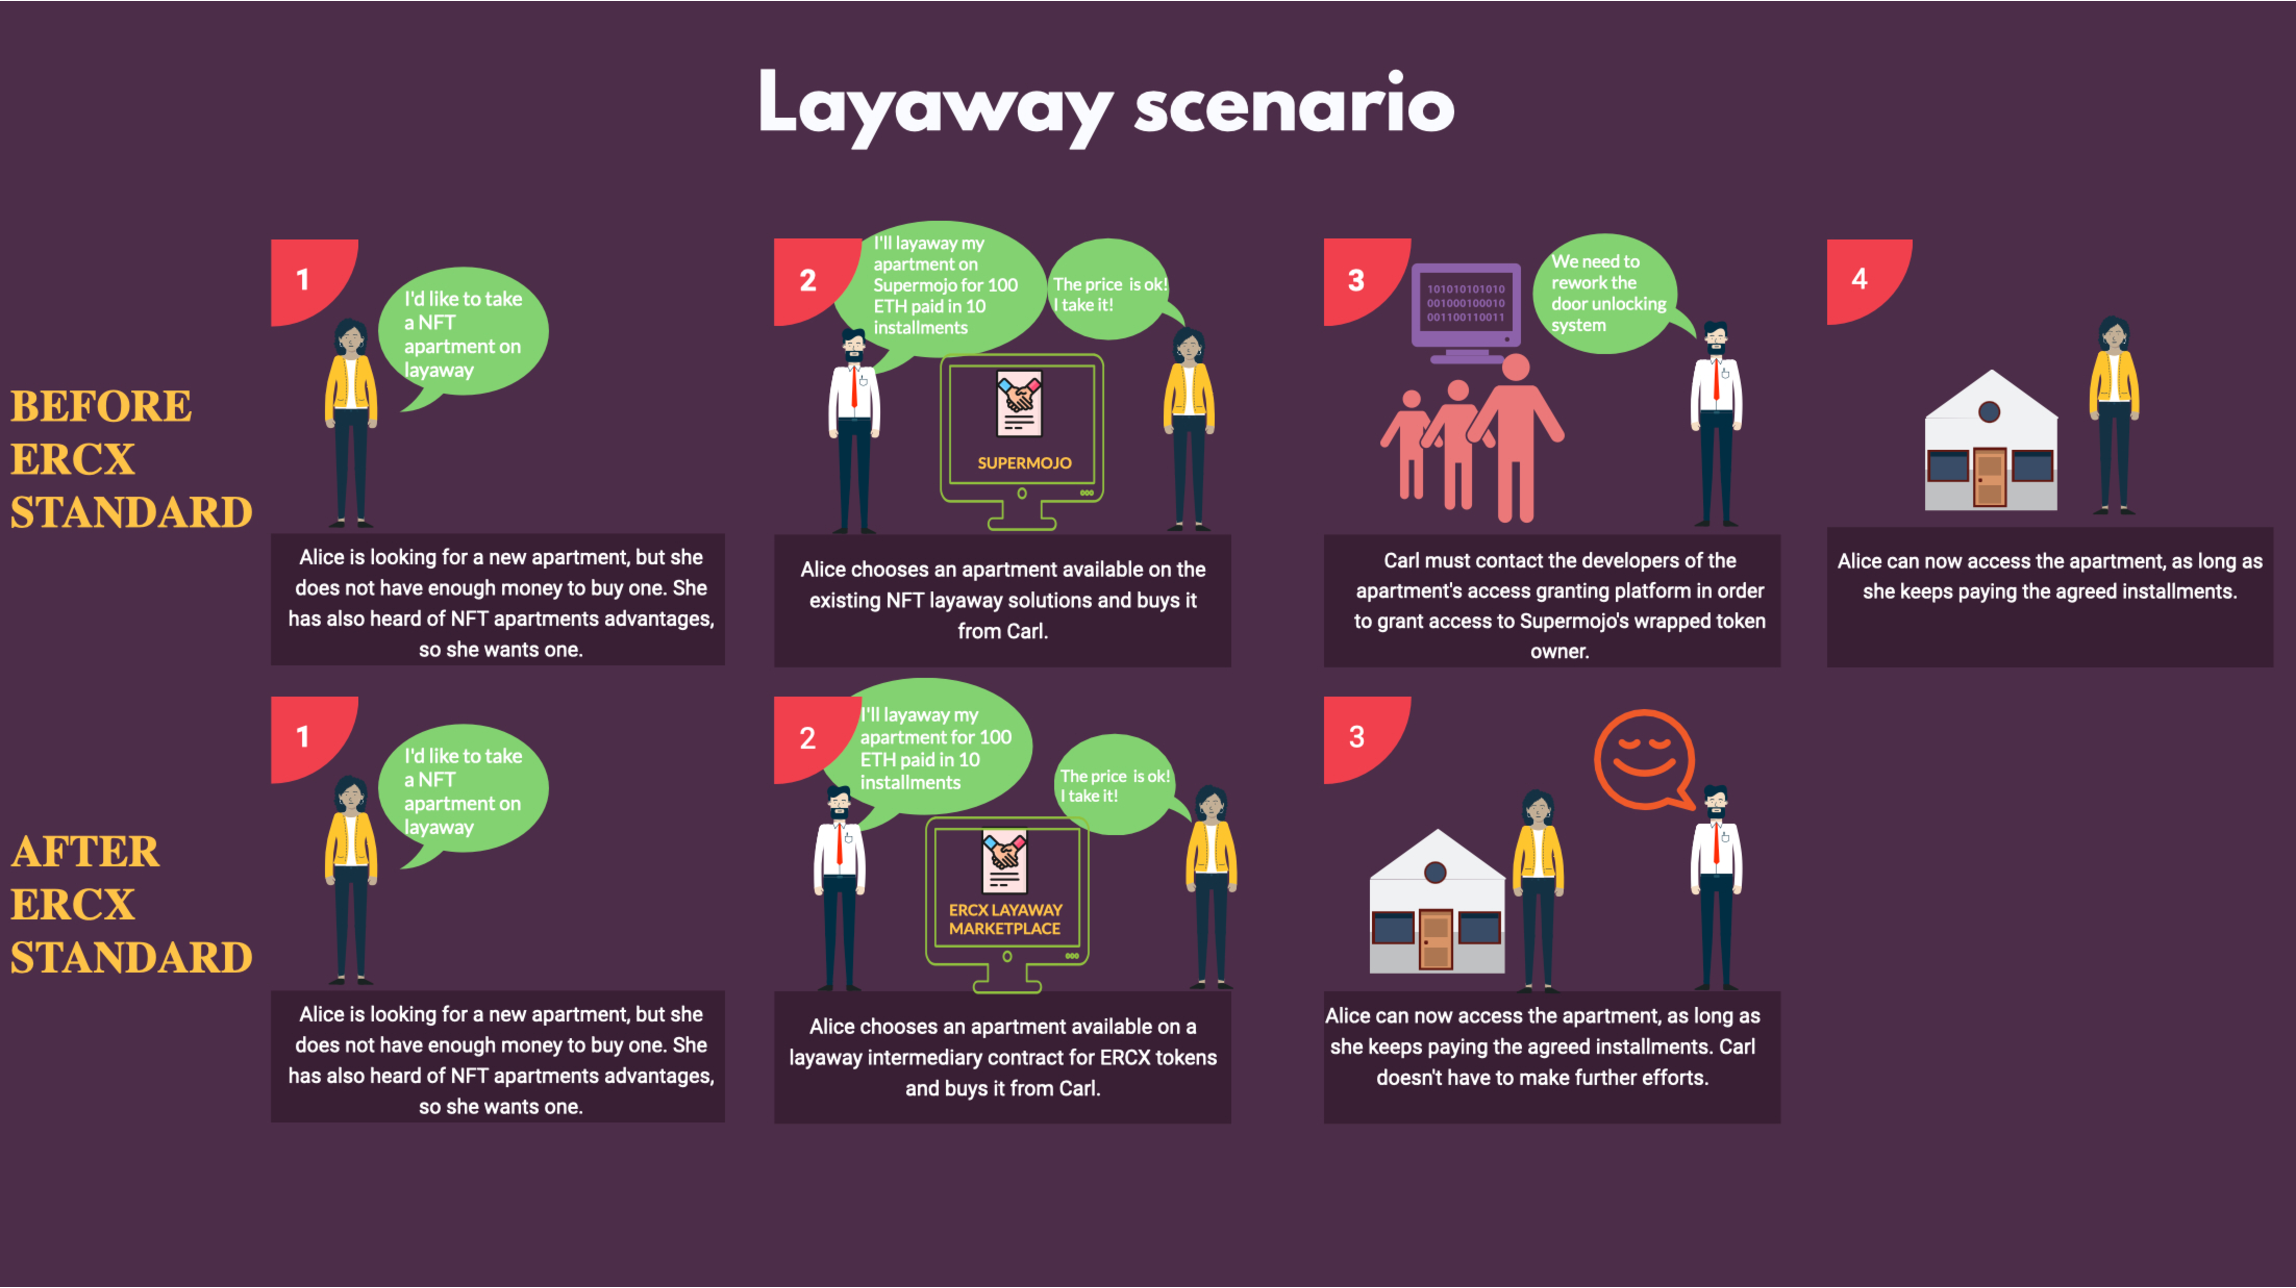
\includegraphics{storyboards/layaway.pdf}
        \end{adjustbox}
    \caption{Layaway storyboard}
    \label{fig:Layaway SB}
\end{figure}



\subsubsection{Layawayed token transfer}

Transferring a token during a layaway is in some sense similar to transferring a rented token. In particular, when the transfer happens, the receiver of the layaway is changed to a new one, who will have to pay the remaining installments in order to keep the token at the end of the layaway. \newline
As seen for rental, Fig.~\ref{fig:LayawayedTokenTransfer SB} shows how this feature could also be accomplished with the existing \textit{escrow-wrap} ERC721 layaway solutions. Again, the provided ERCX layaway intermediary contract reference implementation lets users find an agreement on the price and perform the transfer.

\begin{figure}[H]
    \centering
        \begin{adjustbox}{width=1\textwidth}
            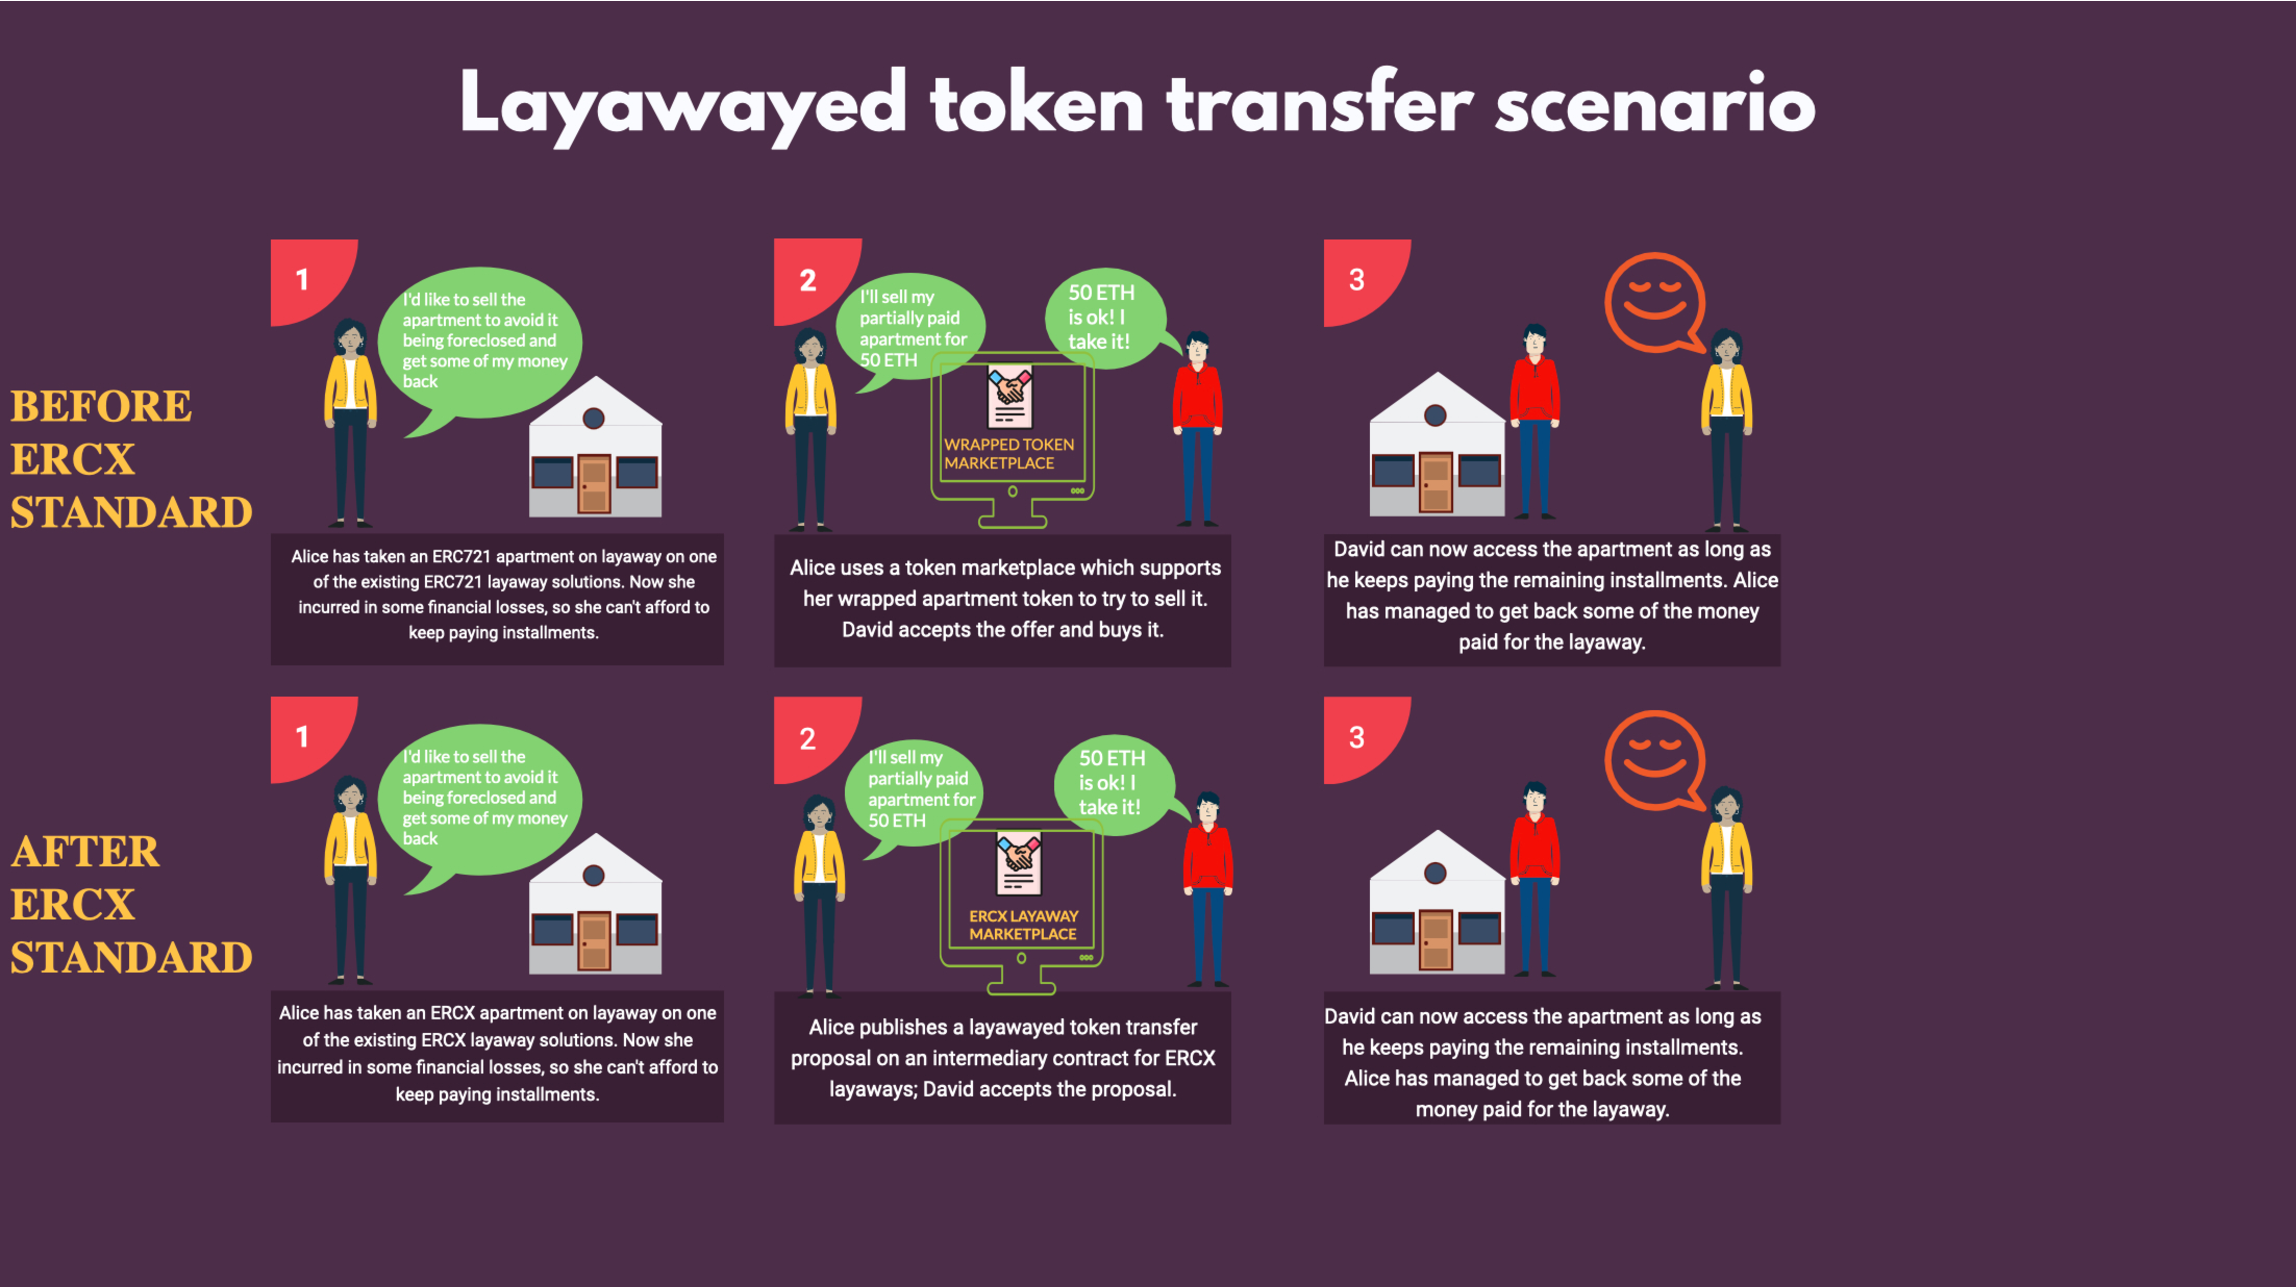
\includegraphics{storyboards/layawayedTokenTransfer.pdf}
        \end{adjustbox}
    \caption{Layawayed token transfer storyboard}
    \label{fig:LayawayedTokenTransfer SB}
\end{figure}


\subsubsection{Layaway ownership transfer}
Layaway ownership transfer is the process with which the provider of a layaway can immediately sell a token under layaway and make an immediate revenue out of it, without having to wait all the installments payments. This is clearly shown in the storyboard (Fig.~\ref{fig:LayawayOwnershipTransfer SB}), which also shows how this type of functionality was not available for \textit{escrow-wrap} layaways. \newline
Once more, the responsibility of letting users find an agreement on transfer price and starting the transfer can be assigned to the provided ERCX layaway intermediary marketplace contract.

\begin{figure}[H]
    \centering
        \begin{adjustbox}{width=1\textwidth}
            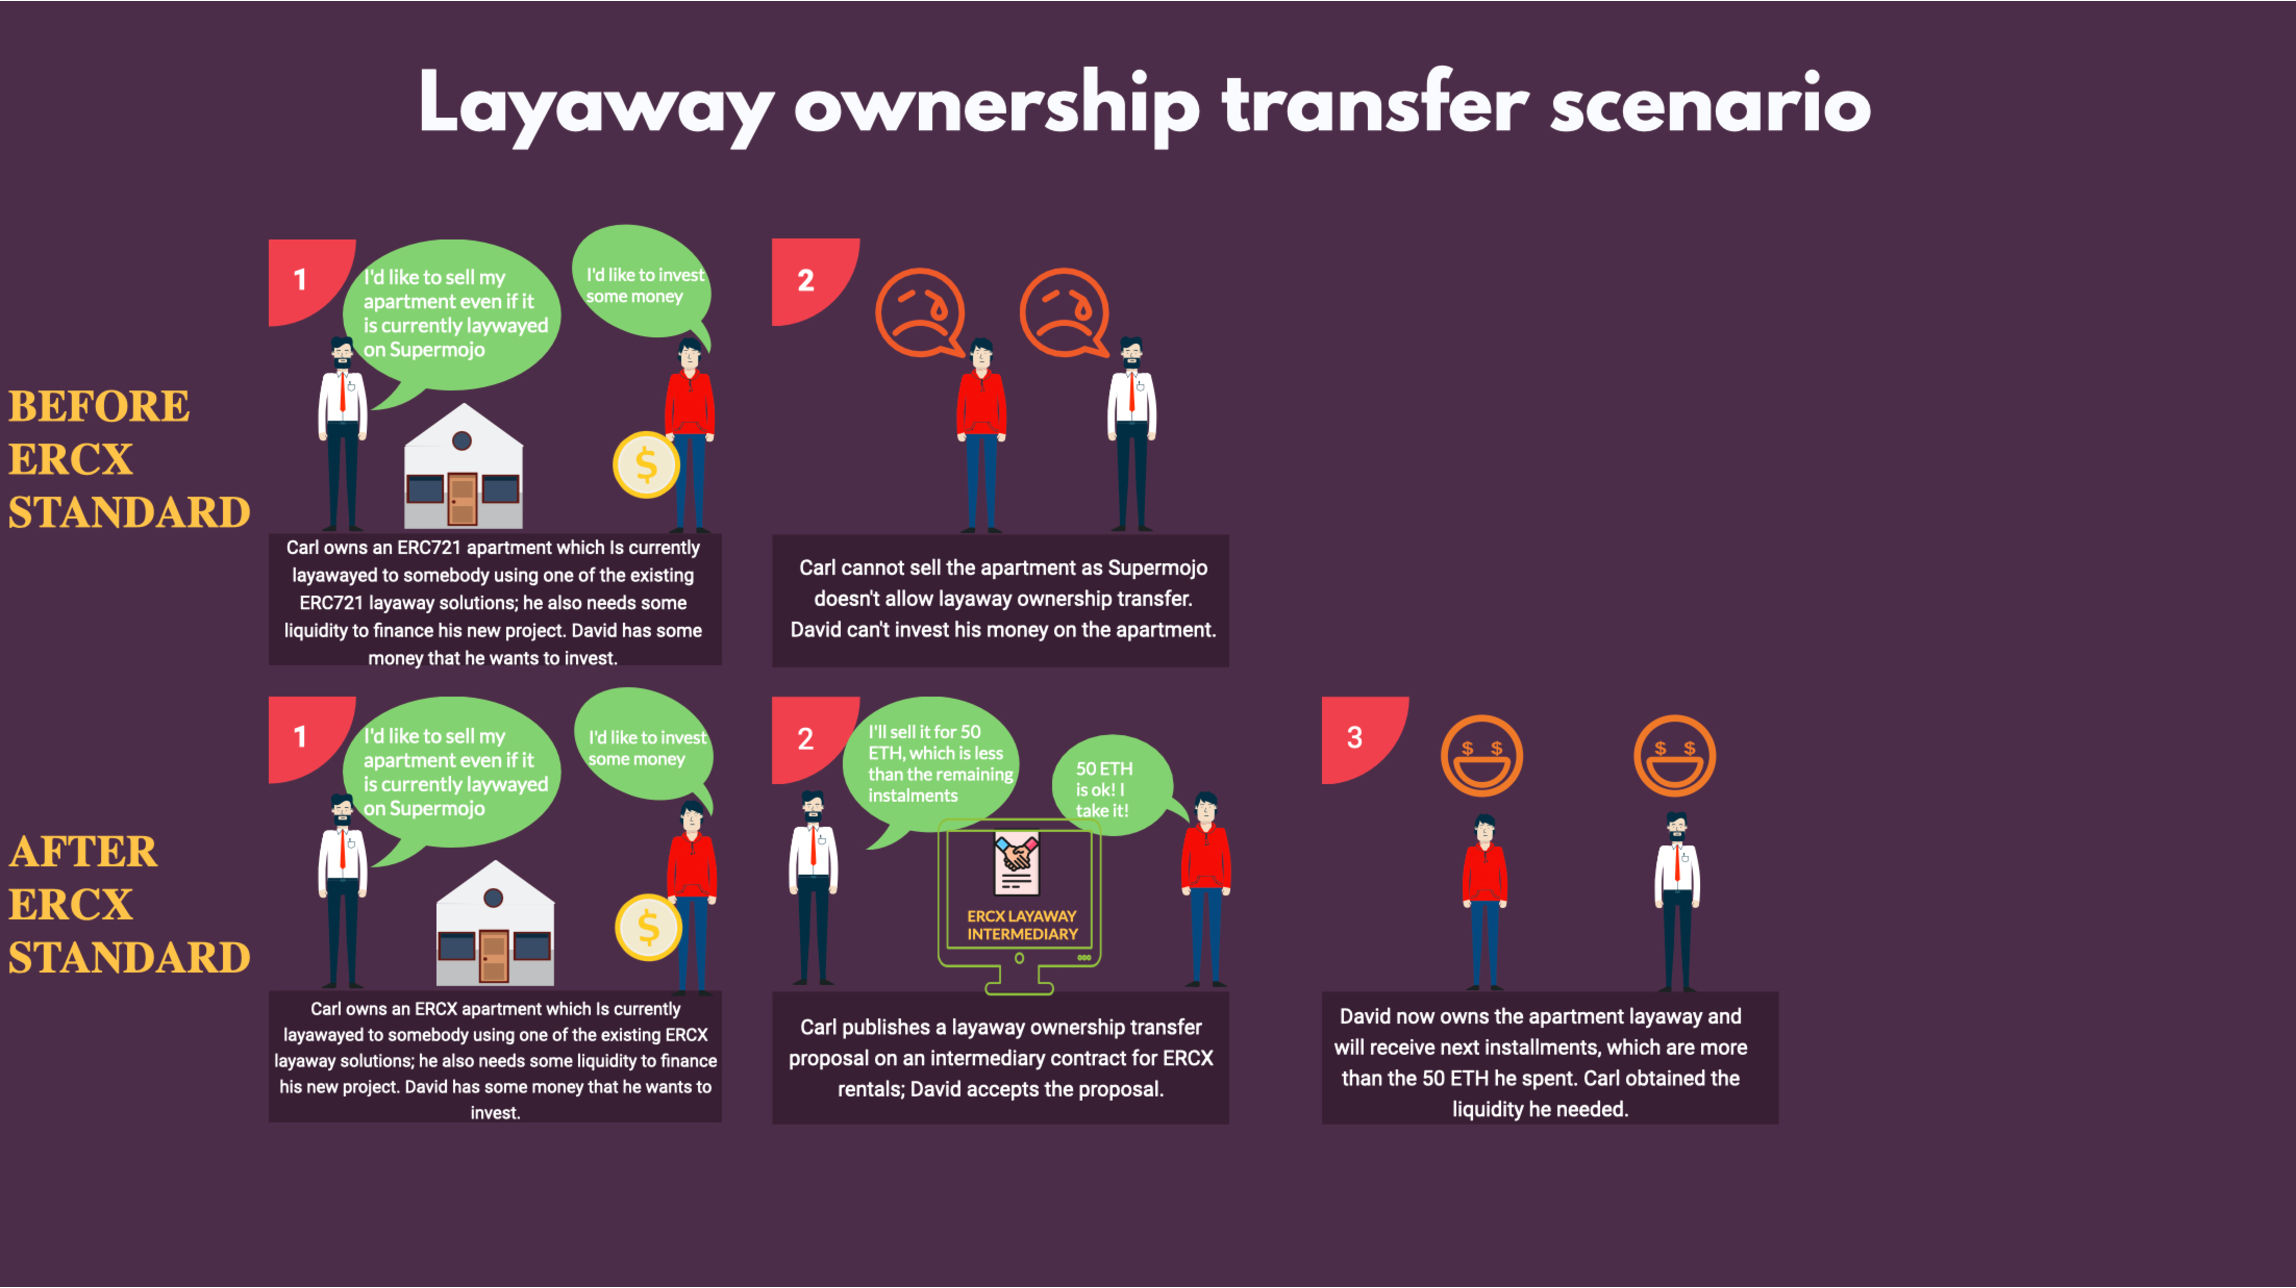
\includegraphics{storyboards/layawayTransfer.pdf}
        \end{adjustbox}
    \caption{Layaway ownership transfer storyboard}
    \label{fig:LayawayOwnershipTransfer SB}
\end{figure}

\subsection{Use cases diagram}

\begin{figure}
    \centering
        \begin{adjustbox}{width=1\textwidth}
            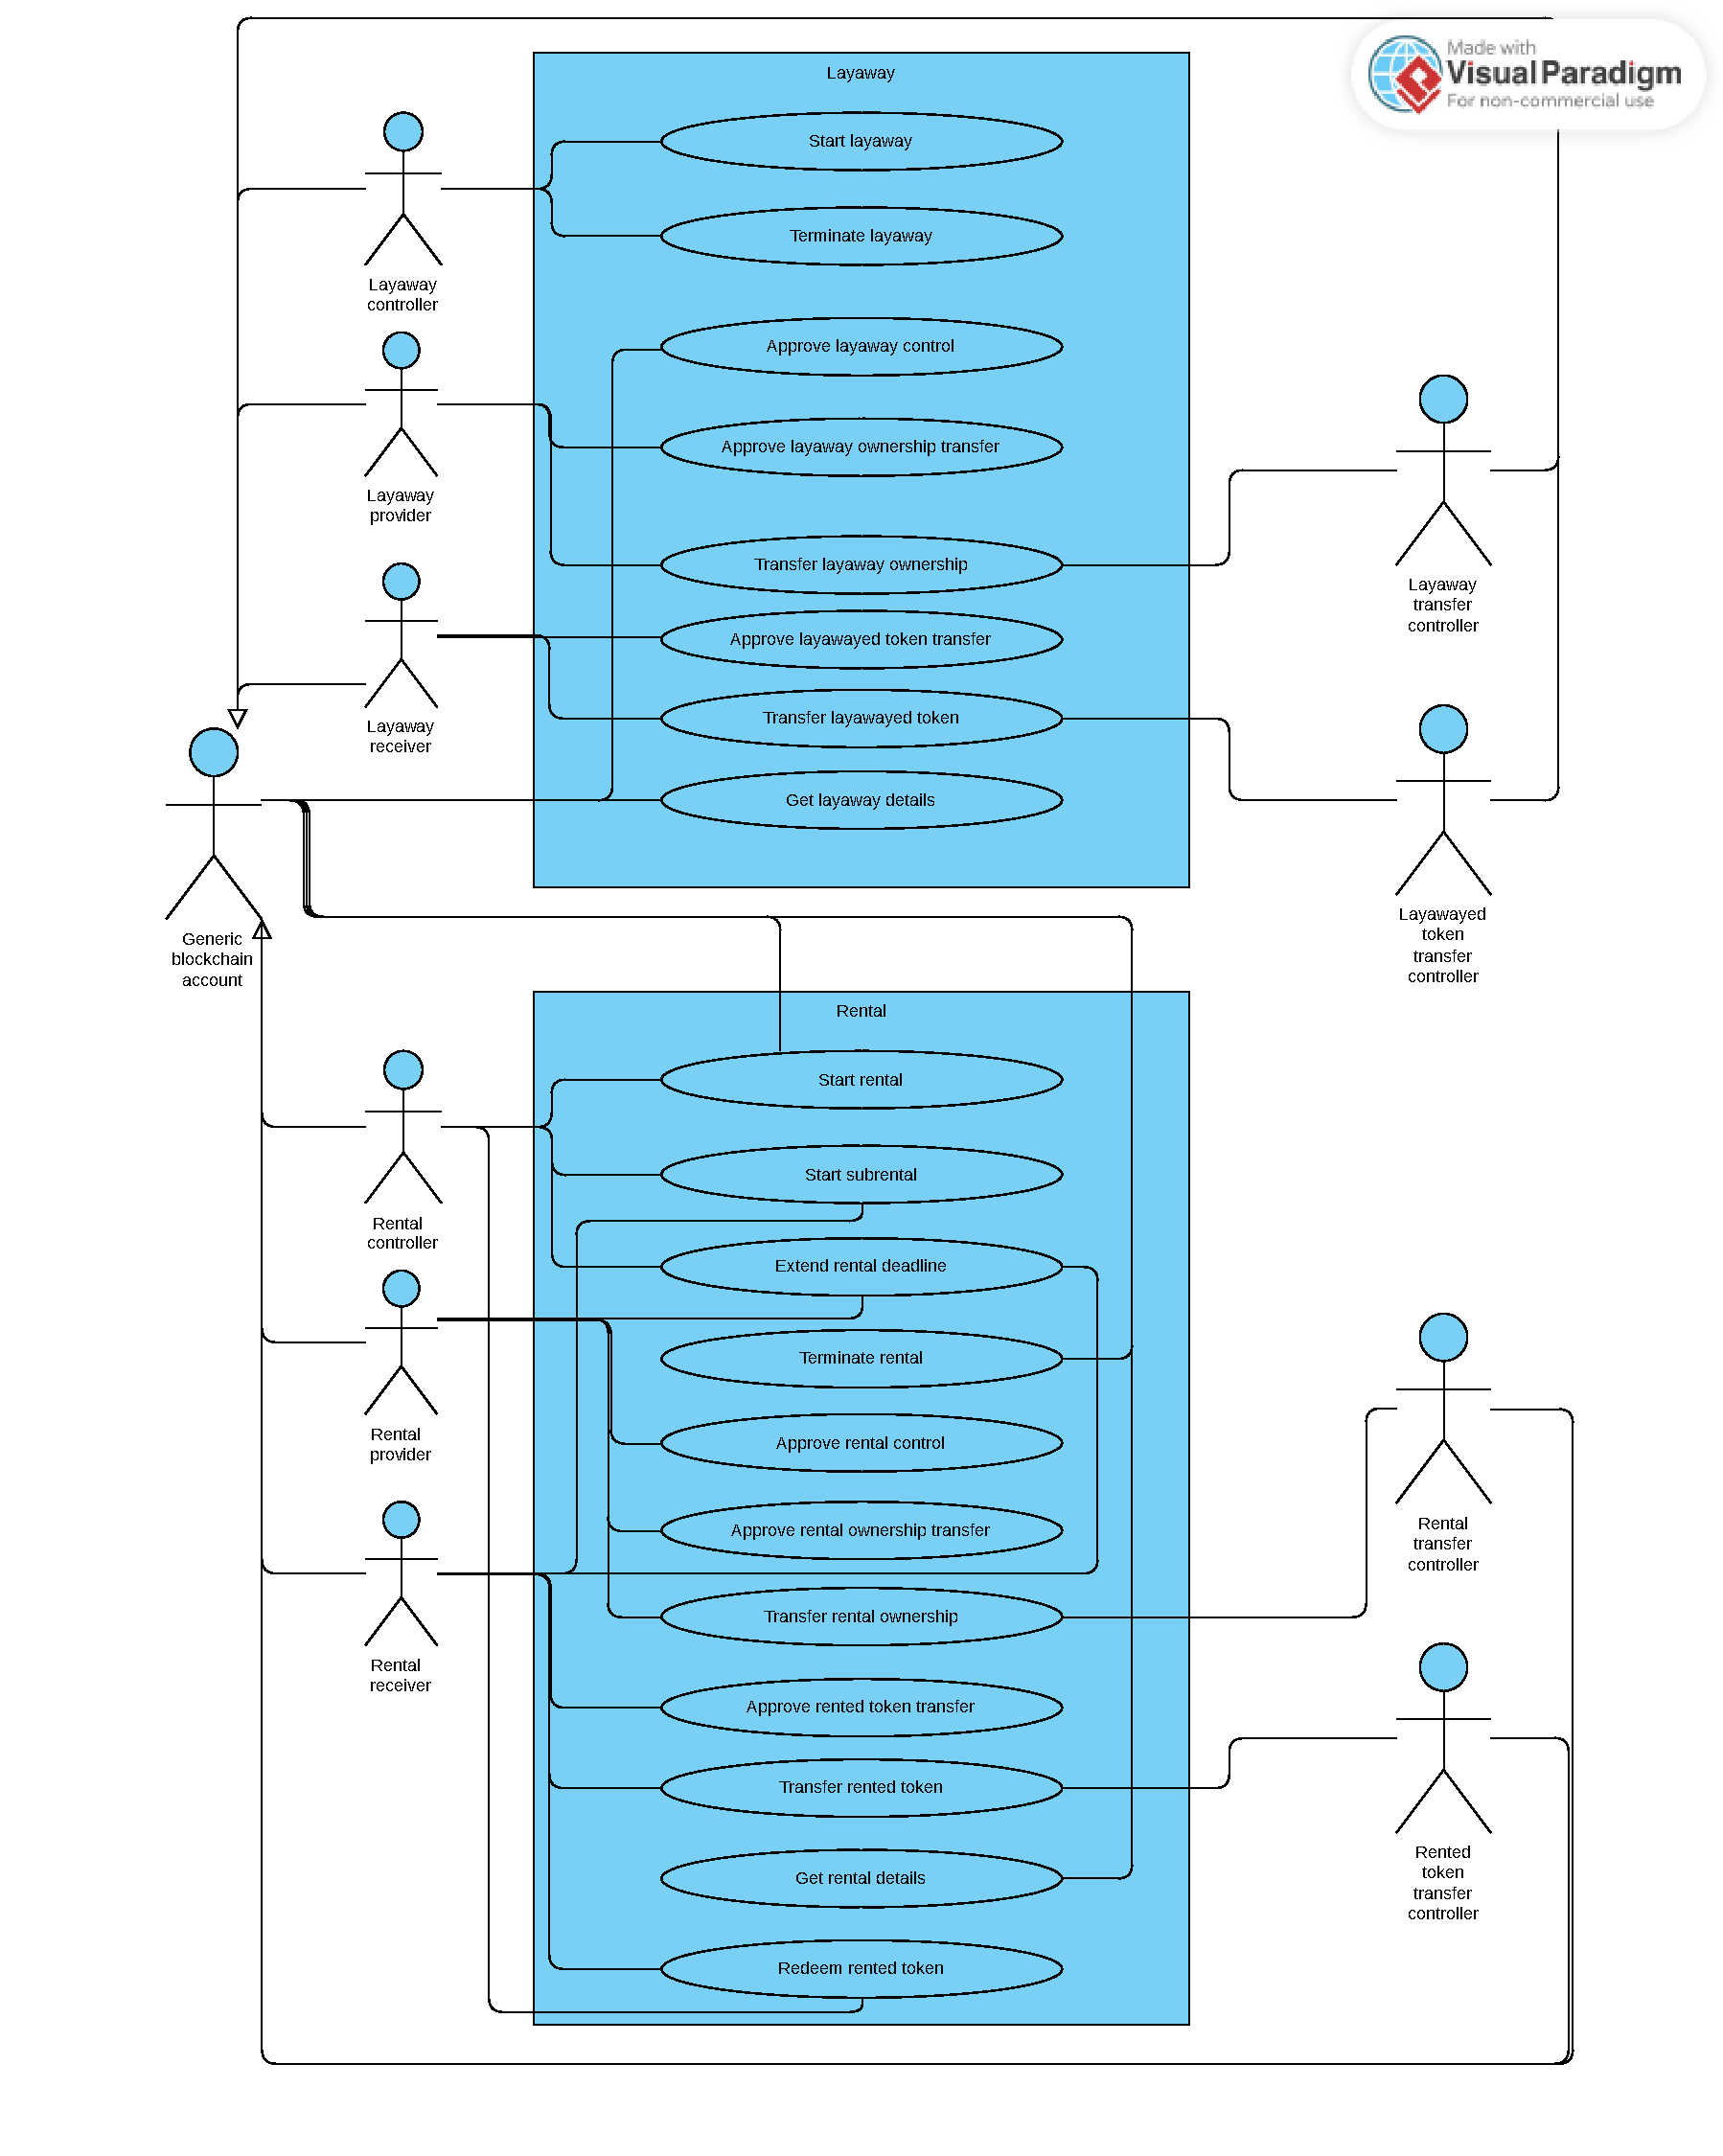
\includegraphics{UseCasesDiagrams/useCaseDiagram.pdf}
        \end{adjustbox}
    \caption{Use cases diagram}
    \label{fig:UseCaseDiagram}
\end{figure}

Next diagram to be discussed is the use cases diagram, shown in Fig.~\ref{fig:UseCaseDiagram}. This type of diagram is defined in UML and has been created using UML notation, as for the next diagrams that will be shown.
It  shows which are the actors who interact with the system and what functionalities each of them can use. The most generic actor is the generic blockchain account, which is extended by all the other actors that appear in the diagram. Rental and layaway providers are the users who respectively rent out and sell on layaway their tokens, while receivers are the ones who receive the tokens on rent and layaway. Rental and layaway controllers are instead the accounts nominated as rental and layaway intermediaries, needed for the reasons discussed in the previous sections. Finally, rental and layaway transfer controllers are the intermediaries used to perform rental and layaway ownership transfer, while rented token and layawayed token transfer controllers are the intermediaries used to transfer tokens during rental and layaway.



\subsection{Activity diagrams}
Having analyzed and understood all the system's use cases, we can now move on to describe more specifically the ERCX token's lifecycle and the processes that enable the discussed functionalities. This is the purpose of the following UML activity diagrams, each of which will be discussed separately.

\subsubsection{Rental}

This first diagram (Fig.~\ref{fig:Rental AD}) shows how a rental can be started and terminated. As previously discussed, it can be done both with and without using an intermediary, which can be an EOA or a smart contract. The only other elements worth commenting are the "Is rental valid" decisional points: their purpose is to check various conditions on the proposed rental, such as the token not being currently rented or layawayed and that the rental has not expired yet. 

\begin{figure}[H]
    \centering
        \begin{adjustbox}{width=1\textwidth}
            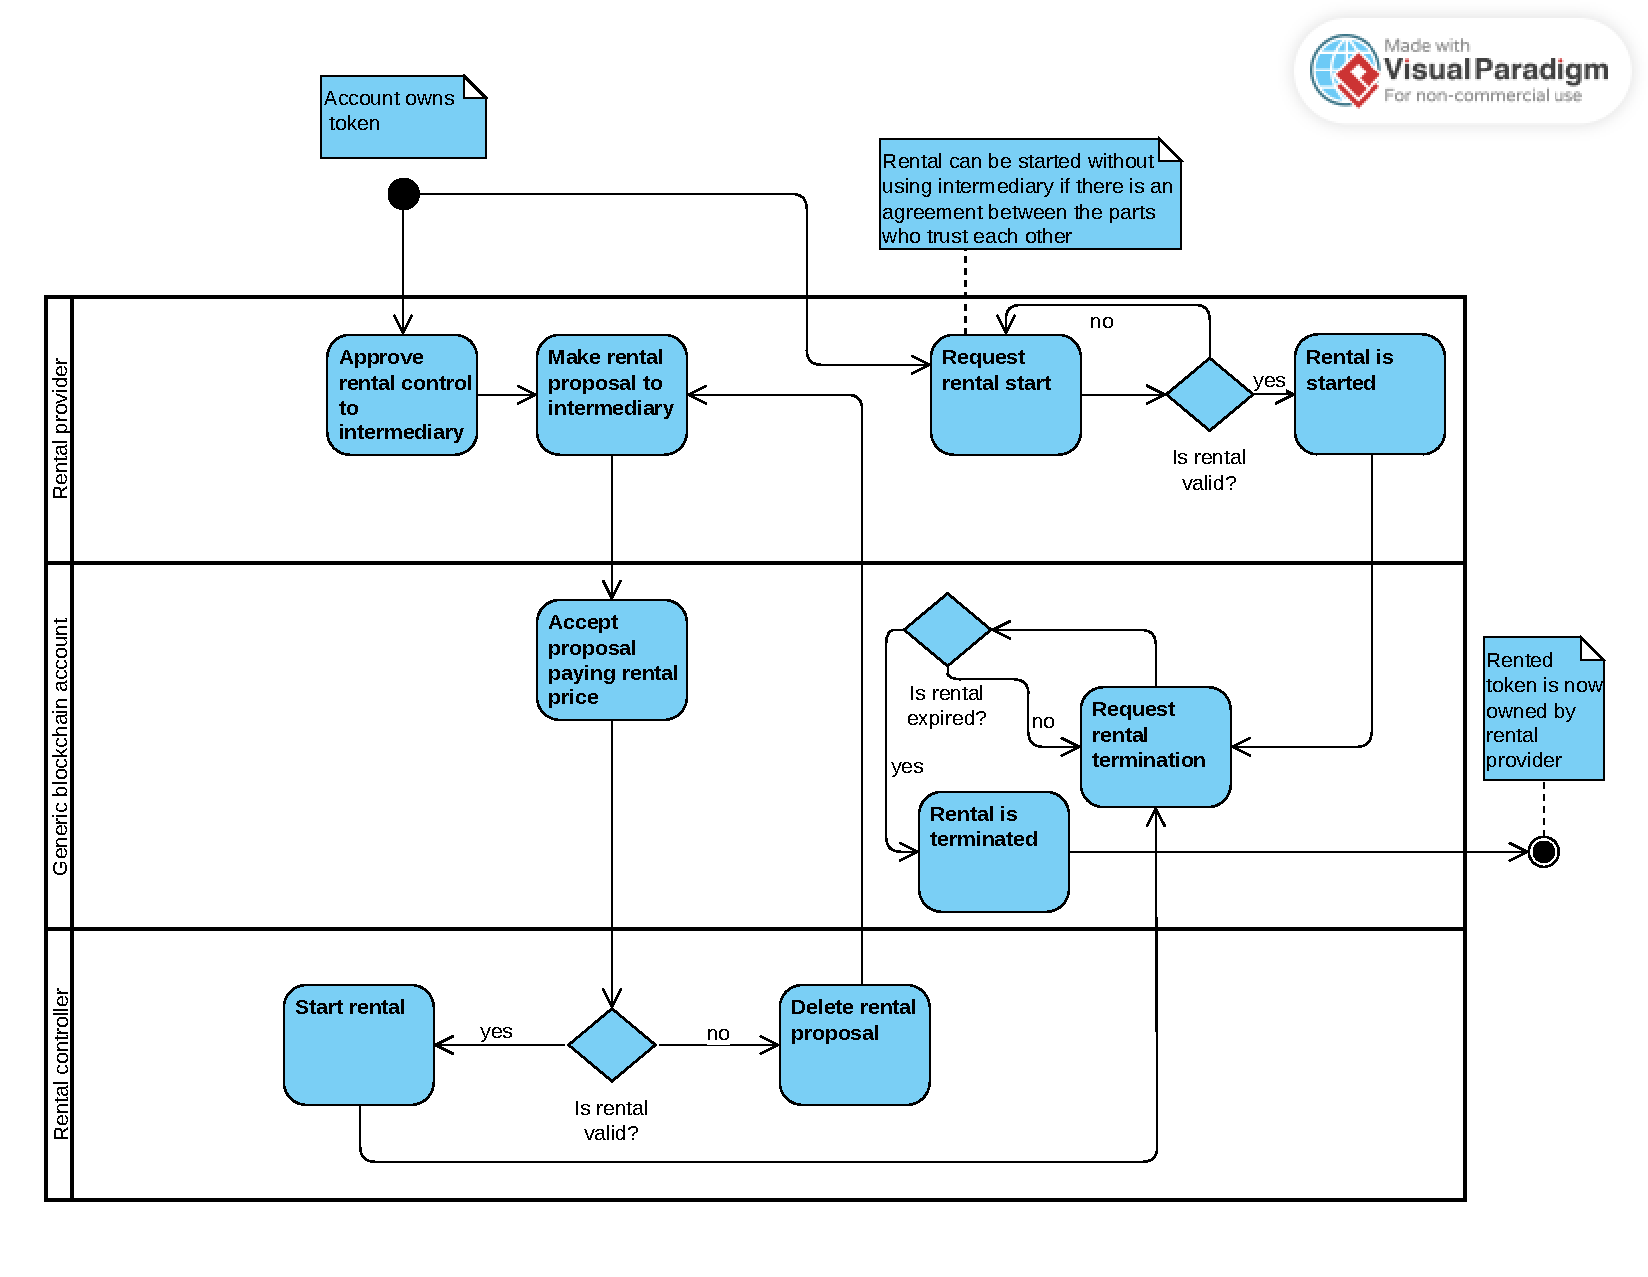
\includegraphics{ActivityDiagrams/activity_rental.pdf} 
        \end{adjustbox}
    \caption{Rental activity diagram}
    \label{fig:Rental AD}
\end{figure}

\subsubsection{Subrental}

Subrental start and termination process, illustrated in Fig.~\ref{fig:Subrental AD} is analogous to the one seen for normal rental. The only meaningful differences are in the initial state, as here the token needs to be rented, and the fact that the decision points also check if subrental is allowed, as it can not be the case.

\begin{figure}[H]
    \centering
        \begin{adjustbox}{width=1\textwidth}
            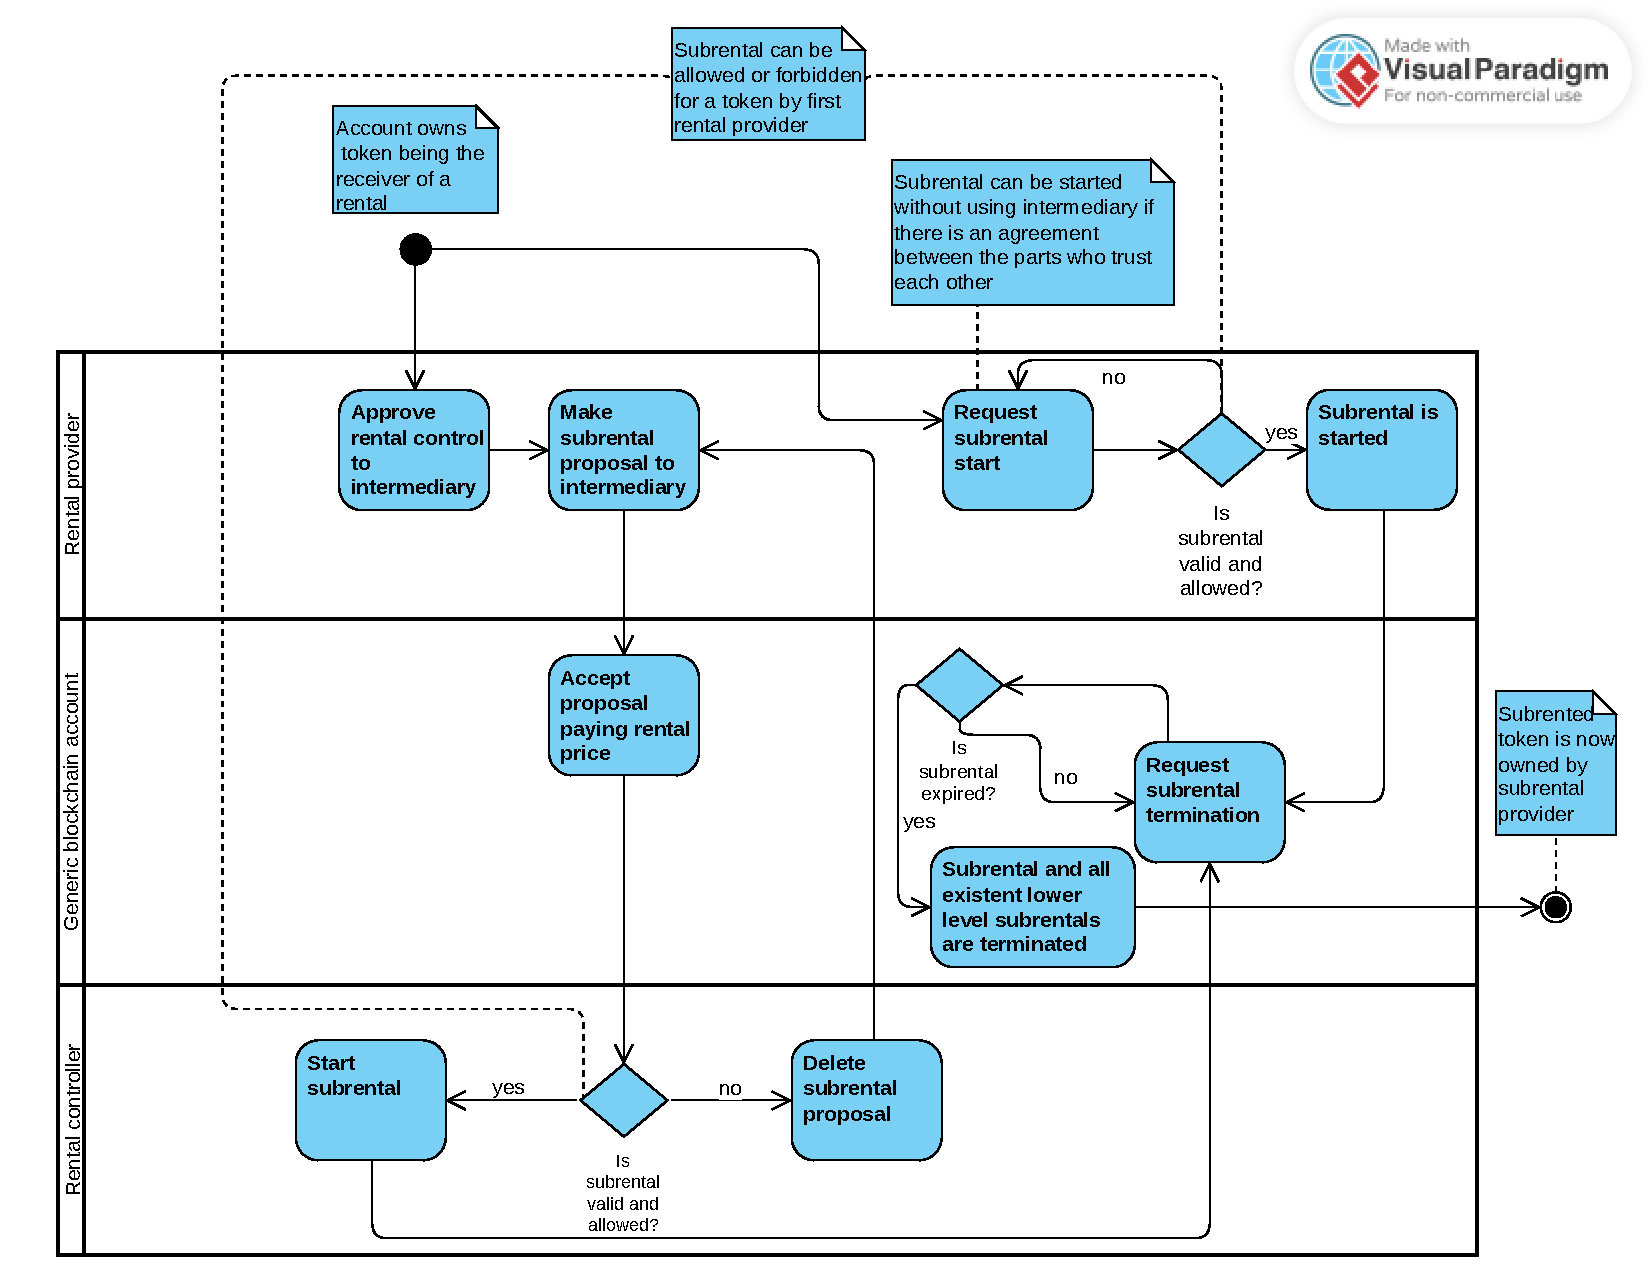
\includegraphics{ActivityDiagrams/activity_subrental.pdf} 
        \end{adjustbox}
    \caption{Subrental activity diagram}
    \label{fig:Subrental AD}
\end{figure}

\subsubsection{Rental period extension}

We can now proceed to rental period extension process. As Fig.~\ref{fig:RentalUpdate AD} depicts, the diagram is quite simple and self-explanatory: it shows how the rental provider can propose an extension to the rental intermediary and the receiver can accept the proposal, making the intermediary update the rental deadline. 

\begin{figure}[H]
    \centering
        \begin{adjustbox}{width=1\textwidth}
            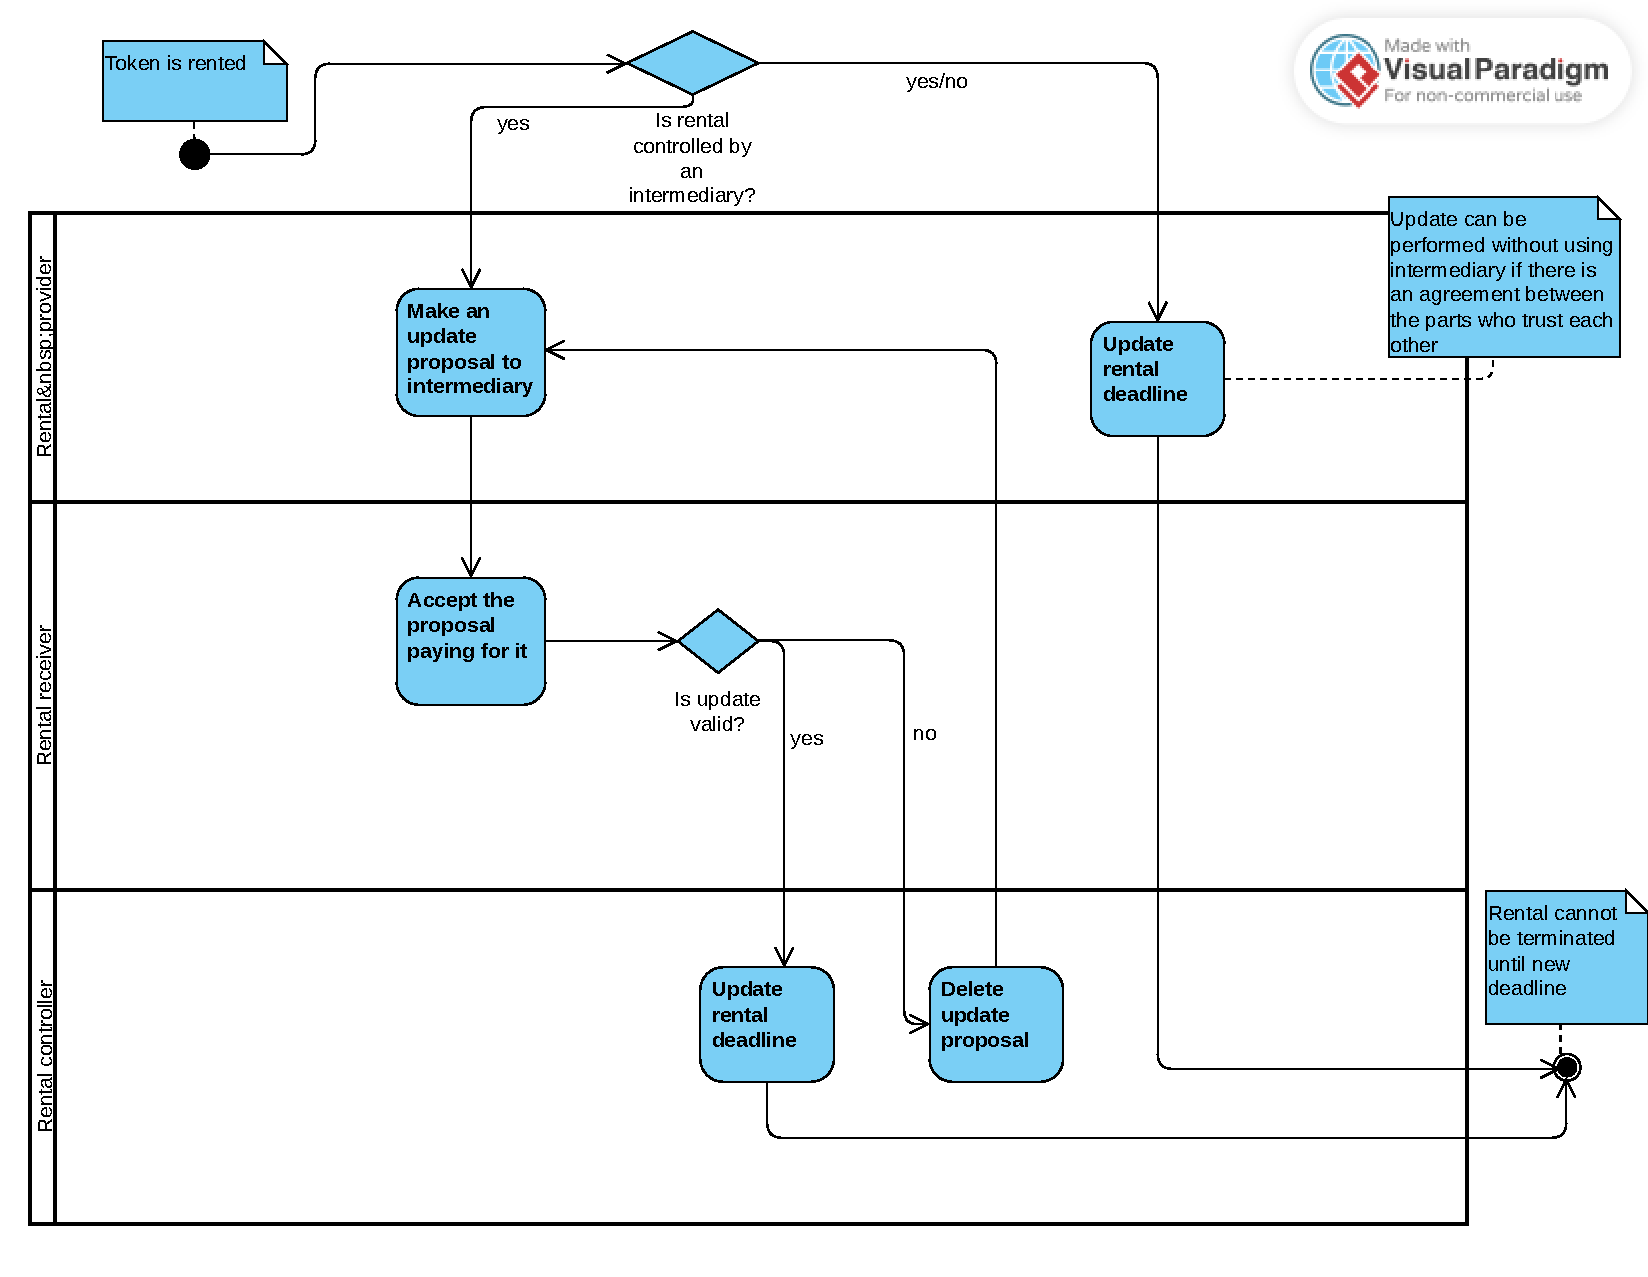
\includegraphics{ActivityDiagrams/activity_rentalUpdate.pdf} 
        \end{adjustbox}
    \caption{Rental period extension activity diagram}
    \label{fig:RentalUpdate AD}
\end{figure}

Again, the usage of the intermediary is optional, hence the rental provider can just directly update the deadline on its own.

\subsubsection{Rented token and rental ownership transfer}

\begin{figure}
    \centering
        \begin{adjustbox}{width=1\textwidth}
            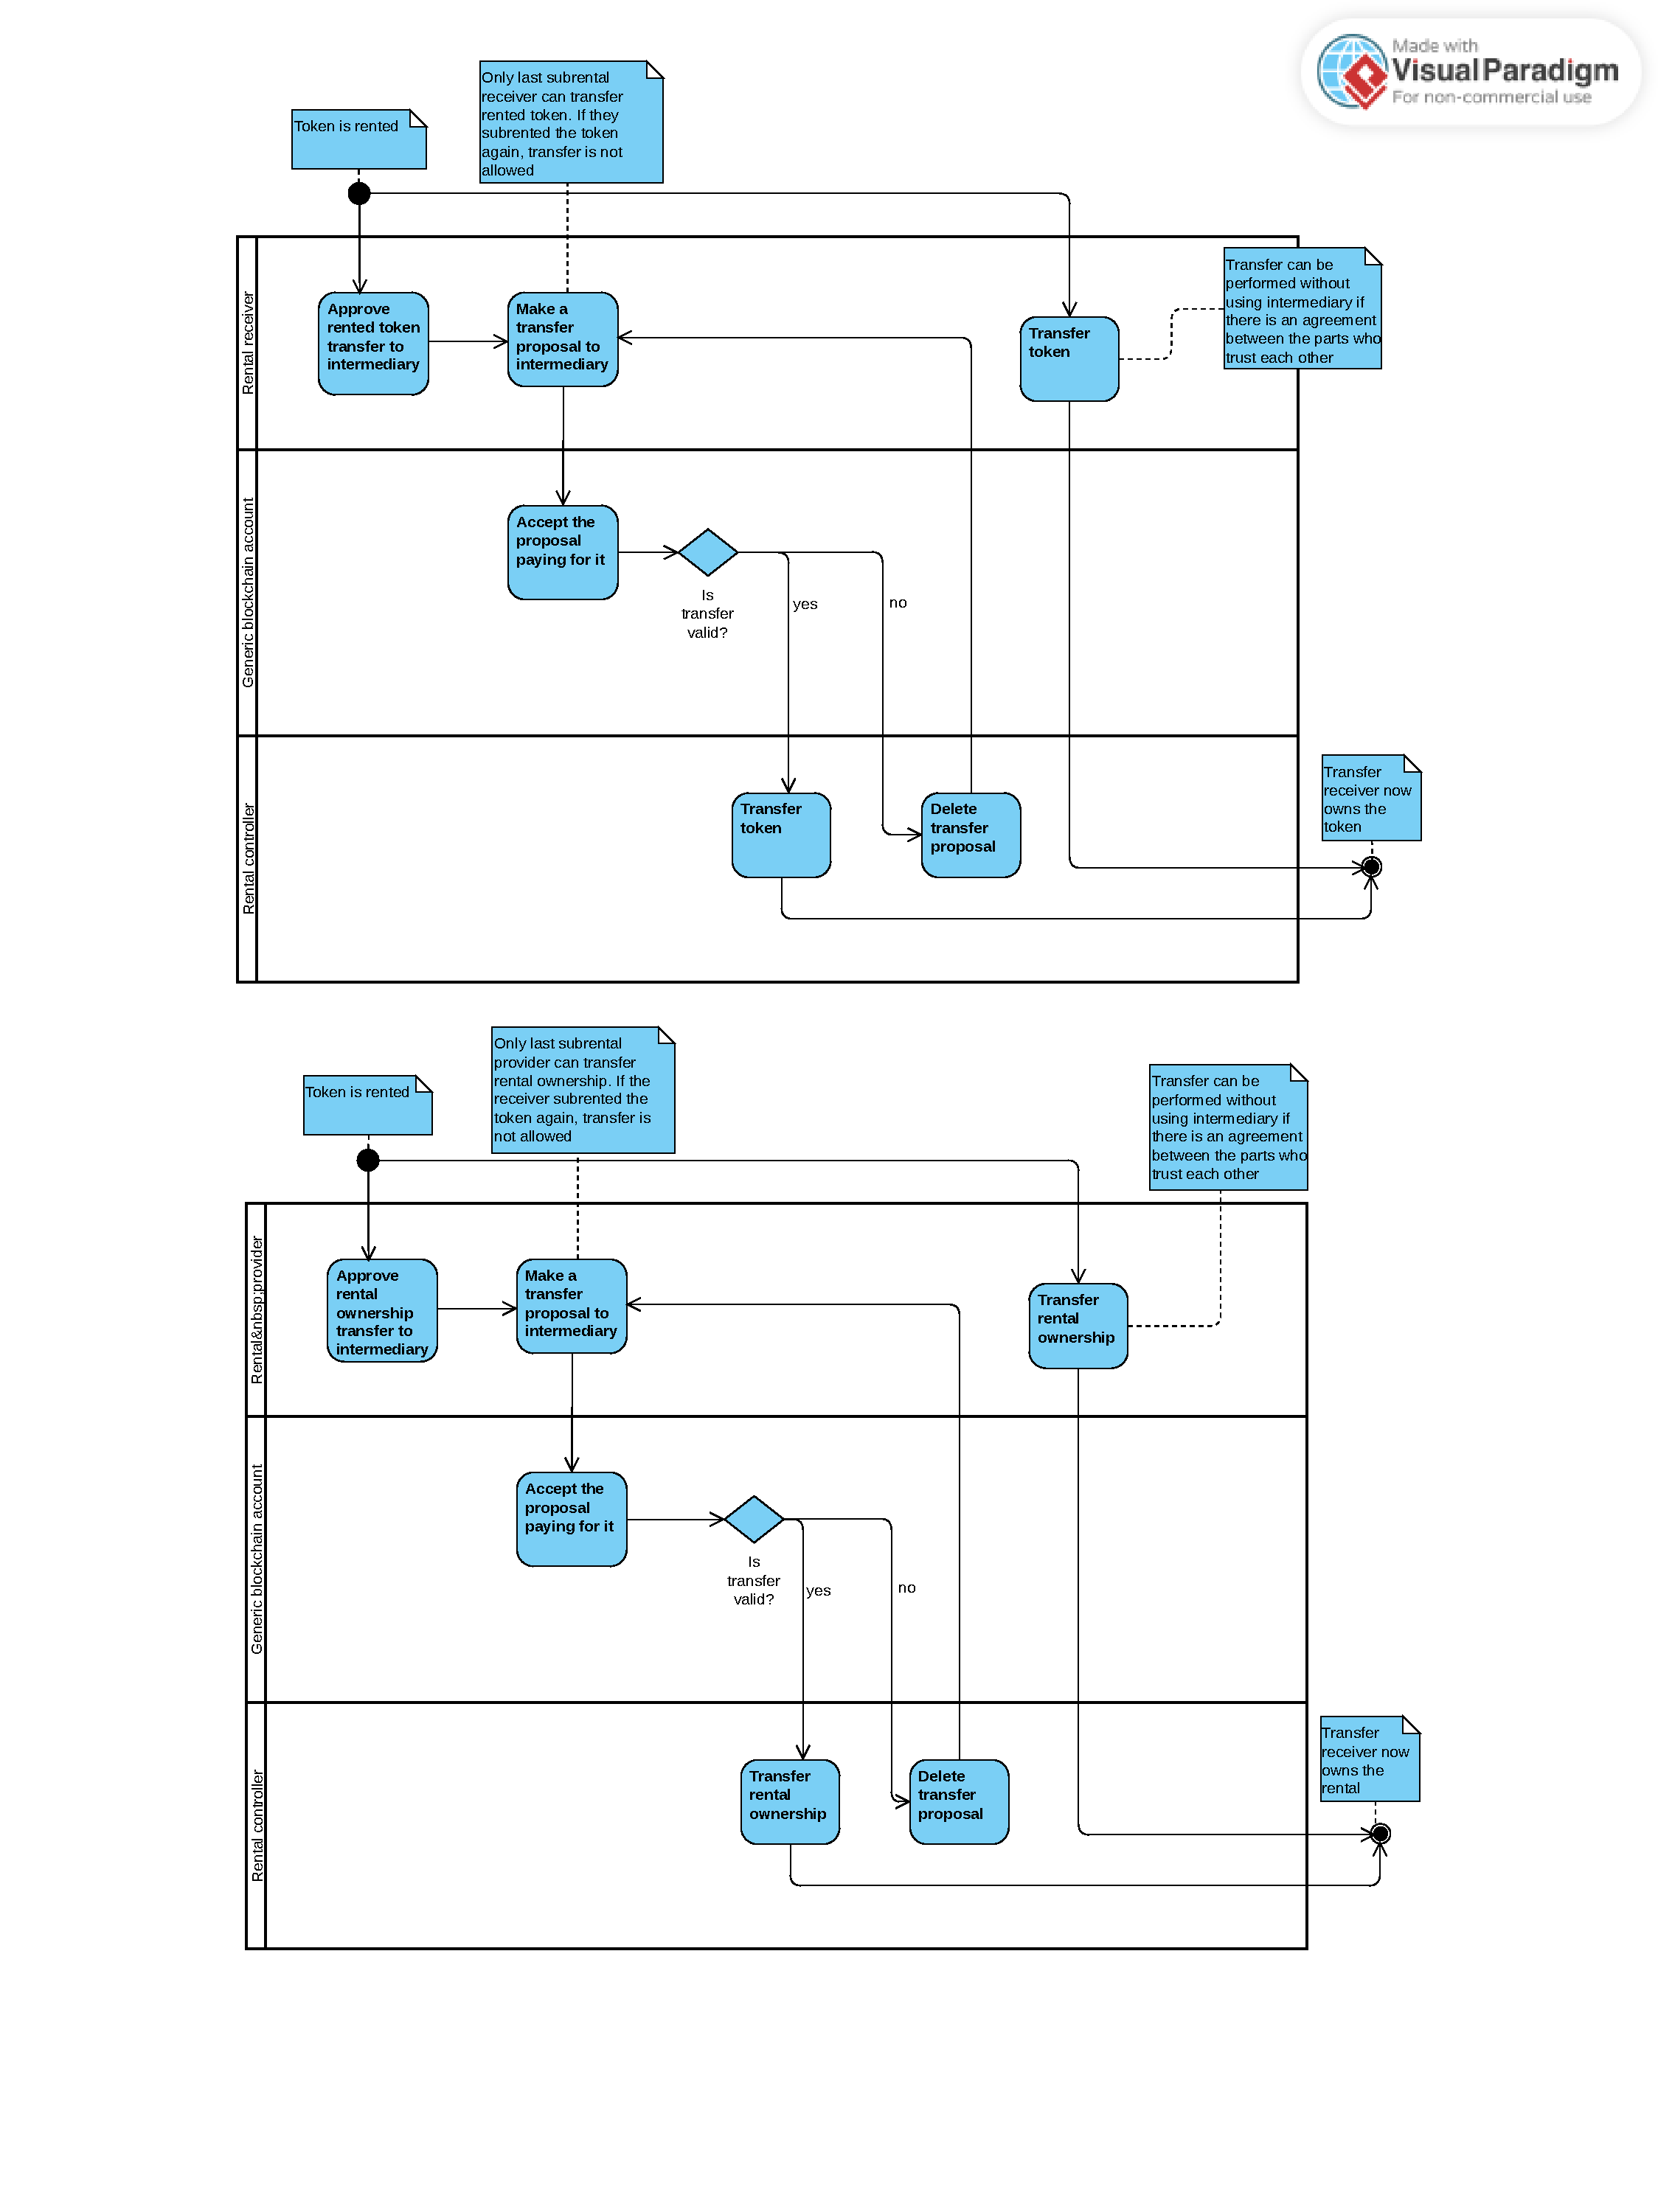
\includegraphics{ActivityDiagrams/activity_rentalTransfer.pdf} 
        \end{adjustbox}
    \caption{Rented token and rental ownership transfer activity diagrams}
    \label{fig:RentalTransfer AD}
\end{figure}

Rented token and rental ownership transfer diagrams are grouped together in Fig.~\ref{fig:RentalTransfer AD} as they depict a very analogous process, with only some of the actors changing between the two. The process is specular to the rental period extension process, with the involved actors having to respectively make a proposal to the intermediary and accept it, after which the intermediary will perform the transfer.
Even these operations can potentially be performed without using an intermediary.

\subsubsection{Rented token redemption}

\begin{figure}[H]
    \centering
        \begin{adjustbox}{width=1\textwidth}
            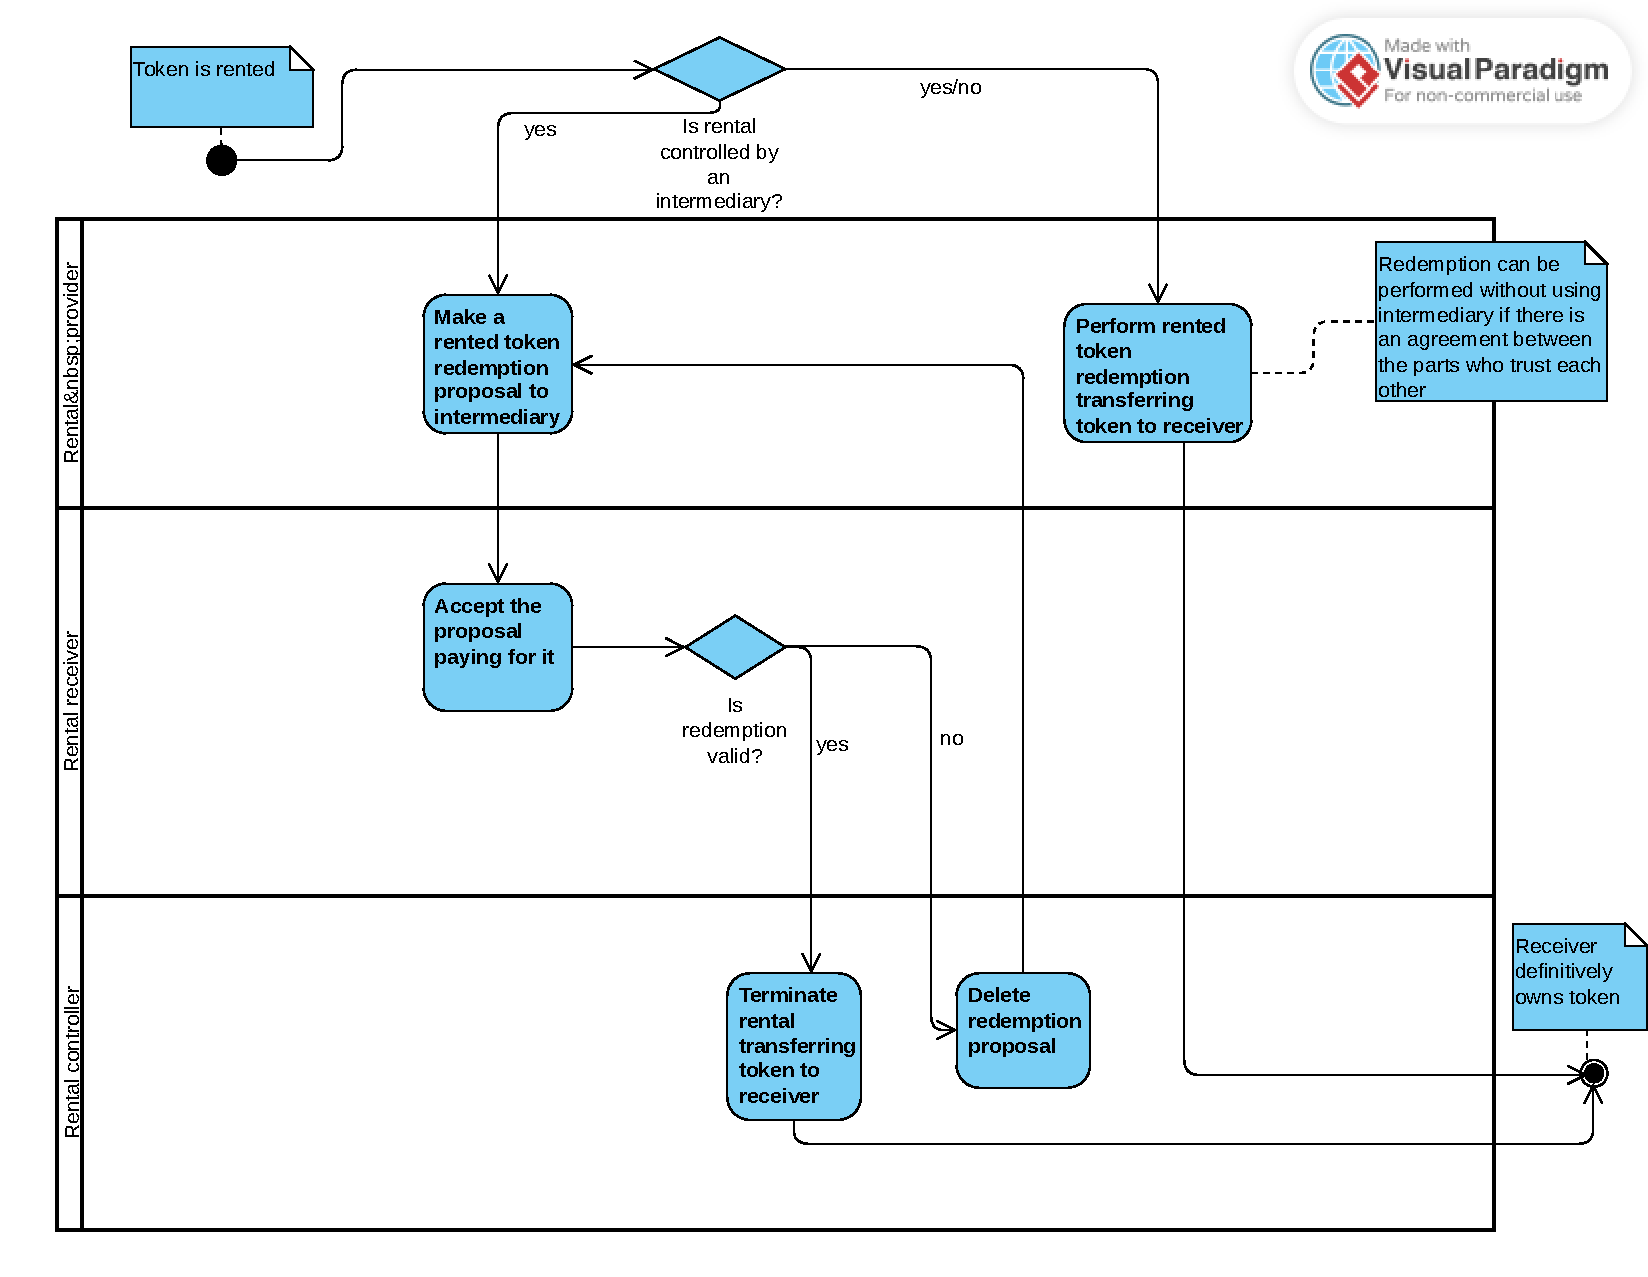
\includegraphics{ActivityDiagrams/activity_rentedTokenRedemption.pdf} 
        \end{adjustbox}
    \caption{Rented token redemption activity diagram}
    \label{fig:RentedTokenRedemption AD}
\end{figure}

This diagram, illustrated in Fig.~\ref{fig:RentedTokenRedemption AD} shows how the receiver of a rental can definitively redeem the rented token. Once again, the diagram is self-explanatory and has no meaningful differences with the previous ones.

\subsubsection{Layaway}

In this diagram, shown in Fig.~\ref{fig:Layaway AD}, we can analyze the full lifecycle of a layaway, from start to termination. The first main difference with the rental process is that here the intermediary is mandatory, hence we don't see the double path out of the initial state.

\begin{figure}[H]
    \centering
        \begin{adjustbox}{width=1\textwidth}
            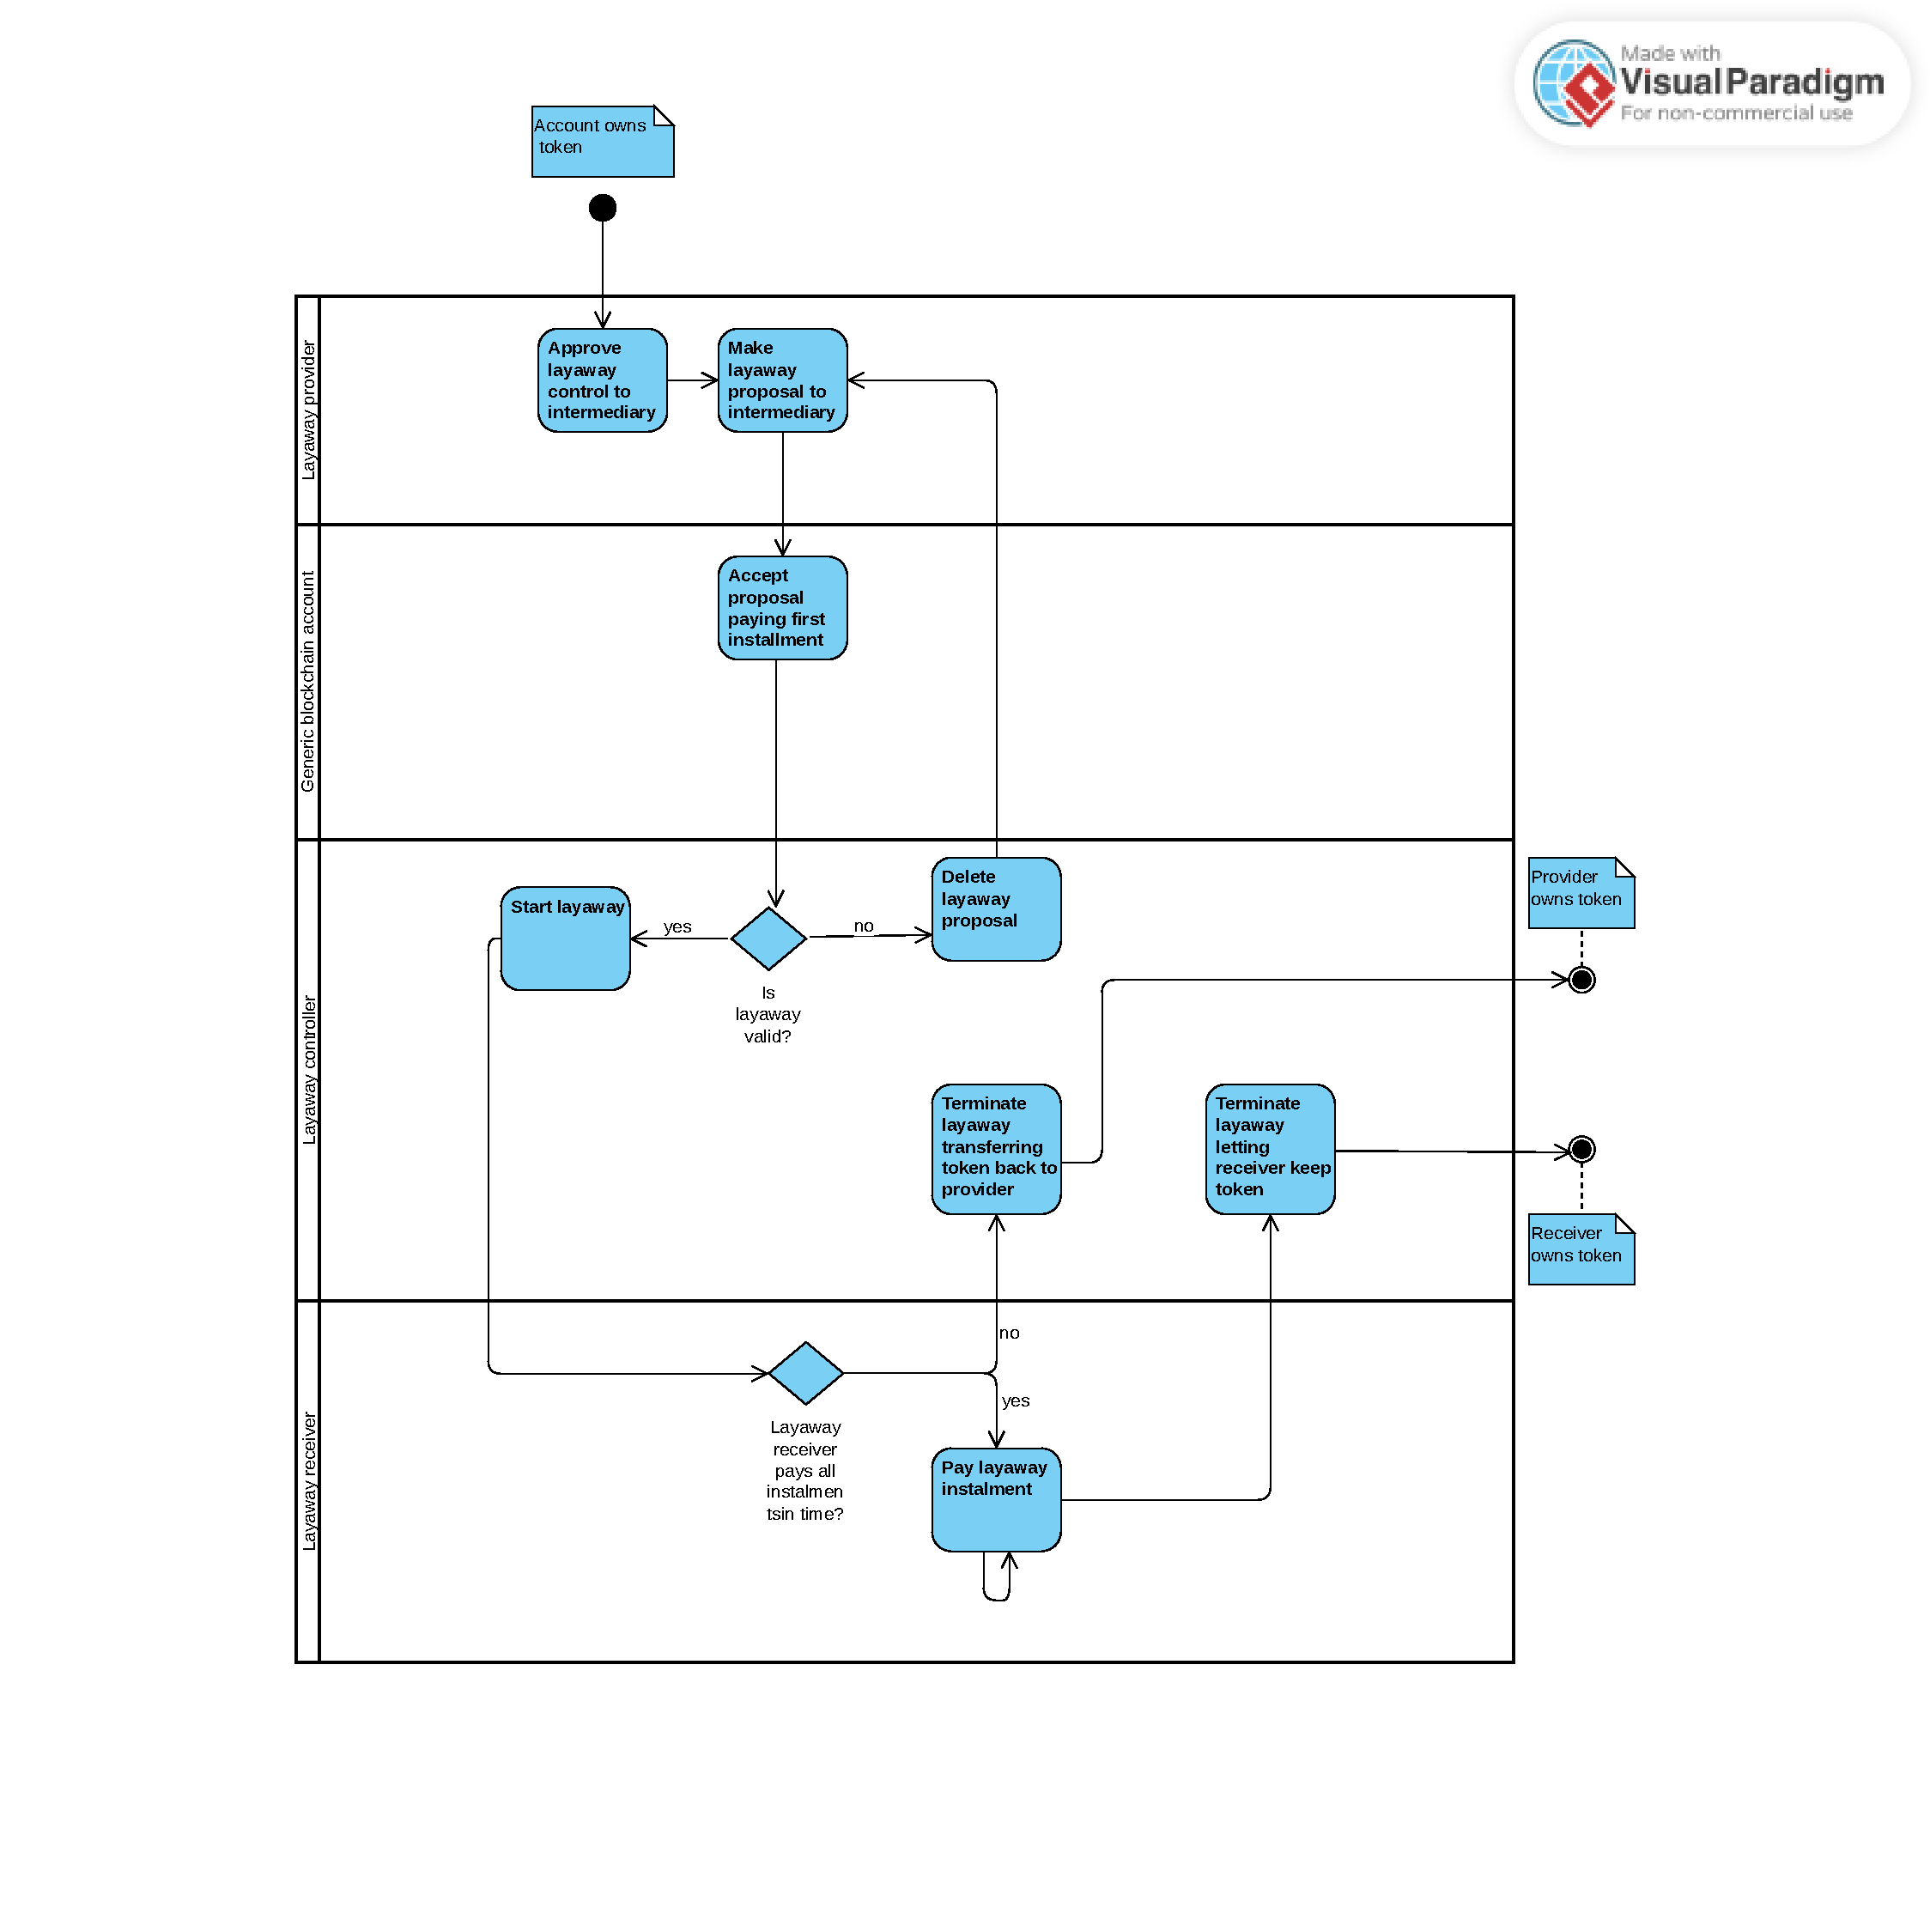
\includegraphics{ActivityDiagrams/activity_layaway.pdf} 
        \end{adjustbox}
    \caption{Layaway activity diagram}
    \label{fig:Layaway AD}
\end{figure}

For what concerns the termination, instead, we see two possible scenarios, which correspond to the correct layaway completion (upon payment of all installments) and the foreclosure of the token (in case of delays on installments payments). This path ramification is the reason why the intermediary is needed, as it will have the responsibility to state if the payments have been completed when the layaway is terminated.

\subsubsection{Layawayed token and layaway ownership transfer}

\begin{figure}[H]
    \centering
        \begin{adjustbox}{width=1\textwidth}
            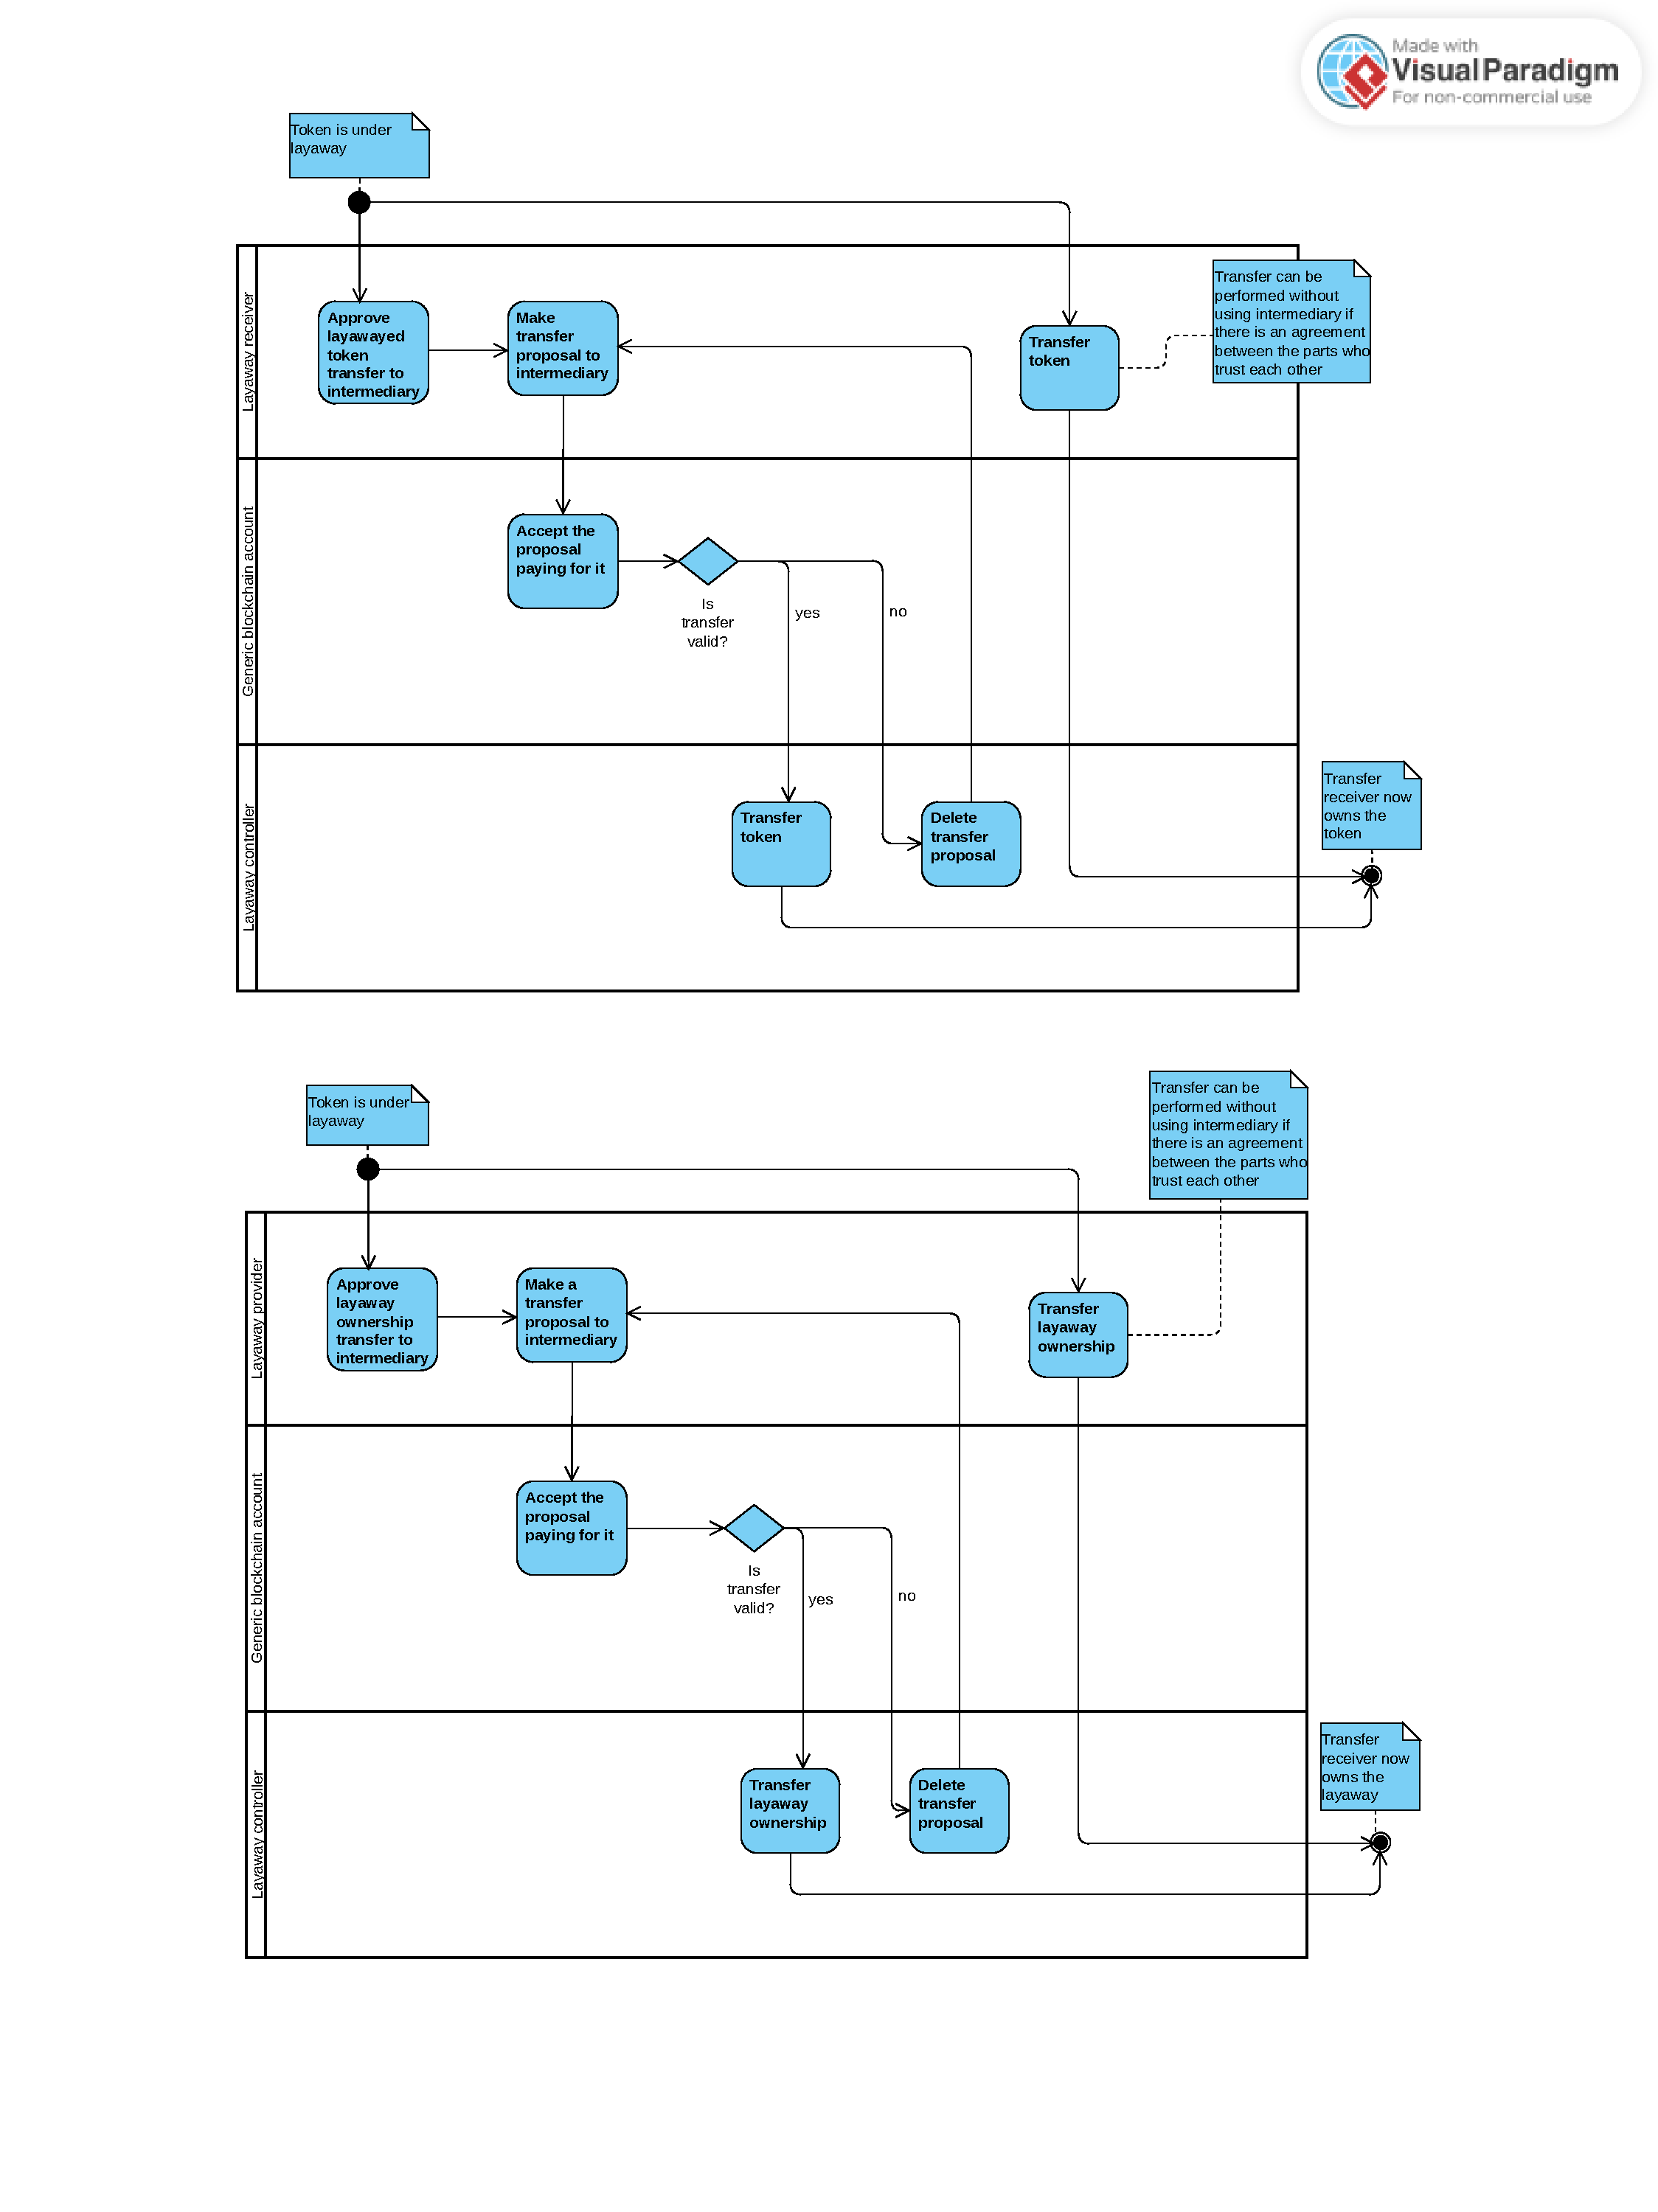
\includegraphics{ActivityDiagrams/activity_layawayTransfer.pdf} 
        \end{adjustbox}
    \caption{Layawayed token and layaway ownership transfer diagrams}
    \label{fig:LayawayTransfer AD}
\end{figure}

Once more, as Fig.~\ref{fig:LayawayTransfer AD} depicts, these diagrams are very similar to the rental ones and aren't worth many comments. They depict the processes of transferring a layawayed token or a layaway ownership. We can however notice how the intermediary is not mandatory for these operations, as it is only needed for layaway termination.


\subsection{Class diagram}

\begin{figure}
    \centering
        \begin{adjustbox}{width=0.9\textwidth}
            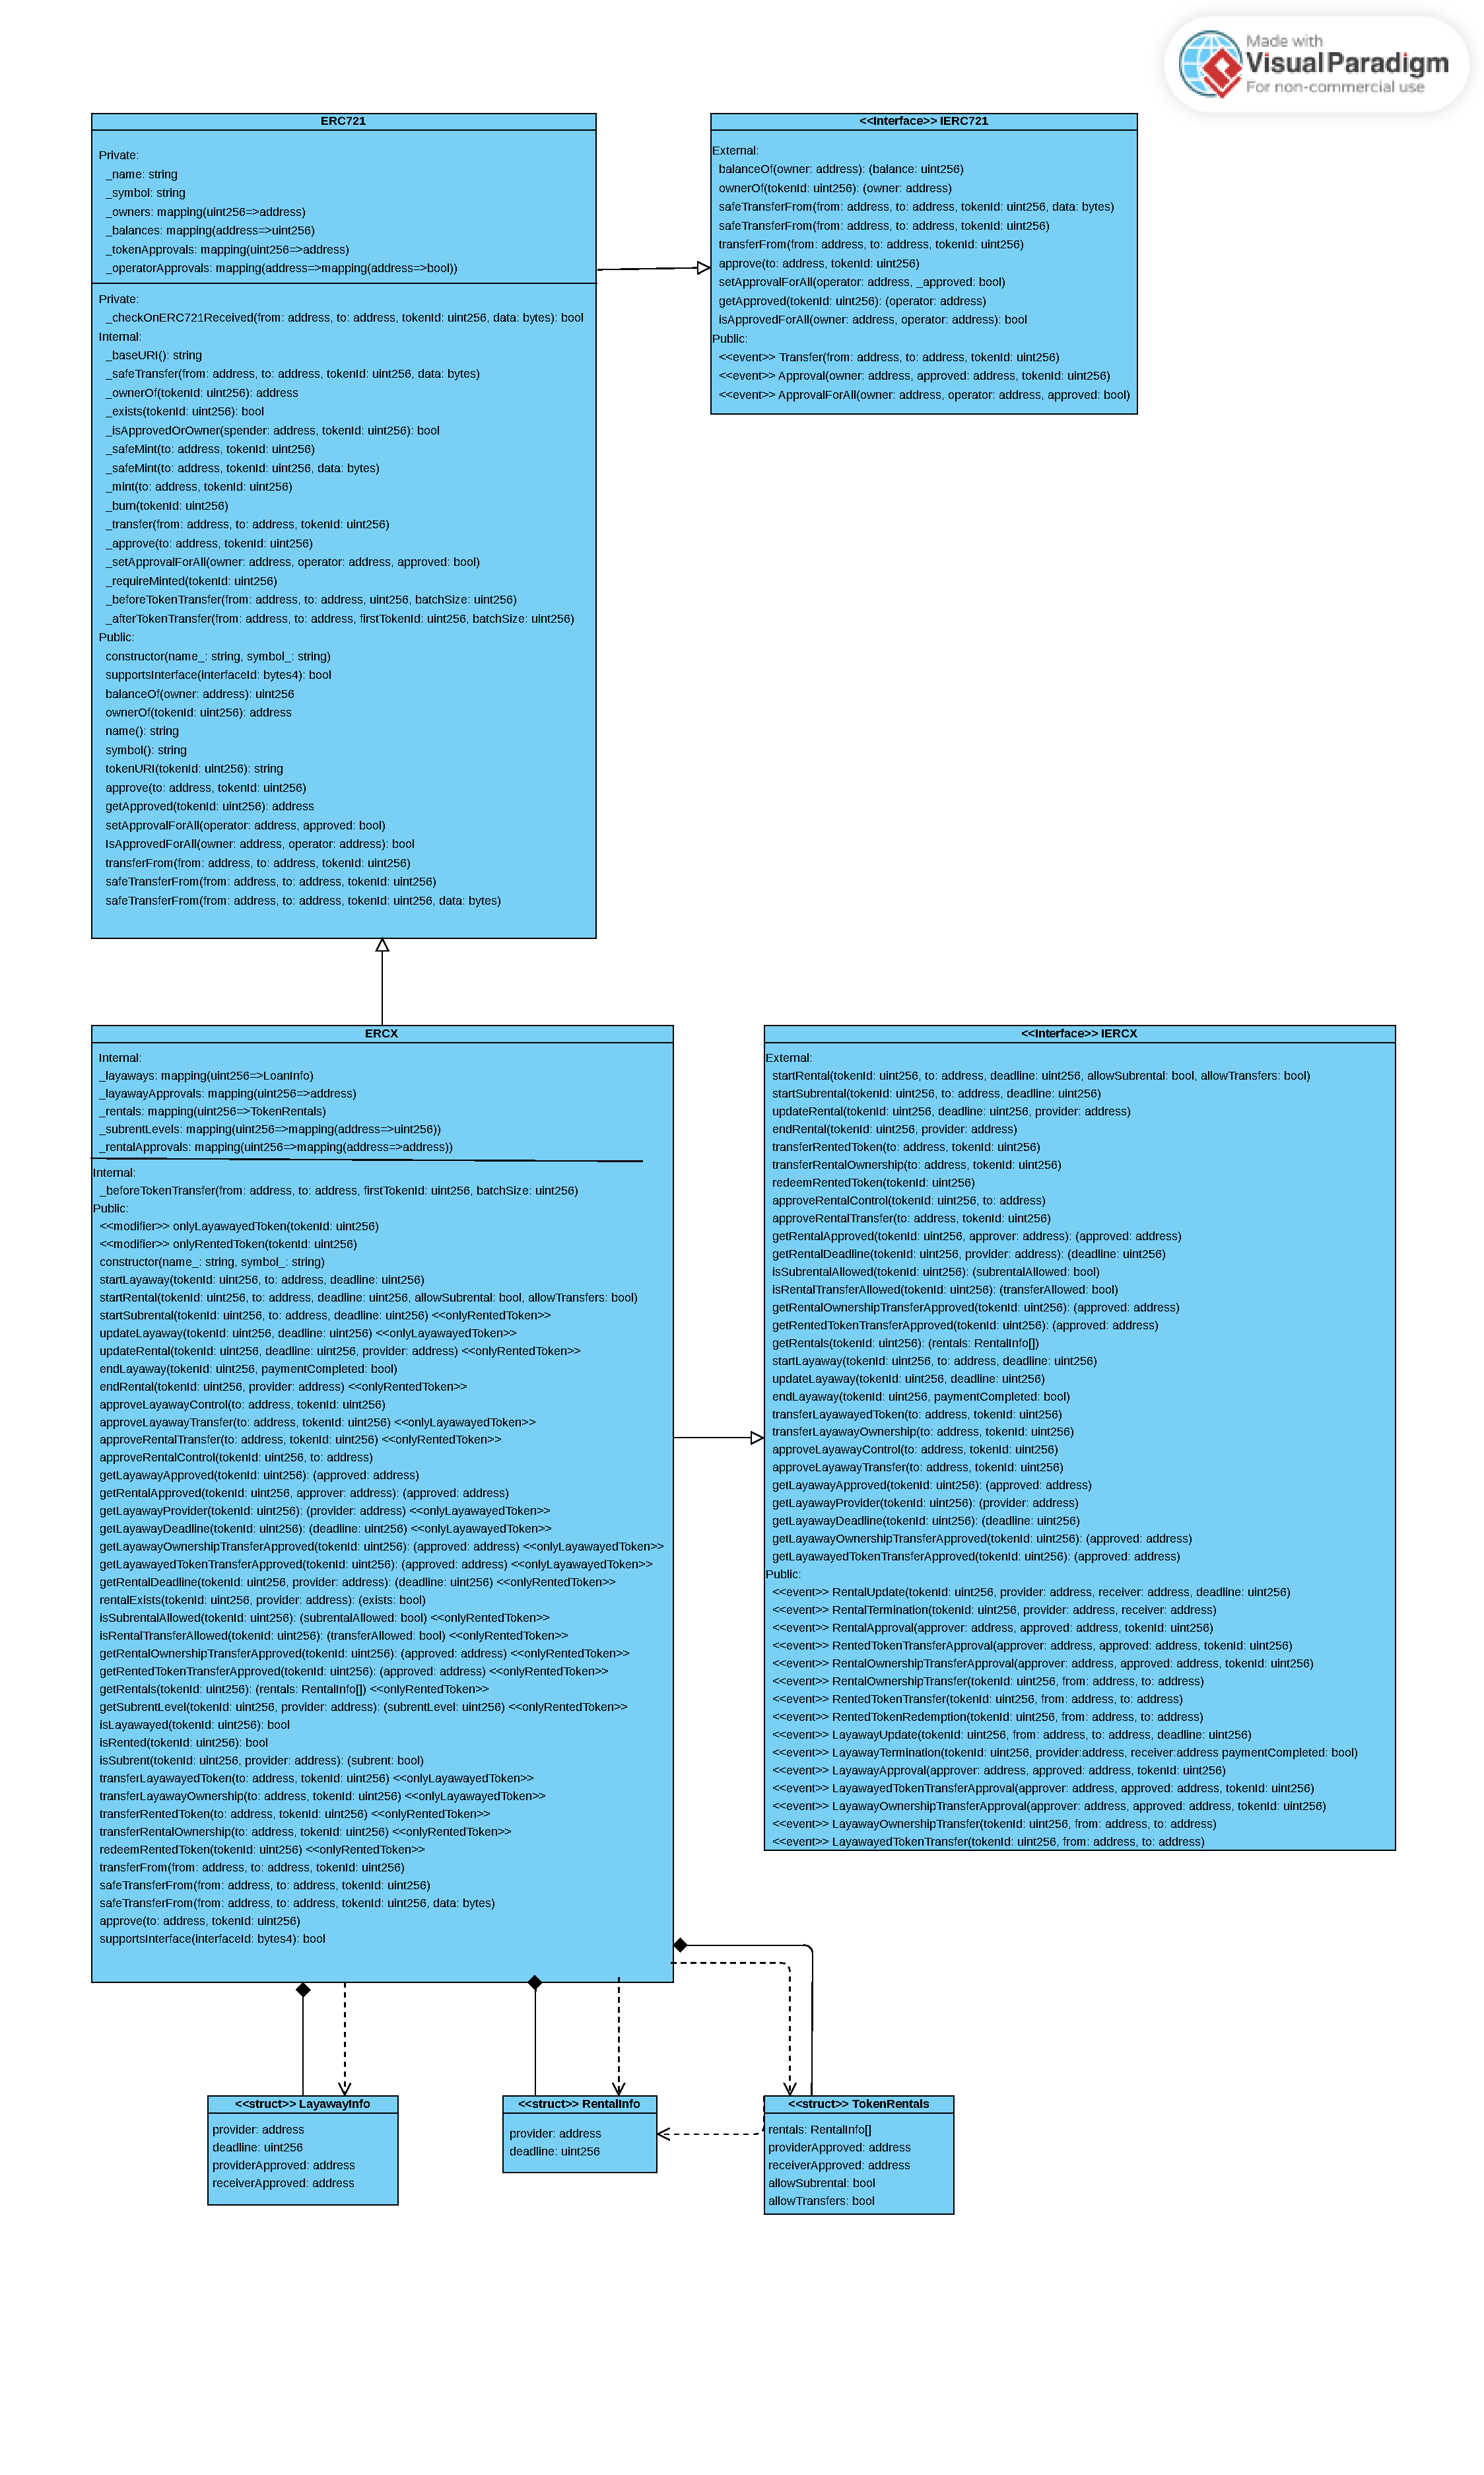
\includegraphics{ClassDiagrams/classDiagram.pdf}
        \end{adjustbox}
    \caption{Class diagram}
    \label{fig:Class diagram}
\end{figure}

Class diagram, illustrated in Fig.~\ref{fig:Class diagram}, is used to show which smart contracts, interfaces and data structures are defined in the proposed solution, and how they are related to each other. As we can notice from the diagram, ERCX smart contract implements the IERCX interface. This interface is the token standard to which every ERCX token collection has to conform, and the ERCX contract is a reference implementation of how such a collection can be coded. If the ERCX standard will be approved and gain attention, any develeper will be welcome to come up with their own implementation, as long as it conforms to IERCX interface.\newline
As introduced in the previous sections, ERCX tokens are meant to rely upon the features of ERC721 tokens and add some new ones: this is achieved by making ERCX contract extend an ERC721 collection contract. In particular, the ERC721 contract chosen for this architecture is Openzeppelin's\cite{ref:openzeppelin} ERC721 reference implementation. Openzeppelin is a blockchain cybersecurity technology and services company, trusted by a lot of the existing  NFT projects. As expected, their ERC721 contract implements IERC721 interface, which is the approved standard for ERC721 tokens.\newline
Other than this, we can also see the non-native data structures used by ERCX contract, which are worth noticing as they appear in some of the functions signatures, hence some knowledge of their shape will be needed when using those functions.


\subsection{Sequence diagrams}
The last diagrams left to show are the sequence diagrams. They depict the same processes seen on the activity diagrams, adding information about the exact functions which need to be used to perform each operation, the raised exceptions (denoted with the notation "revert(reason)", which shows that a description of the reason is contained in the exception), and the events emitted by ERCX contract. Events are the standard way to communicate with a client off-chain application that something has happened on chain; they often contain some attributes which are needed to specify the happened event. \newline
The actual processes unfoldings have yet been explained in the previous diagrams, hence only the mentioned added information will be commented in this section.

\subsubsection{Rental}

\begin{figure}
    \centering
        \begin{adjustbox}{width=1\textwidth}
            \fbox{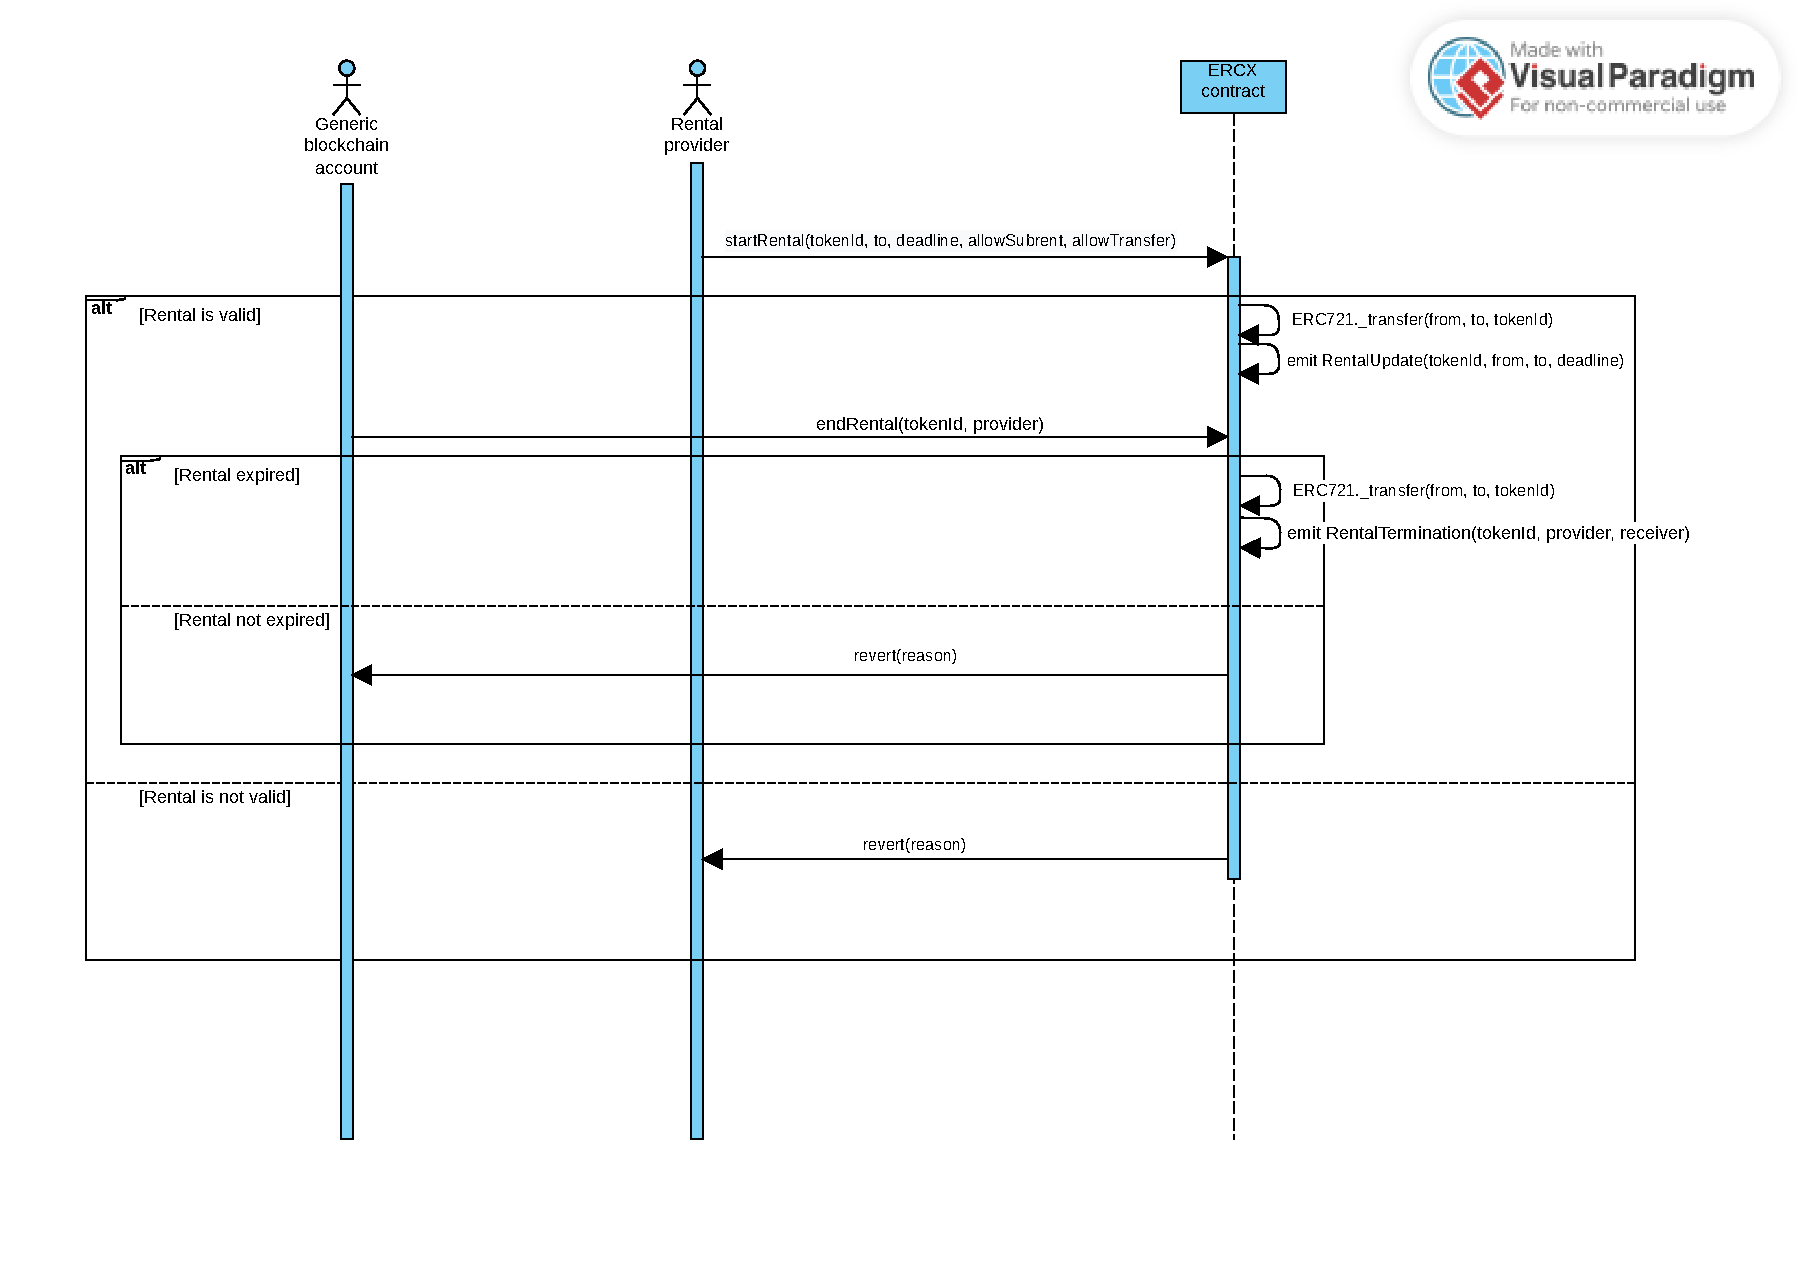
\includegraphics{SequenceDiagrams/sequence_rental.pdf}}
        \end{adjustbox}
    \caption{Rental sequence diagram (without intermediary)}
    \label{fig:Rental SD}
\end{figure}

As Fig.~\ref{fig:Rental SD} shows, this first sequence diagram illustrates the process of renting a NFT without using an intermediary. As we see, the startRental function requires the rental provider to specify the rental duration (using deadline parameter) and to allow or forbid successive subrentals or transfers during rental. With transfers during rental we mean both the rented token transfer and the rental ownership transfer operations.\newline When rental is started, the rented token is transfered to the rental receiver, using ERC721 internal \_transfer function; the event emitted upon rental start is the RentalUpdate event, whose arguments are self-explanatory.\newline
After the rental is started, any account is able to call the endRental function: this function only has to check that the rental deadline is expired and subsequently end the rental, returning the rented token to the provider; there is no need to restrict the allowed callers to some specific actors. At this point, a RentalTermination event is emitted.


\begin{figure}
    \centering
        \begin{adjustbox}{width=1\textwidth}
            \fbox{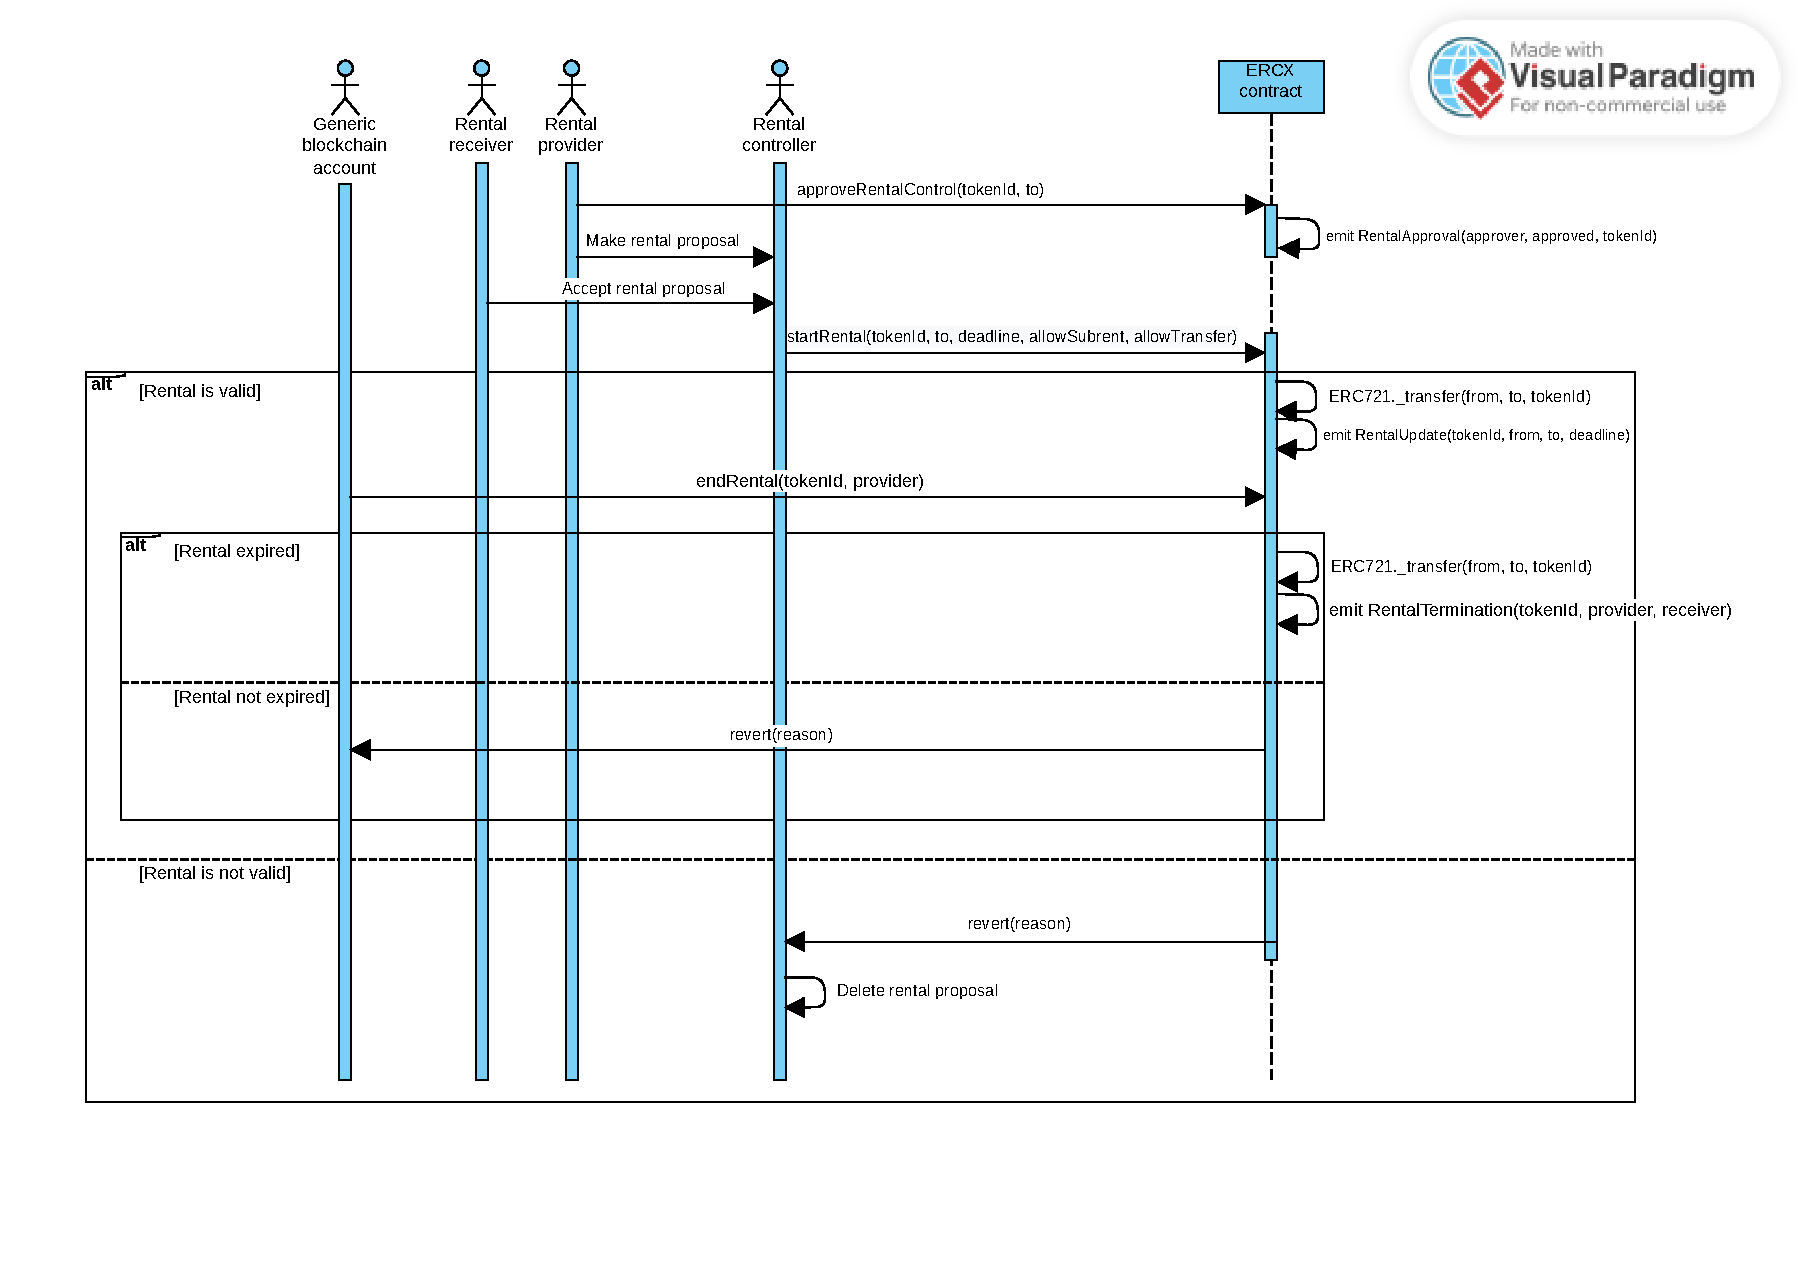
\includegraphics{SequenceDiagrams/sequence_rental_intermediary.pdf}}
        \end{adjustbox}
    \caption{Rental sequence diagram (with intermediary)}
    \label{fig:Rental_intermediary SD}
\end{figure}

We can now move on to analyze the diagram describing how to start and terminate a rental when an intermediary is used. As Fig.~\ref{fig:Rental_intermediary SD} depicts, the main differences with the previous diagram are at the beginning: here, the rental provider doesn't start the rental on its own; they instead have to use approveRentalControl function to nominate an account (normally a contract) as intermediary. After this, rental provider and receiver can find a rental agreement using the intermediary: when the receiver accepts provider's proposal, the intermediary will start the rental using startRental function, as seen above. After this point, the diagram is identical to the previous one, except for the particular that the intermediary has to delete rental proposals if the proposed rental turns out to be not valid.


\subsubsection{Subrental}

\begin{figure}
    \centering
        \begin{adjustbox}{width=1\textwidth}
            \fbox{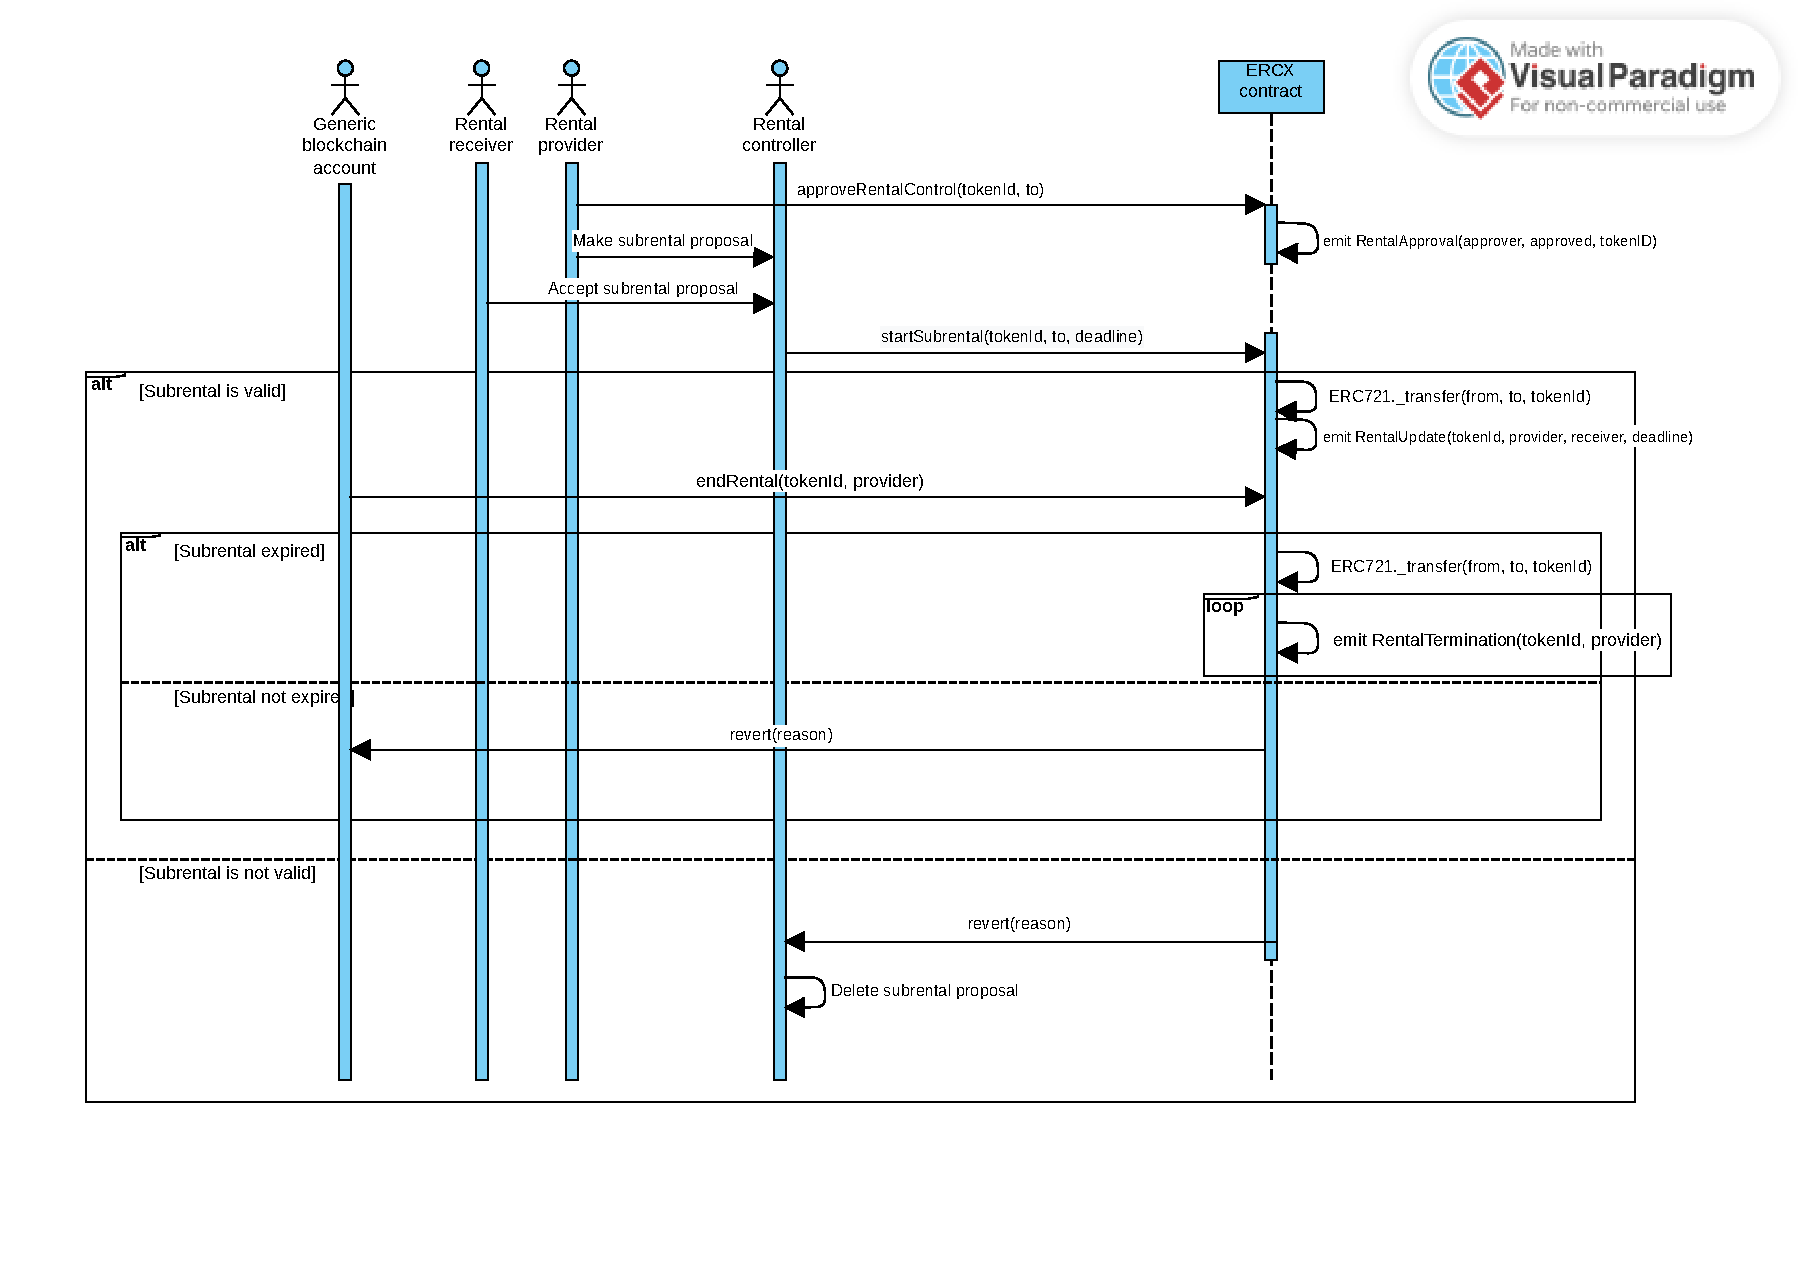
\includegraphics{SequenceDiagrams/sequence_subrental_intermediary.pdf}}
        \end{adjustbox}
    \caption{Subrental sequence diagram}
    \label{fig:Subrental SD}
\end{figure}

Subrental process, illustrated in Fig.~\ref{fig:Subrental SD}, is completely analogous to simple rental, except for the fact that when a subrental is terminated, all the other subsequent lower level subrentals must be terminated, if any. This is why the RentalTermination event appears inside a loop.\newline
\bigskip

\subsubsection{Rental period extension}

\begin{figure}
    \centering
        \begin{adjustbox}{width=1\textwidth}
            \fbox{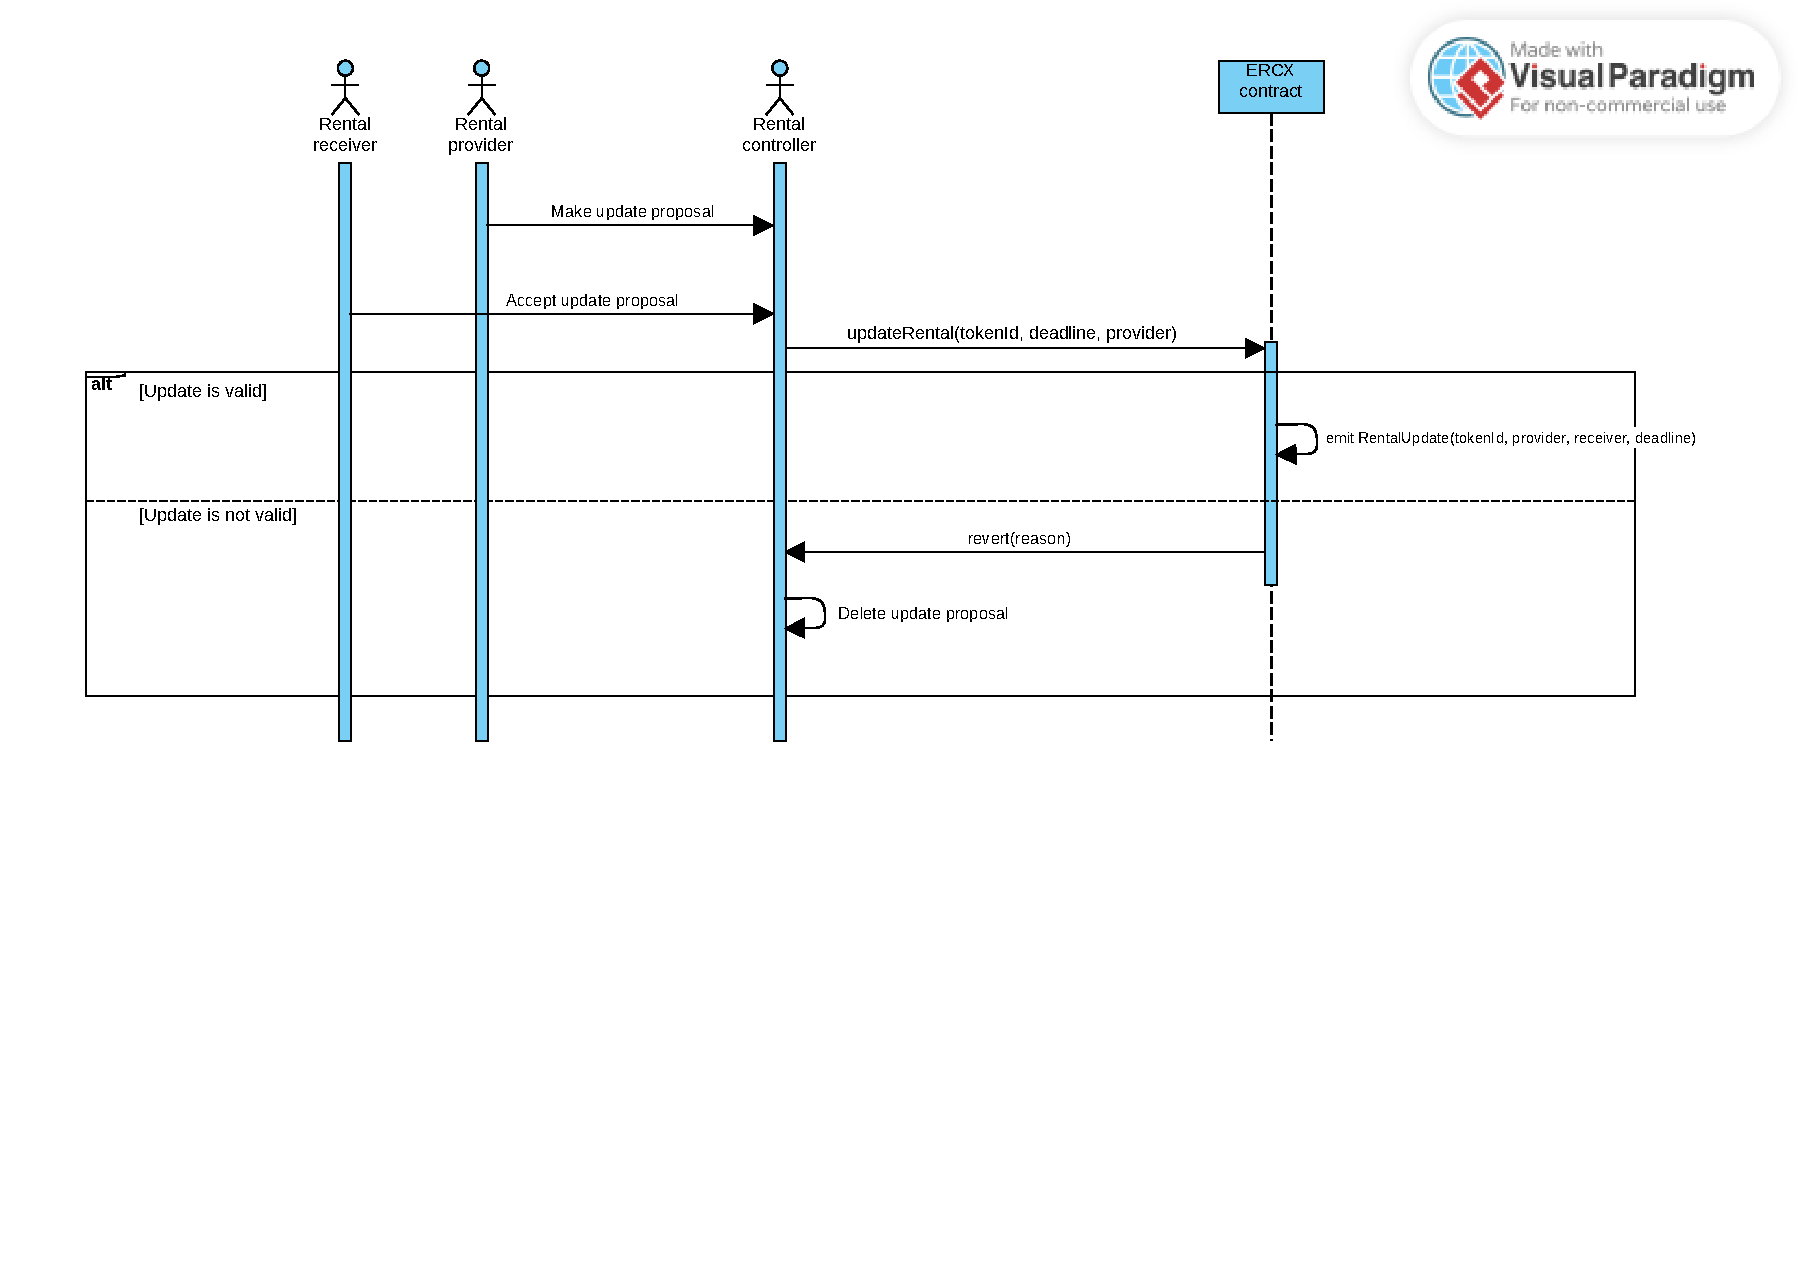
\includegraphics{SequenceDiagrams/sequence_rentalUpdate.pdf}}
        \end{adjustbox}
    \caption{Rental period extension sequence diagram}
    \label{fig:RentalUpdate SD}
\end{figure}

Next diagram we want to analyze is the one describing rental period extension procedure, shown in Fig.~\ref{fig:RentalUpdate SD}. From now on, we will only show the versions of the diagrams using the intermediary, as this will be the mainly used solution, and moreover the diagrams without the intermediary would be quite similar and repetitive. We have shown the difference between using an intermediary and not using it in the first two rental diagrams, and it would be analogous for all the other functionalities.\newline
Similarly to the previous diagrams, we have the rental provider making a proposal to the intermediary, and the receiver accepting it. Once this is done, the intermediary delays the rental deadline using UpdateRental function and causing the emission of a RentalUpdate event (the same emitted on rental start).\newline
\bigskip

\subsubsection{Rented token transfer}

\begin{figure}
    \centering
        \begin{adjustbox}{width=1\textwidth}
            \fbox{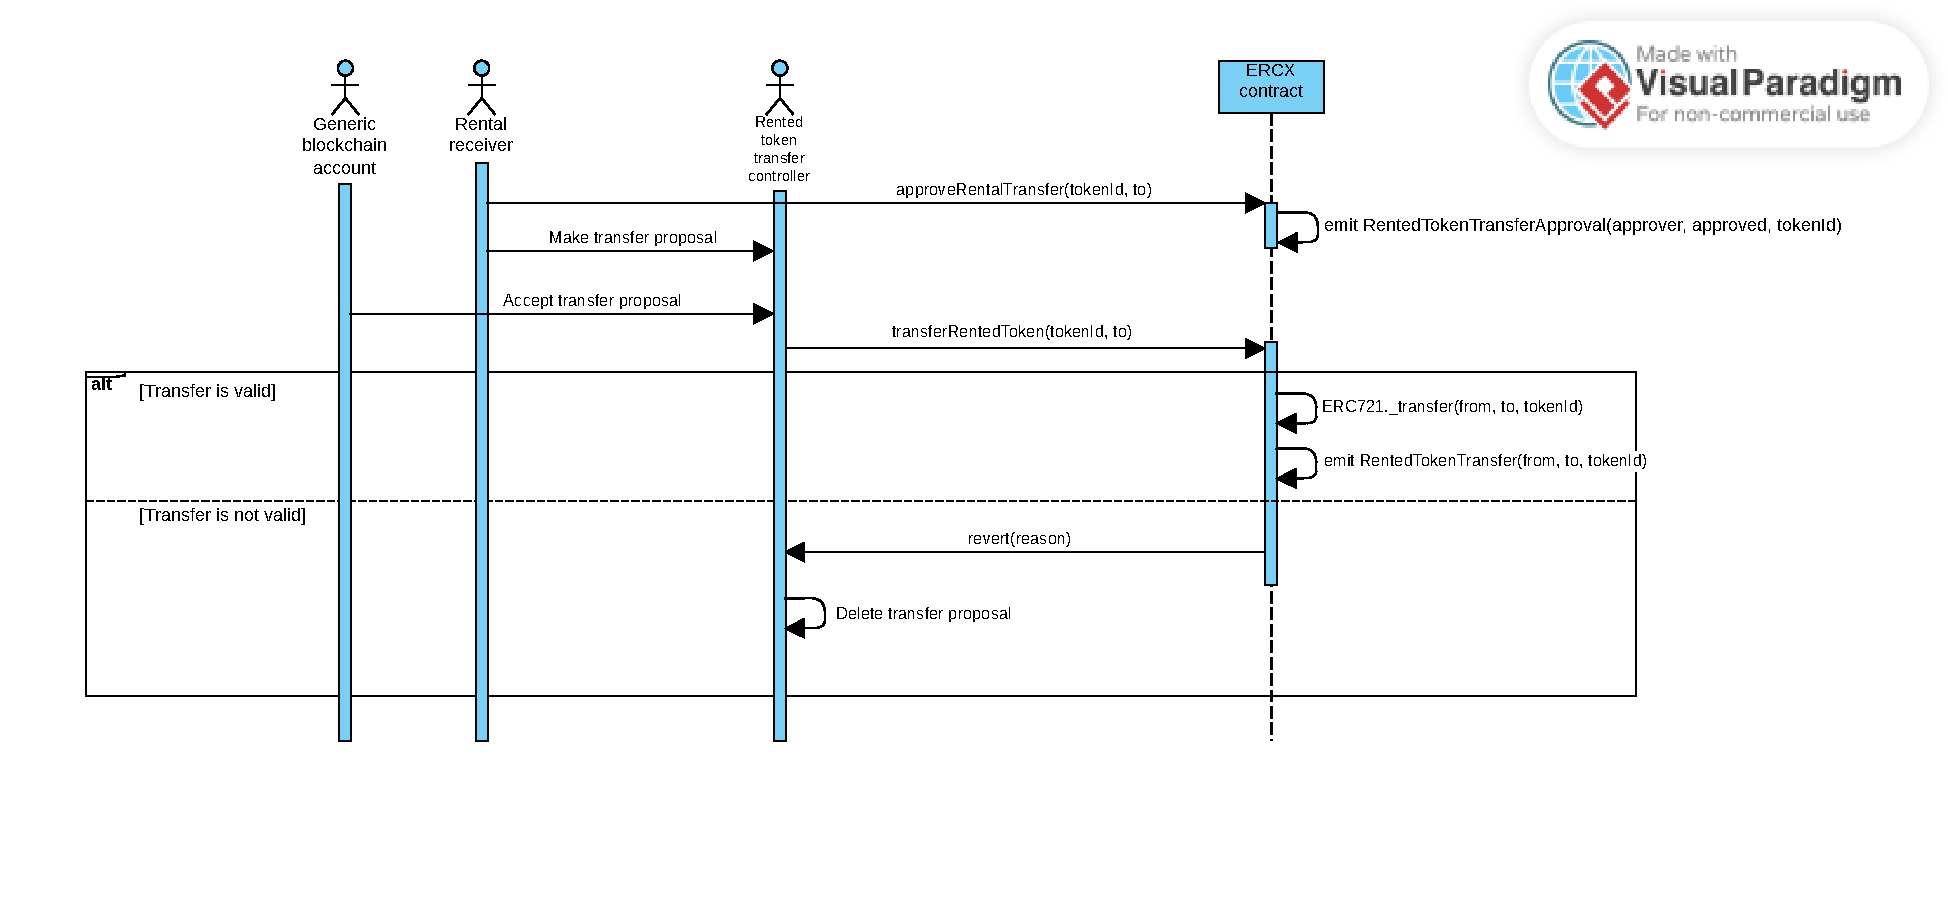
\includegraphics{SequenceDiagrams/sequence_rentedTokenTransfer.pdf}}
        \end{adjustbox}
    \caption{Rented token transfer sequence diagram}
    \label{fig:RentedTokenTransfer SD}
\end{figure}

In Fig.~\ref{fig:RentedTokenTransfer SD}, we illustrate the process of a rental receiver transferring a rented token to a new receiver. We can first of all notice how rented token transfer controller actor is different from the normal rental controller: this means that the two intermediaries do not necessarily need to be the same account; the function used to nominate a rented token transfer intermediary is the approveRentalTransfer function. After transfer control has been approved, rental receiver can find an agreement on transfer price with an account interested in the rented NFT; at this point, the approved intermediary will use transferRentedToken function to perform the agreed transfer. This causes ERCX contract to emit a RentedTokenTransfer event.\newline
\bigskip

\subsubsection{Rental ownership transfer}

\begin{figure}
    \centering
        \begin{adjustbox}{width=1\textwidth}
            \fbox{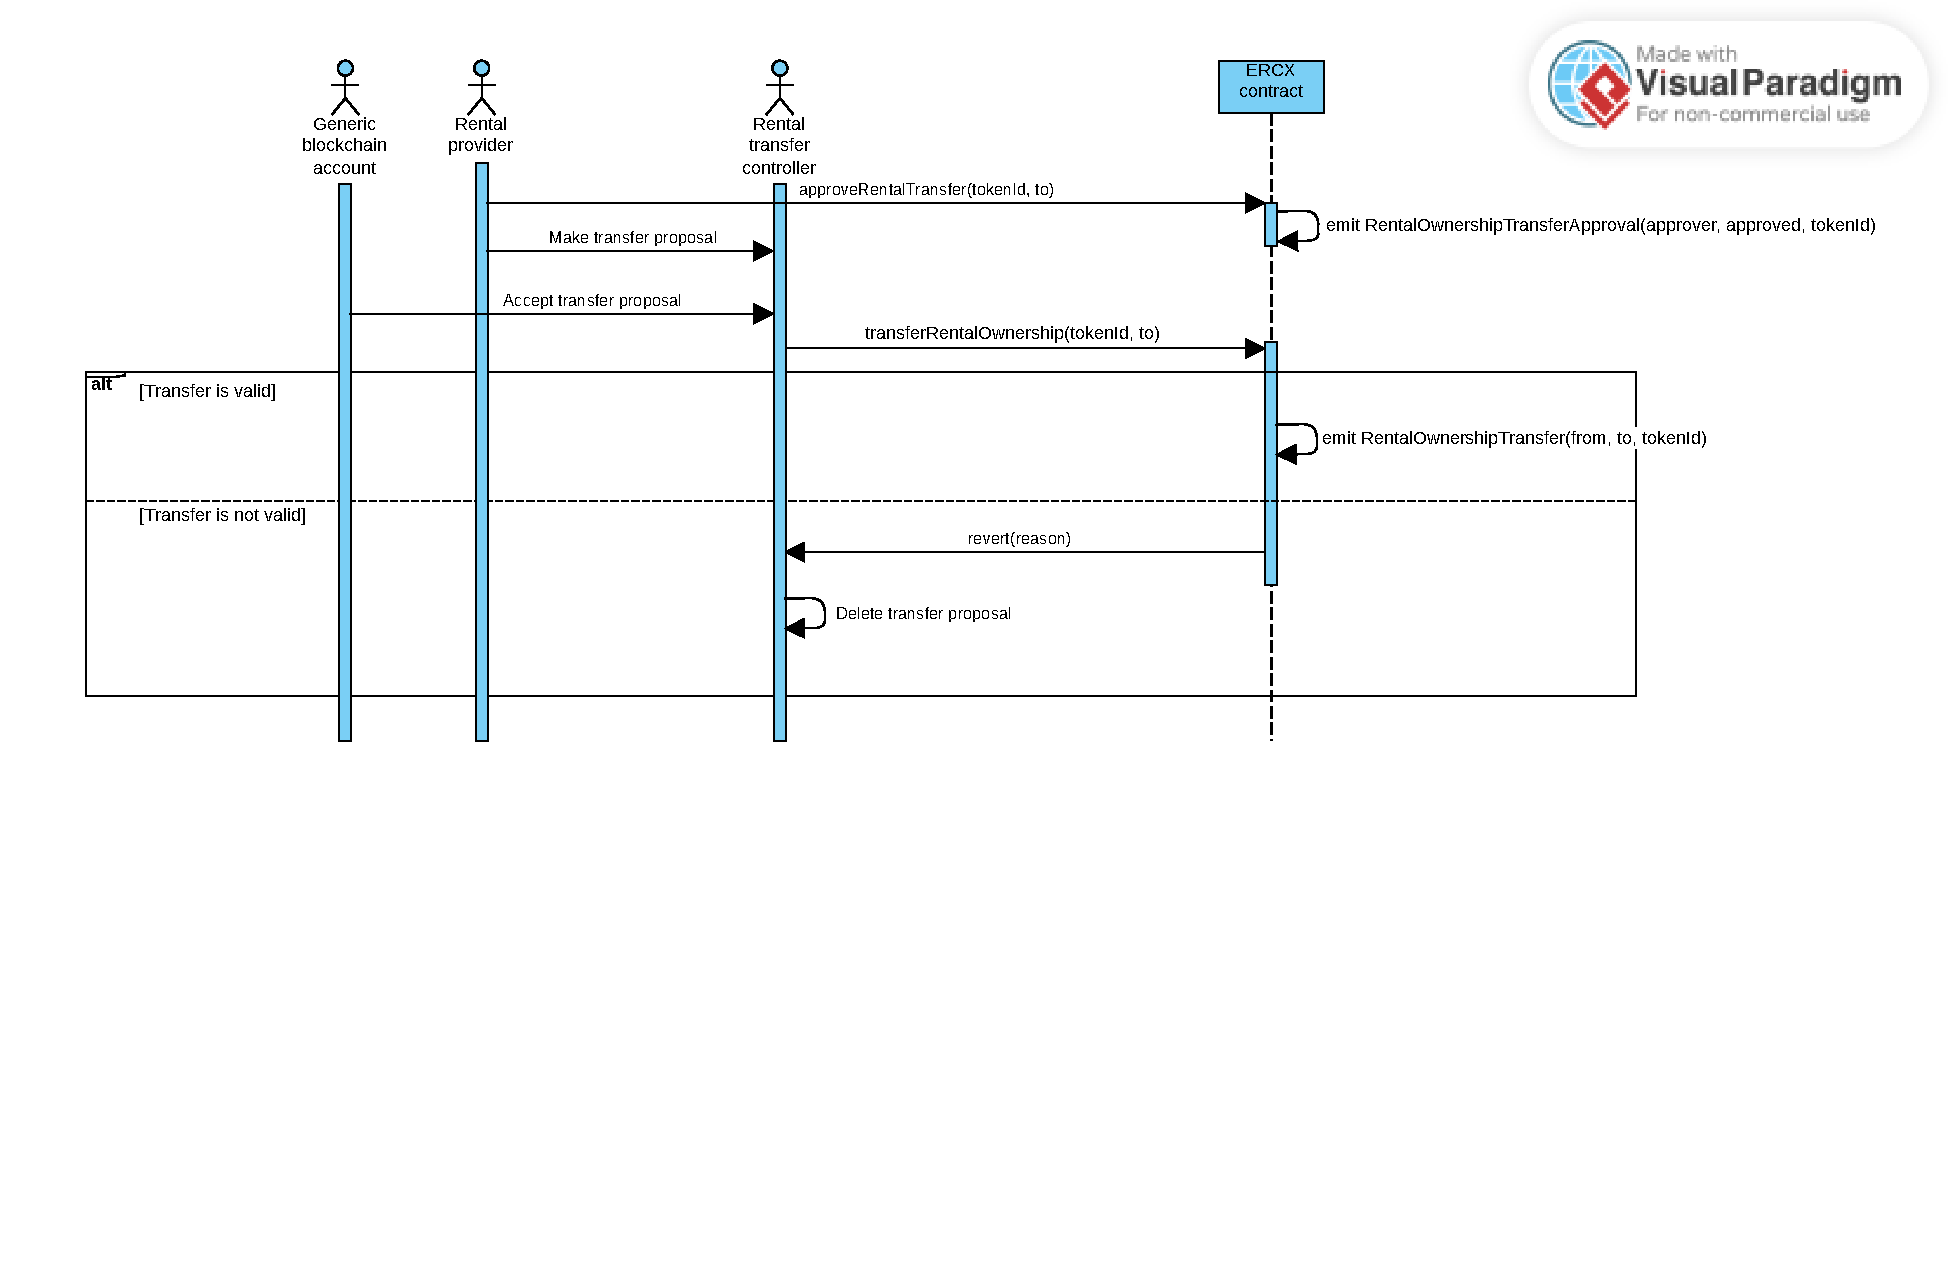
\includegraphics{SequenceDiagrams/sequence_rentalTransfer.pdf}}
        \end{adjustbox}
    \caption{Rental ownership transfer sequence diagram}
    \label{fig:RentalOwnerhipTransfer SD}
\end{figure}

As Fig.~\ref{fig:RentalOwnerhipTransfer SD} depicts, rental ownership transfer procedure is specular to the one seen for rented token transfer. Here, there is no need to call ERC721 \_transfer function, as the owner of the rented token does not need to be changed (only the rental provider is changed).\newline
\bigskip

\subsubsection{Rented token redemption}

\begin{figure}[H]
    \centering
        \begin{adjustbox}{width=1\textwidth}
            \fbox{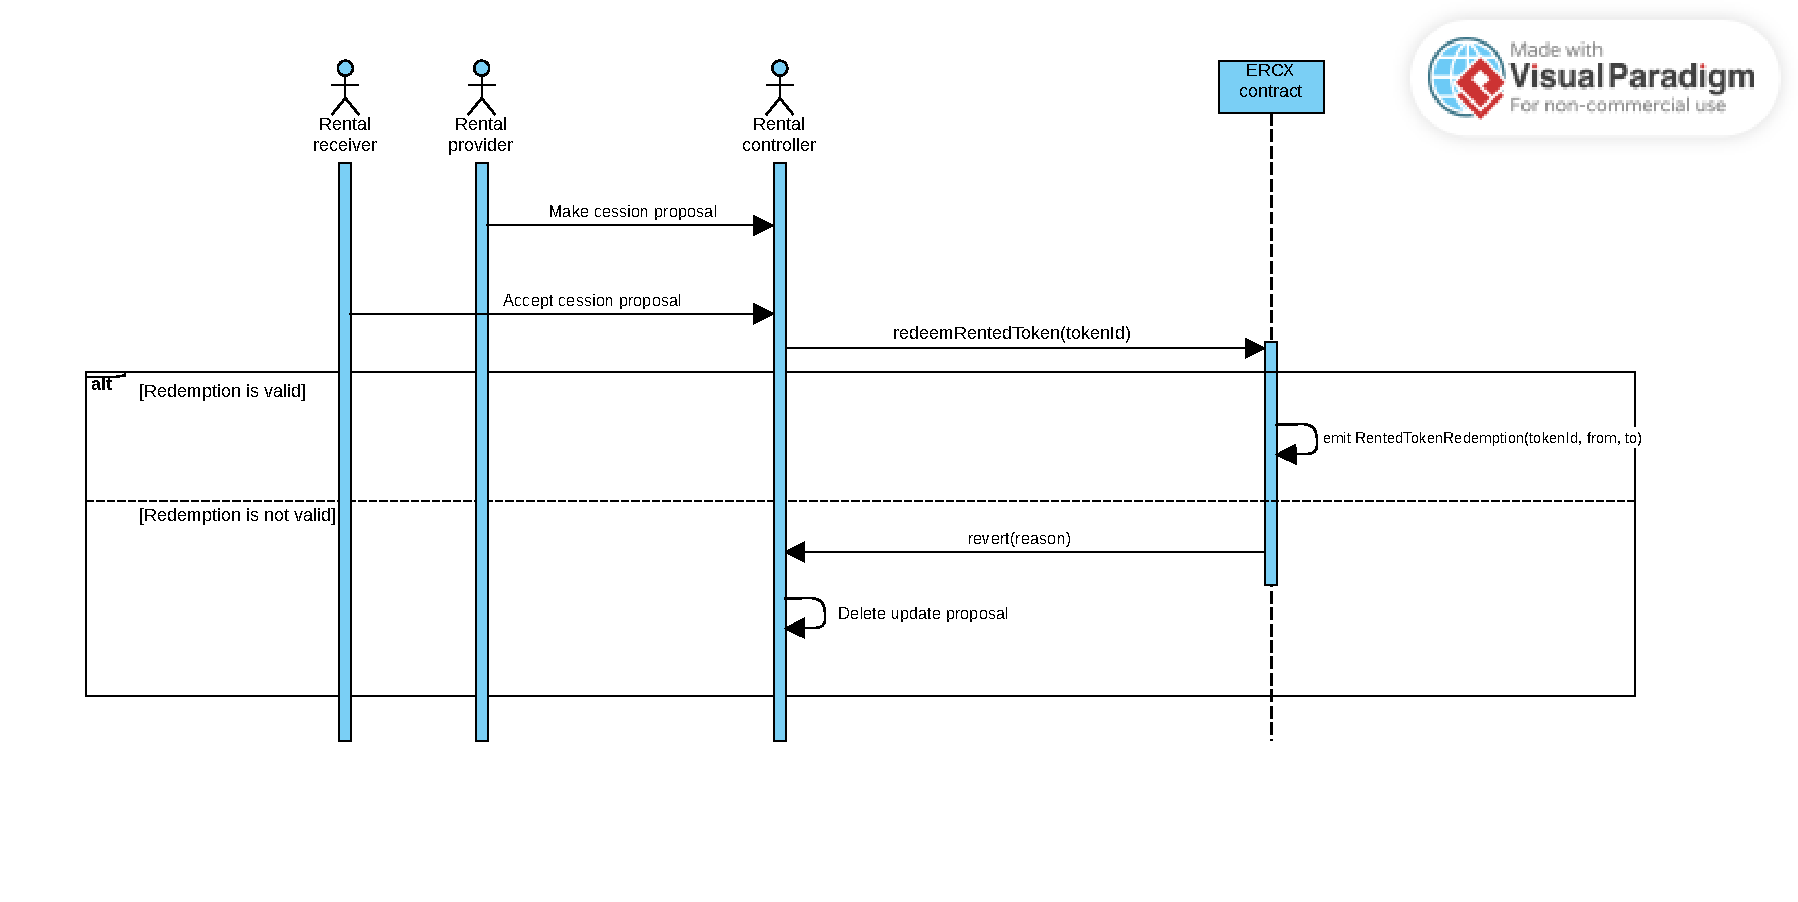
\includegraphics{SequenceDiagrams/sequence_rentedTokenRedemption.pdf}}
        \end{adjustbox}
    \caption{Rented token redemption sequence diagram}
    \label{fig:RentedTokenRedemption SD}
\end{figure}

Again, the process of redeeming a rented token, illustrated in Fig.~\ref{fig:RentedTokenRedemption SD}, is very similar to the ones discussed in the previous diagrams. Here we assumed that the rental is being controlled by a previously nominated intermediary, which will also be the one in charge to perform the token redemption using redeemRentedToken function, after the involved users find an agreement on the price.\newline
\bigskip

\subsubsection{Layaway}

\begin{figure}[H]
    \centering
        \begin{adjustbox}{width=1\textwidth}
            \fbox{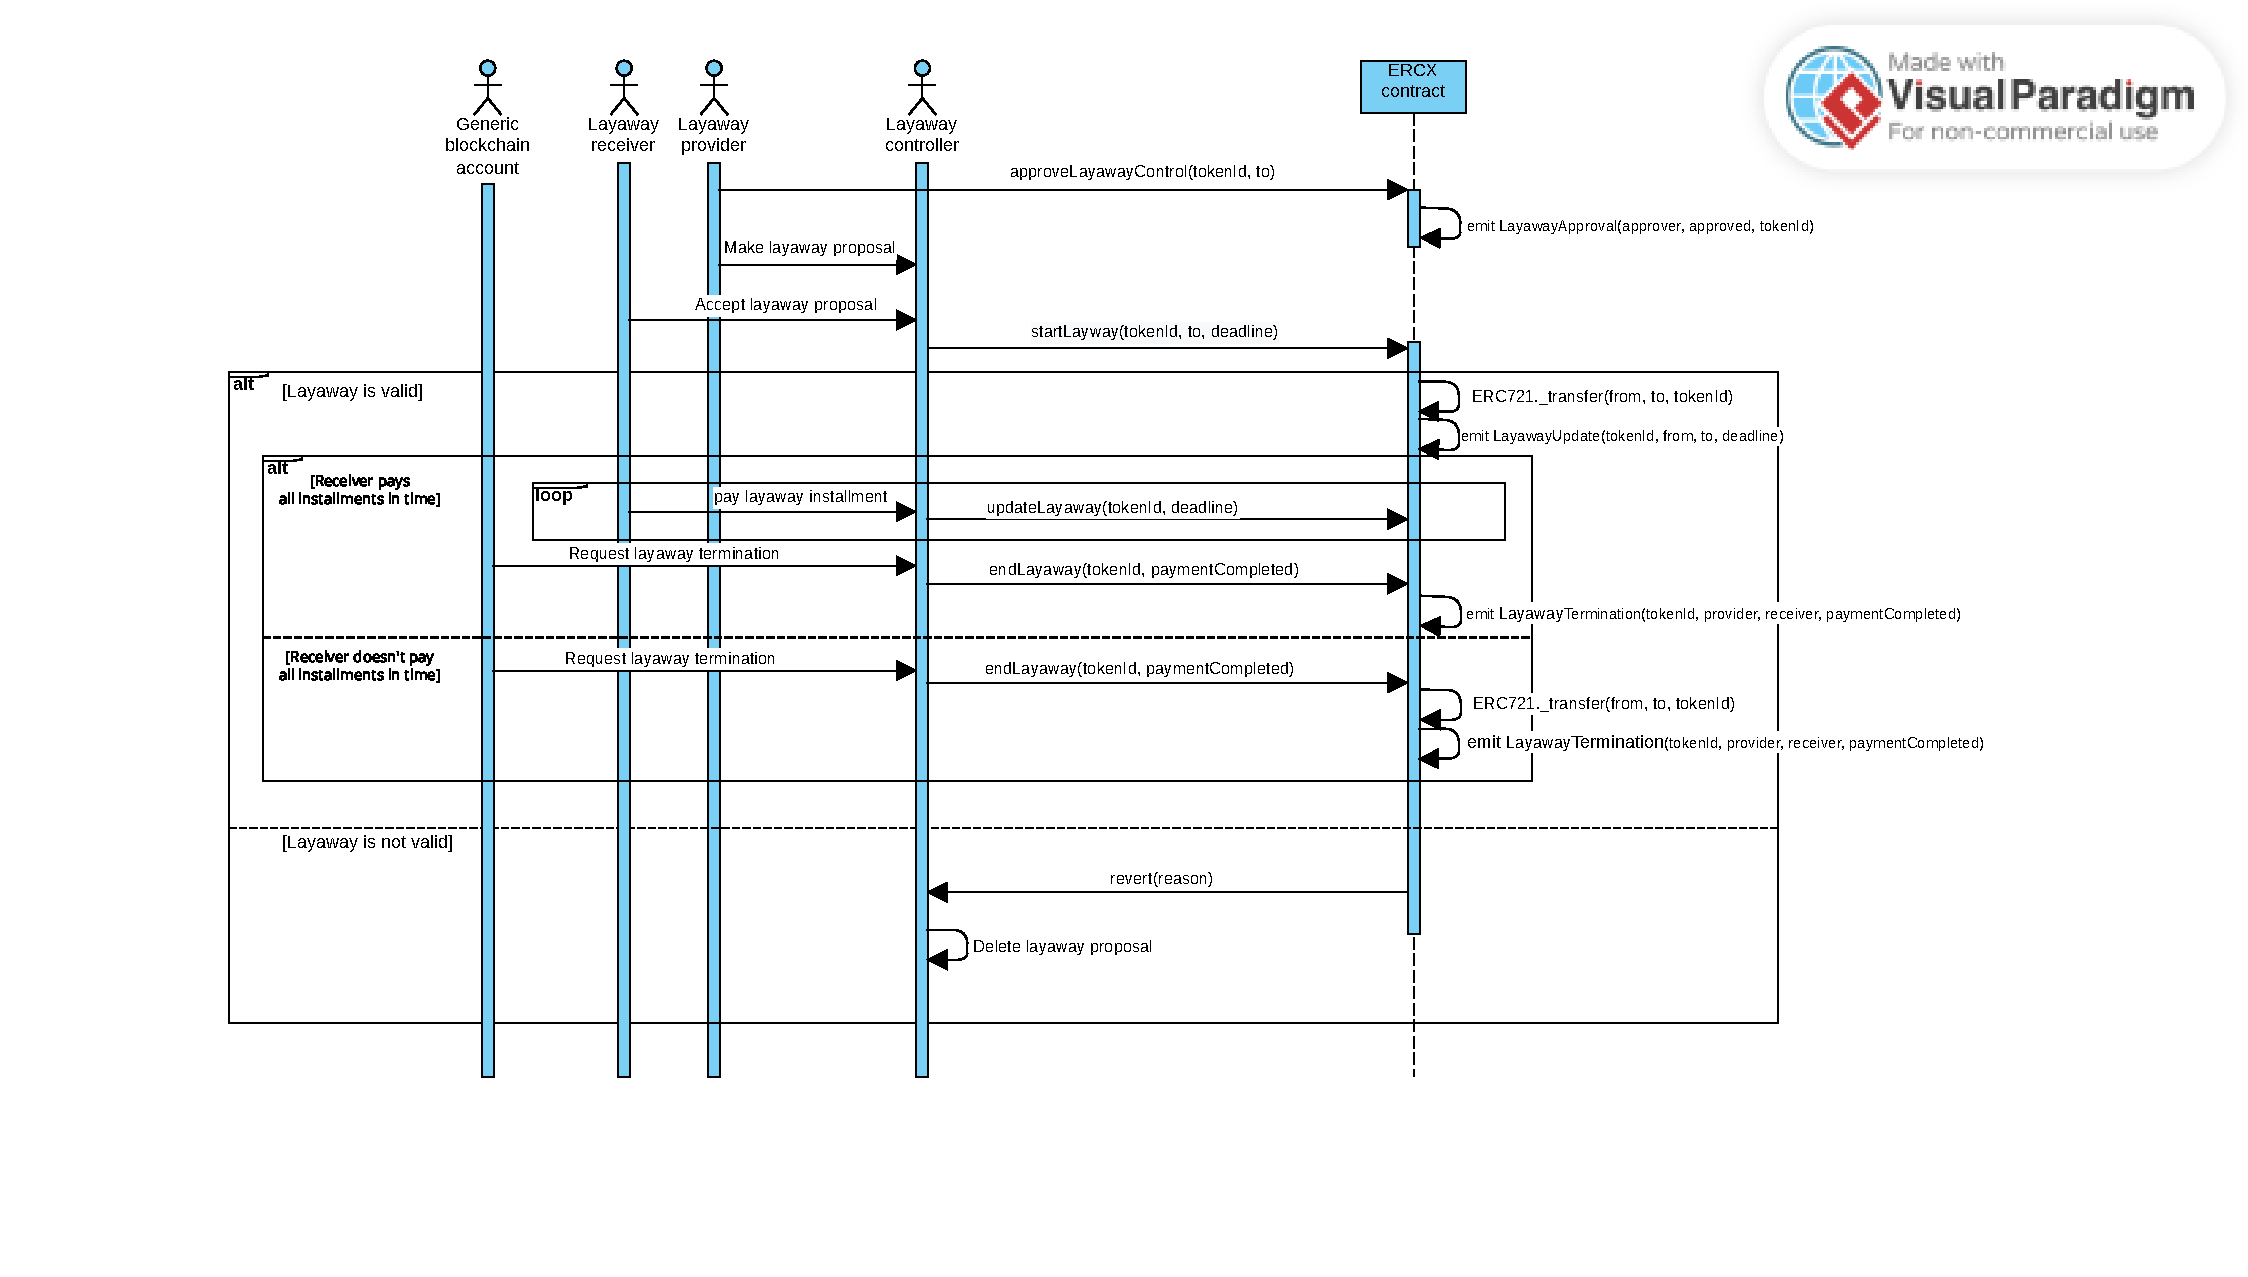
\includegraphics{SequenceDiagrams/sequence_layaway.pdf}}
        \end{adjustbox}
    \caption{Layaway sequence diagram}
    \label{fig:Layaway SD}
\end{figure}

Moving on to layaway diagram (Fig.~\ref{fig:Layaway SD}), we observe that the procedure used to start a layaway is the same used to start a rental, except for the fact that here the intermediary is mandatory. The event emitted on layaway start is named LayawayUpdate. For what concerns termination, instead, we see how the token can be kept by the layaway receiver if they pay all installments on time, or returned to the provider otherwise. In both cases, the function used for layaway termination is the endLayaway function, which can be called only by the layaway intermediary, which has the responsibility to state if the installment payments have been completed.\newline
When the receiver pays an installment, the intermediary will call updateLayawyay function, which will delay the deadline for the next installment payment and transfer the paid amount to the layaway provider.

\subsubsection{Transfers during layaway}

These last two diagrams, illustrated in Fig.~\ref{fig:LayawayedTokenTransfer SD} and Fig.~\ref{fig:LayawayOwnershipTransfer SD}, show the procedures used respectively for layawayed token transfer and layaway ownership transfer, which are completely analogous to the ones discussed for rental, hence don't need any further comments.

\begin{figure}[H]
    \centering
        \begin{adjustbox}{width=1\textwidth}
            \fbox{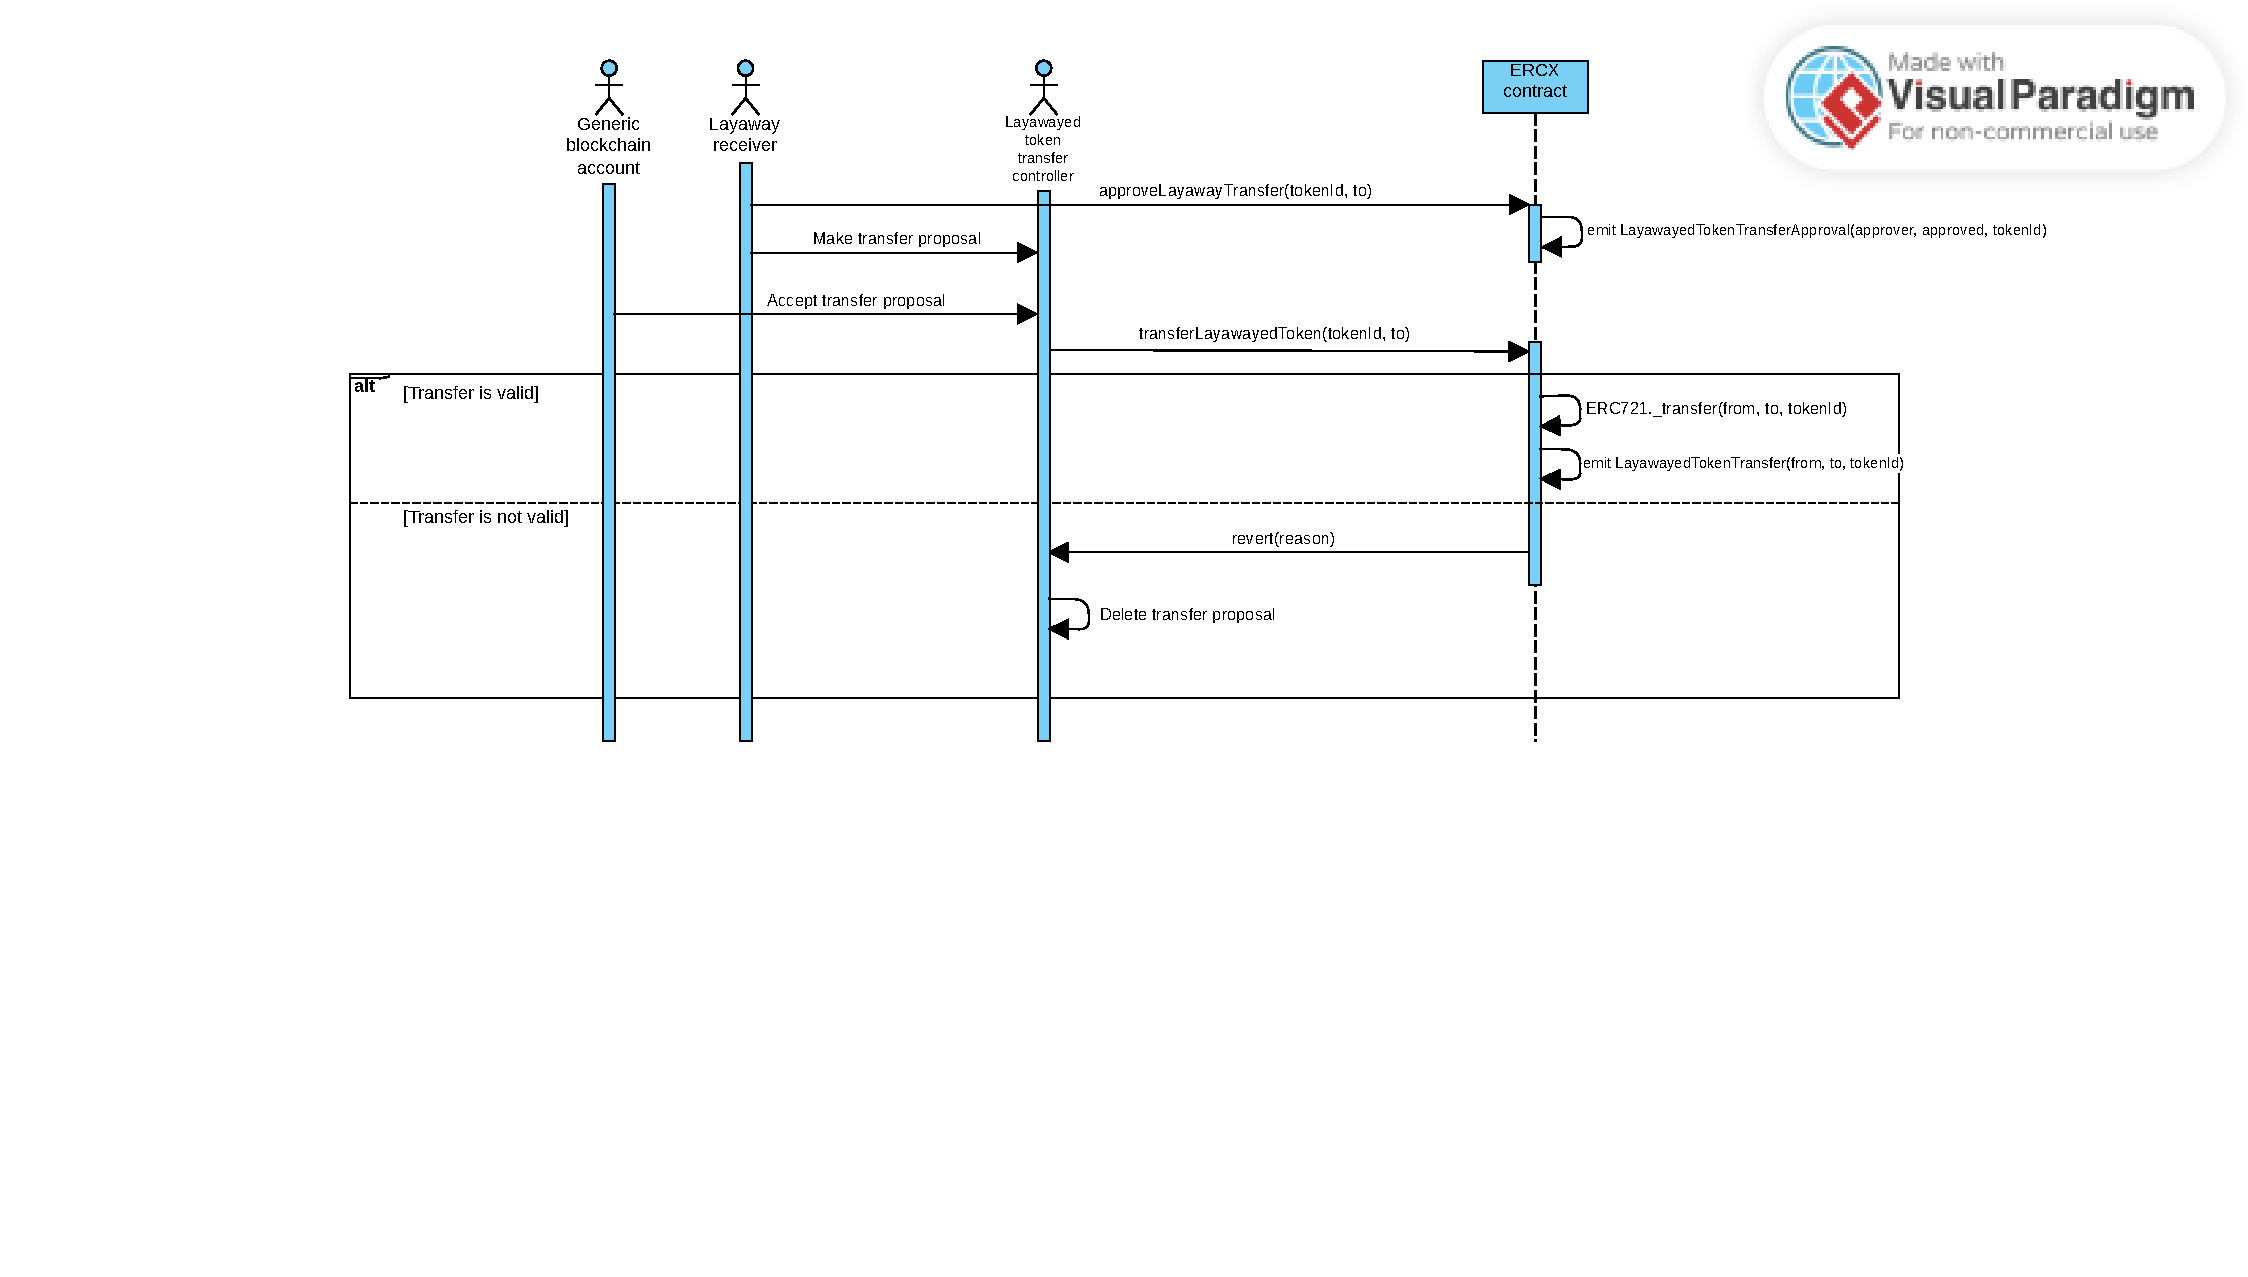
\includegraphics{SequenceDiagrams/sequence_layawayedTokenTransfer.pdf}}
        \end{adjustbox}
    \caption{Layawayed token transfer sequence diagram}
    \label{fig:LayawayedTokenTransfer SD}
\end{figure}

\begin{figure}[H]
    \centering
        \begin{adjustbox}{width=1\textwidth}
            \fbox{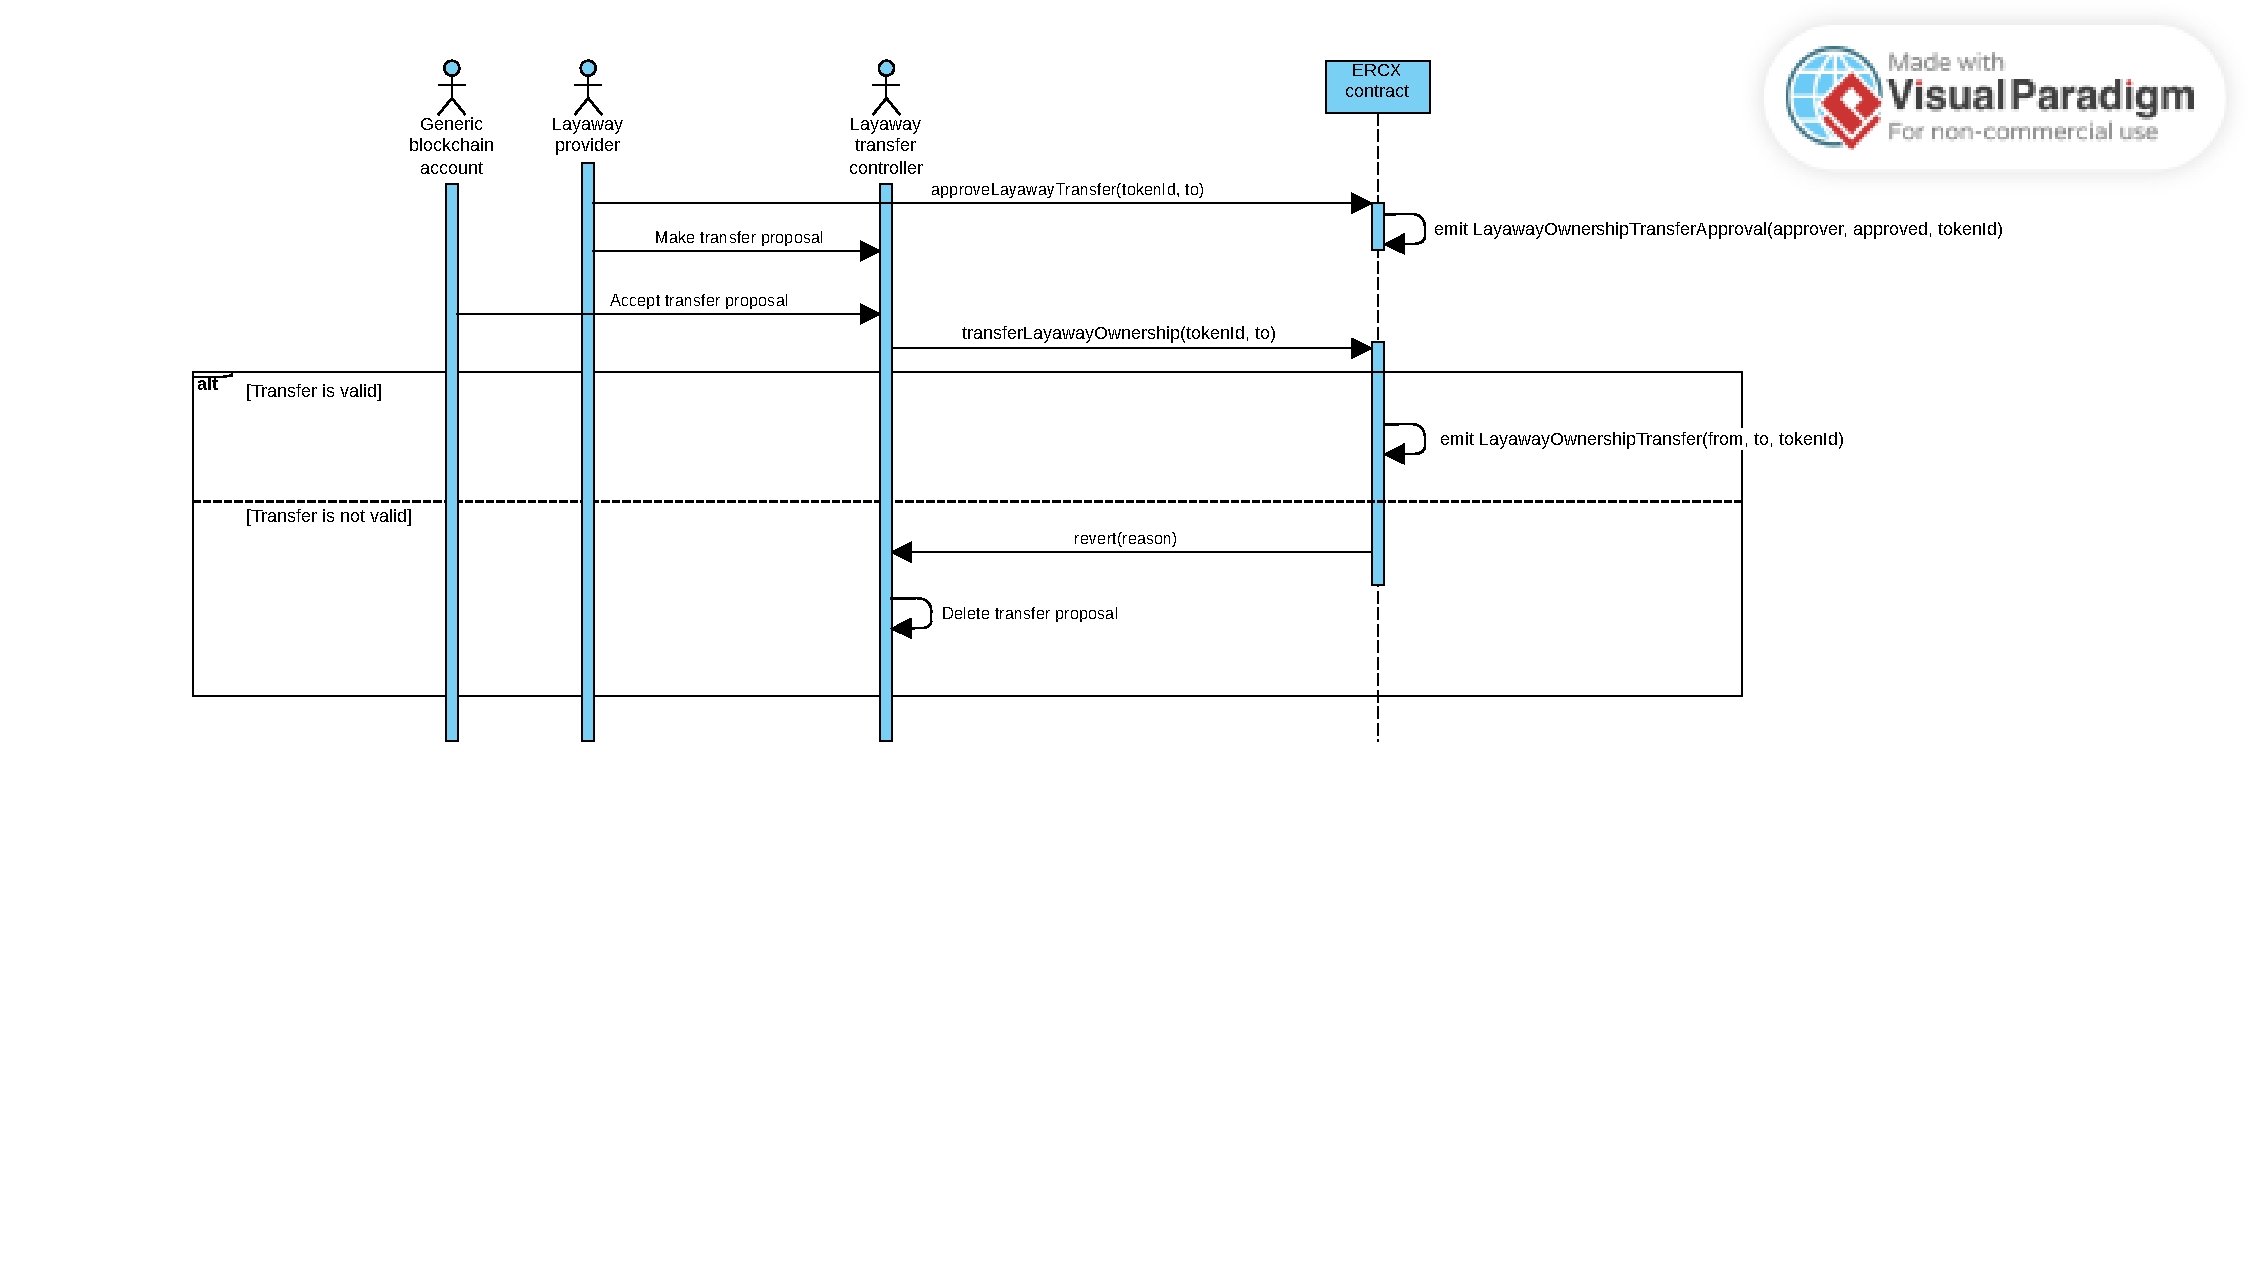
\includegraphics{SequenceDiagrams/sequence_layawayTransfer.pdf}}
        \end{adjustbox}
    \caption{Layaway ownership transfer sequence diagram}
    \label{fig:LayawayOwnershipTransfer SD}
\end{figure}

\section{Project repository}
The code and documentation of the proposed solution can be found at the following GitHub repository: \url{https://github.com/Andrea98Palermo/ERCX}. It contains the IERCX inteface,  ERCX token collection and intermediary contracts reference implementations, and also some unit tests performed on the solution. These tests will be described more accurately in the next chapter.

\bigskip
\bigskip
This concludes the presentation of the proposed solution; next chapter will pertain the solution's evaluation and the used testing methodologies.


\chapter{Solution evaluation}
\label{chap:3}
Having analyzed the structure and behaviour of the proposed solution, we can now move on to discuss about its evaluation.

\section{Tests}
The reference implementation has been tested using Hardhat\cite{ref:hardhat} testing environment. Hardhat is a development environment that facilitates building and debugging on Ethereum. It helps developers manage and automate the recurring tasks that are inherent to the process of building smart contracts and dApps. It also comes built-in with Hardhat Network, a local Ethereum network designed for development. \newline
In our case, Hardhat was used to compile the smart contracts, deploy them on the local simulated network, and perform unit tests on them. These unit tests are written in javascript, making use of some Hardhat specific libraries, and can be found in the tests folder in the project repository. \newline
The tests are designed to stress each functionality offered by the solution, and each of them comes with a string description which allows to understand exactly what its purposes are. Each functionality which can be carried out using an intermediary has been tested both with an EOA and a smart contract intermediary. The intermediary contracts used for this purpose are the reference rental and layaway marketplaces implementations, contained in the project repository.

\section{Complexity of the solution}
As the reader may have understood going trough the previous chapter, this solution is characterized by a significative complexity. This is the case mainly because of the decision of avoiding the creation of new user roles other than the owner defined in ERC721 standard, which entails the discussed advantages. This causes having to perform some additional operations and checks, in order to maintain consistency during the whole ERCX token lifecycle. \newline
Other than this, also the addition of subrental capabilities causes the complexity to grow: the details of a token's active rentals cannot be contained in a simple data structure, but have to be stored in an array; as expected, array usage increases complexity, not only because of the bigger and dynamic storage space used, but also for the operations that have to be performed on them. \newline
In this solution, the high complexity is particularly problematic for two reasons: first, being it composed of smart contracts, the complexity translates in gas fees that need to be paid in order to deploy and use the contracts. The gas costs of the solution have been studied and will be showcased in the next section. Moreover, being the solution meant to become a standard, its comprehensibility is extremely important. This potential issue has been addressed by documenting all the solution's components in the most accurate possible way, with all the diagrams discussed in the previous chapter.

\subsection{Gas costs analysis}
Whenever a smart contract is deployed to a blockchain or invoked, several operations need to be performed on every single node of the blockchain. For smart contract function calls, this means executing the function code and modifying the contract's state on every node; for contract deployment, instead, each node will have to store the contract code (which is contained inside the deployment transaction). In order to avoid network clogging and denial of service attacks, blockchain protocols require the account which performs these operations to pay a so called gas fee, which is proportional to the complexity of the requested operation. This means that the more a function is complex, the more its invocation will cost; similarly, the longer a smart contract's code is, the more its deployment will cost.\newline
Gas fees are paid in the blockchain's native cryptocurrency, and on EVM-compatible chains they are calculated in terms of gas units: each low level operation has an associated cost in gas units; the cost of calling a function is given by the sum of the costs of all the low level operations that the function performs. To convert the gas cost in the corresponding actual cryptocurrency amount, the obtained number of gas units must be multiplied by the price of a single gas unit; in Ethereum, the price of a unit is given by the sum of a base fee and a priority fee. The base fee is calculated by the protocol in function of the network utilization, while the priority fee is set by the function caller as an incentive for the validators to process their transaction before the other ones.\newline
Here we report an approximation of the price of the ERCX reference implementation contract deployment and each of its functions in terms of gas units. Note that the functions' prices are not fixed, as when the contract's data structures grow, the functions interacting with them could become more complex. These results were obtained using hardhat-gas-reporter npm pacakge, which can be found at \url{https://www.npmjs.com/package/hardhat-gas-reporter}. Some functions have been omitted, as they are declared as \textit{view}: this means that they do not modify the contract's state and only read from it. View functions will not cost gas if called from outside the blockchain, as the function can be resolved in the local node that is being used to connect to the network without submitting a transaction.
On the other hand, if a view function in a contract is called from another contract, it will cost gas, as the read from the state has to be performed on every node. \newline
Table~\ref{tab:Gas report} was obtained using the gas reporter tool, and shows for each function the maximum, minimum and average gas cost observed when running the tests.\newline
The ERCX contract deployment costed 4149775 gas units, while LayawayMarketplace and RentalMarketplace deployments costed respectively 1654300 and 3351093 gas units. This cost is, as expected, much higher than the functions' cost.

\begin{table}
\centering
\begin{adjustbox}{width=0.75\textwidth}
\small
\begin{tabular}{@{}cccccc@{}}
\toprule
\textbf{Contract}  & \textbf{Function}            & \textbf{Min} & \textbf{Max} & \textbf{Avg} & \textbf{\#calls} \\ \midrule
ERCX               & approve                      & 53406        & 53406        & 53406        & 1                \\
ERCX               & approveLayawayControl        & 53571        & 53583        & 53583        & 24               \\
ERCX               & approveLayawayTransfer       & 48857        & 51108        & 50143        & 7                \\
ERCX               & approveRentalControl         & 50970        & 50982        & 50982        & 37               \\
ERCX               & approveRentalTransfer        & 37209        & 54059        & 45634        & 6                \\
ERCX               & endLayaway                   & 37564        & 71263        & 52131        & 7                \\
ERCX               & endRental                    & 63332        & 94496        & 74723        & 23               \\
ERCX               & redeemRentedToken            & 45758        & 48220        & 46989        & 2                \\
ERCX               & startLayaway                 & 98242        & 98254        & 98253        & 18               \\
ERCX               & startRental                  & 146030       & 178294       & 165228       & 37               \\
ERCX               & startSubrental               & 127785       & 149697       & 146773       & 30               \\
ERCX               & transferLayawayedToken       & 75418        & 75418        & 75418        & 3                \\
ERCX               & transferLayawayOwnership     & 36628        & 38572        & 37276        & 3                \\
ERCX               & transferRentalOwnership      & 65068        & 84824        & 73342        & 5                \\
ERCX               & transferRentedToken          & 69872        & 77616        & 72970        & 5                \\
ERCX               & updateLayaway                & 36311        & 36311        & 36311        & 2                \\
ERCX               & updateRental                 & 39334        & 44157        & 41134        & 4                \\
LayawayMarketplace & acceptLayawayProposal        & 301298       & 301298       & 301298       & 3                \\
LayawayMarketplace & acceptTransferProposal       & 84812        & 123717       & 104265       & 4                \\
LayawayMarketplace & endLayaway                   & 89760        & 120825       & 100115       & 3                \\
LayawayMarketplace & makeLayawayProposal          & 200884       & 200884       & 200884       & 3                \\
LayawayMarketplace & makeLayawayTransferProposal  & 148677       & 151739       & 150208       & 2                \\
LayawayMarketplace & payLayawayInstallment        & 55429        & 55429        & 55429        & 2                \\
RentalMarketplace  & acceptRedemptionProposal     & 103640       & 103640       & 103640       & 2                \\
RentalMarketplace  & acceptRentalProposal         & 213877       & 213877       & 213877       & 6                \\
RentalMarketplace  & acceptSubrentalProposal      & 203109       & 203109       & 203109       & 1                \\
RentalMarketplace  & acceptTransferProposal       & 133214       & 134690       & 133952       & 4                \\
RentalMarketplace  & acceptUpdateProposal         & 95831        & 95831        & 95831        & 2                \\
RentalMarketplace  & makeRentalProposal           & 202676       & 202676       & 202676       & 6                \\
RentalMarketplace  & makeRentalRedemptionProposal & 157664       & 157664       & 157664       & 1                \\
RentalMarketplace  & makeRentalTransferProposal   & 159075       & 160414       & 159745       & 2                \\
RentalMarketplace  & makeRentalUpdateProposal     & 174036       & 174036       & 174036       & 1                \\
RentalMarketplace  & makeSubrentalProposal        & 183552       & 183552       & 183552       & 1                \\ \bottomrule
\end{tabular}
\end{adjustbox}
\caption{Gas costs report}
\label{tab:Gas report}
\end{table}



\chapter{Conclusions}
As we stated, rental and layaway services would revolutionize the NFT ecosystem, allowing users to be able to use NFTs without actually buying them, and at the same time making NFTs a more liquid type of assets. \newline
Currently there exist some tentatives to implement these services, but each of them suffers the discussed fundamental limitations. Here, a different type of solution was proposed, which is aimed to overcome the disadvantages of the existing approaches. The proposed solution, on the other hand, as well suffers some different limitations, mainly caused by its significative complexity. Anyways, the gas costs have been analyzed and they are not unbearable: at the time of writing, the deployment of the ERCX contract on the Ethereum blockchain would cost around 140\$, while the functions would have costs in the 1.50\$-4.50\$ range. This calculation has been performed using a base fee of 21 gwei and a priority fee of 1 gwei: these values were taken from \url{https://etherscan.io/gastracker}, which shows the advised values of base and priority fees to be used in order to have a transaction processed in an acceptable amount of time. For what concerns other EVM-compatible chains, the calculation can be made in the same way, and the USD price is expected to be lower than the one seen for Ethereum, as gas fees as generally lower on these other chains.\newline
Another potential limitation caused by the solution's complexity is the lack of comprehensibility and usability, but these issues have been addressed trying to provide the most complete and understandable possible documentation. 

 \section{Future work}
 A possible field for future work could be the formalization and automation of the procedure needed to upgrade deployed ERC721 collections contracts to conform with ERCX standard. This would completely solve retro-compatibility issues, and allow any existing NFT to be rented or given on layaway without any effort. \newline
 Smart contracts are inherently immutable, but some workarounds have been found to be able to make modifications to a contract after its deployment: upgrading of smart contracts is an important and open research field, and there exist some works that aim to analyze the existing approaches and provide new ones. In \cite{ref:SCupgrade1}, after showcasing the existing solutions, the authors propose a novel approach, particularly focused on security against known smart contract attacks. In \cite{ref:SCupgrade2}, instead, the authors once again discuss the existing methodologies, and also propose a completely automated solution that is able to make modifications to smart contracts. Currently, as far as the author knows, the most used upgradability solution is the one designed by Openzeppelin, which can be found at \url{https://docs.openzeppelin.com/learn/upgrading-smart-contracts}. This approach relies on a proxy contract, which has a reference to the address of the real implementation contract. This address can be later changed by some authorized accounts, allowing to deploy an upgraded implementation contract, which will be accessed through the proxy contract, that never changes.\newline
 The automation of such procedure would make the integration of rental and layaway capabilities much easier for the already deployed ERC721 tokens collections, making the proposed solution fully retro-compatible.

\backmatter
\phantomsection
\begin{thebibliography}{17}

\bibitem{ref:nfts}
W. Rehman, H. e. Zainab, J. Imran and N. Z. Bawany, \textit{"NFTs: Applications and Challenges"}, 2021 22nd International Arab Conference on Information Technology (ACIT), Muscat, Oman, 2021, pp. 1-7, \url{https://doi.org/10.1109/ACIT53391.2021.9677260}.

\bibitem{ref:NFT applications}
Despotovic, V., Bjelica, D., and Barać, D. (2022). \textit{"Analysis of potential NFT applications"}. E-Business Technologies Conference Proceedings, 2(1), 103–107. Retrieved from \url{https://ebt.rs/journals/index.php/conf-proc/article/view/136}.

\bibitem{ref:liquidation}
Kaihua Qin, Liyi Zhou, Pablo Gamito, Philipp Jovanovic, and Arthur Gervais. 2021. \textit{"An empirical study of DeFi liquidations: incentives, risks, and instabilities"}. In Proceedings of the 21st ACM Internet Measurement Conference (IMC '21). Association for Computing Machinery, New York, NY, USA, 336–350. \url{https://doi.org/10.1145/3487552.3487811}.

\bibitem{ref:EIP4907}
Anders (@0xanders), Lance (@LanceSnow), Shrug <shrug@emojidao.org>, \textit{"ERC-4907: Rental NFT, an Extension of EIP-721,"} Ethereum Improvement Proposals, no. 4907, March 2022. [Online serial]. Available: \url{https://eips.ethereum.org/EIPS/eip-4907}.

\bibitem{ref:EIP721}
William Entriken (@fulldecent), Dieter Shirley <dete@axiomzen.co>, Jacob Evans <jacob@dekz.net>, Nastassia Sachs <nastassia.sachs@protonmail.com>, \textit{"ERC-721: Non-Fungible Token Standard"}, Ethereum Improvement Proposals, no. 721, January 2018. [Online serial]. Available: \url{https://eips.ethereum.org/EIPS/eip-721}.

\bibitem{ref:EVM}
Ethereum Virtual Machine documentation, \url{https://ethereum.org/en/developers/docs/evm/}.

\bibitem{ref:renft}
ReNFT, \url{https://docs.renft.io}.

\bibitem{ref:vera}
Vera Financial, \url{https://docs.vera.financial/hub/}.

\bibitem{ref:double}
Double protocol, \url{https://docs.double.one}.

\bibitem{ref:supermojo}
Supermojo, \url{https://supermojo.com}.

\bibitem{ref:teller}
Teller Finance, \url{https://teller.gitbook.io/teller-v2}.

\bibitem{ref:openzeppelin}
Openzeppelin, \url{https://www.openzeppelin.com}.

\bibitem{ref:hardhat}
Hardhat, \url{https://hardhat.org/docs}.

\bibitem{ref:SCupgrade1}
V. C. Bui, S. Wen, J. Yu, X. Xia, M. S. Haghighi and Y. Xiang, \textit{"Evaluating Upgradable Smart Contract,"} 2021 IEEE International Conference on Blockchain (Blockchain), Melbourne, Australia, 2021, pp. 252-256, doi: 10.1109/Blockchain53845.2021.00041.

\bibitem{ref:SCupgrade2}
Rodler, Michael, Wenting Li, Ghassan O. Karame and Lucas Davi. \textit{“EVMPatch: Timely and Automated Patching of Ethereum Smart Contracts.”} USENIX Security Symposium (2020).



\end{thebibliography}

\end{document}